\documentclass[12pt]{book}
\usepackage[portuguese]{babel}
\usepackage{indentfirst}
\usepackage{graphicx}
\usepackage{caption}
\usepackage{verse}
\usepackage{subcaption}
\usepackage{multirow}
\usepackage{array}
\newcolumntype{M}[1]{>{\centering\arraybackslash}m{#1}}
\def\CC#1{\makebox[4in]{#1}}

\title{Notas de aula}

\begin{document}
	
	\setcounter{chapter}{-1}
	
	\maketitle
	
	\frontmatter
	\chapter{Notas}
	\par Assuntos pendentes/incompletos:
	\begin{enumerate}
		\item Anteriores ao Humanismo. Conferir com o Eduardo e o Guglielmo.
		\item \textit{A divina comédia}. Procurar anotações nos cadernos.
		\item \textit{Os sermões}. Procurar anotações no OneDrive.
		\item \textit{Auto da barca do inferno}. Procurar anotações no OneDrive.
		\item As vertentes dos sonetos de Camões. Procurar anotações nos cadernos (a parte sobre Maneirismo estava no caderno de Geografia).
		\item A arte barroca no Brasil. Procurar anotações nos cadernos.
		\item \textit{Cartas chilenas}. (?)
		\item \textit{O Uruguai}. (?)
		\item \textit{Frankenstein}. Procurar anotações no OneDrive.
	\end{enumerate}
	
	\listoffigures
	\tableofcontents
	
	\mainmatter
	\chapter{\O}
	Espaço destinado para futuros acréscimos.
	
	\part{Humanismo}
	
		\chapter{Introdução}
		\par O termo \textbf{estilo} tem origem no latim \textit{stilus}, instrumento metálico utilizado para escrever ou desenhar. Com o tempo, passou a designar, no campo artístico, a forma pela qual determinada expressão ou modo particulariza-se, marcava a sociedade. De maneira geral, o estilo pode ser \textbf{autoral} - exprime características que descrevem o texto de um determinado autor -, ou de \textbf{época} - presença de características compartilhadas por autores de um mesmo período. Como convenção, utilizarei iniciais maiúsculas para me referir aos estilos de época, como forma de evitar confusões ao longo da leitura. Tal processo ficará mais claro na parte do Realismo, e a distinção feita com o realismo presente em algumas obras do Romantismo brasileiro.
		\par O Humanismo situa-se na passagem da Idade Média para a Idade Moderna e, em especial, na relação\footnote{Uma analogia curiosa utilizada para descrever tal processo é a figura de um indivíduo, apoiado sobre o termo ``centrismo'', com os pés divididos entre ``teo/antropo''.} entre o \textbf{teocentrismo} e o \textbf{antropocentrismo}. Entre os principais autores desse período, destacam-se os italianos Dante Alighieri (1265-1321), autor de \textit{A divina comédia}, e Francesco Petrarca (1304-1374), autor de \textit{Cancioneiro}.
		\par Na figura que se segue, é representado um dos desenhos realizados em sala de aula, ao longo da abordagem da visão de mundo do indivíduo humanista. O recurso utilizado é chamado de \textbf{alegoria}, uma metáfora prolongada que serve de representação concreta para alguma ideia ou conceito abstrato.
		\par \textbf{Carece de mais informações.}
		\begin{figure}[h]
			\centering
			\includegraphics[width=4cm]{figura_1}
			\caption{Legenda aqui.}
			\label{fig:mesh1}
		\end{figure}
	
		\chapter{Humanismo em Portugal}
		\par O marco inicial do Humanismo em Portugal são as crônicas de Fernão Lopes (1380-1460). Vale lembrar que a \textbf{crônica}, na concepção da Idade Média, é uma forma de gênero historiográfico que expressava uma visão \textbf{providencial}\footnote{Providência divina como a vontade de Deus manifesta. Mais adiante, na epopeia classicista \textit{Os lusíadas}, veremos novamente a providência, descrita no último canto, pela forma como Deus conduz a realidade.} da história, na qual Deus interfere no destino humano com o intuito de ensinar (caráter exemplar). É interessante notar que Fernão Lopes introduzira na historiografia ocidental a noção da História como resultado das ações, vontades humanas, em um contexto específico.
		\par \textbf{Carece de mais informações.}
		
	\part{Classicismo}
	
		\chapter{Introdução}
 		\par A gênese do Classicismo remonta ao início da Idade Moderna, em meio ao processo de transição do \textbf{feudalismo} para o \textbf{capitalismo mercantil} (primeira fase). O \textbf{Renascimento} é o marco inicial do Classicismo, compreendendo a retomada dos valores estéticos e culturais da Antiguidade Clássica (greco-romana).
 		\par Entre os valores, destacam-se:
 		\begin{itemize}
 			\item Harmonia.
 			\item Equilíbrio
 			\item Proporção e simetria (verismo anatômico).
 			\item Racionalidade.
 			\item Antropocentrismo.
 			\item Hedonismo (contemplação estética, o corpo humano como belo).
 		\end{itemize}
 		\par A pintura \textit{Primavera} (Figura 3.1), do italiano Sandro Botticelli (1445-1510), sintetiza importantes valores do período. Analisá-la-emos em momento oportuno, ao tratarmos do Arcadismo no Brasil. 
 		\begin{figure}[h]
 			\centering
 			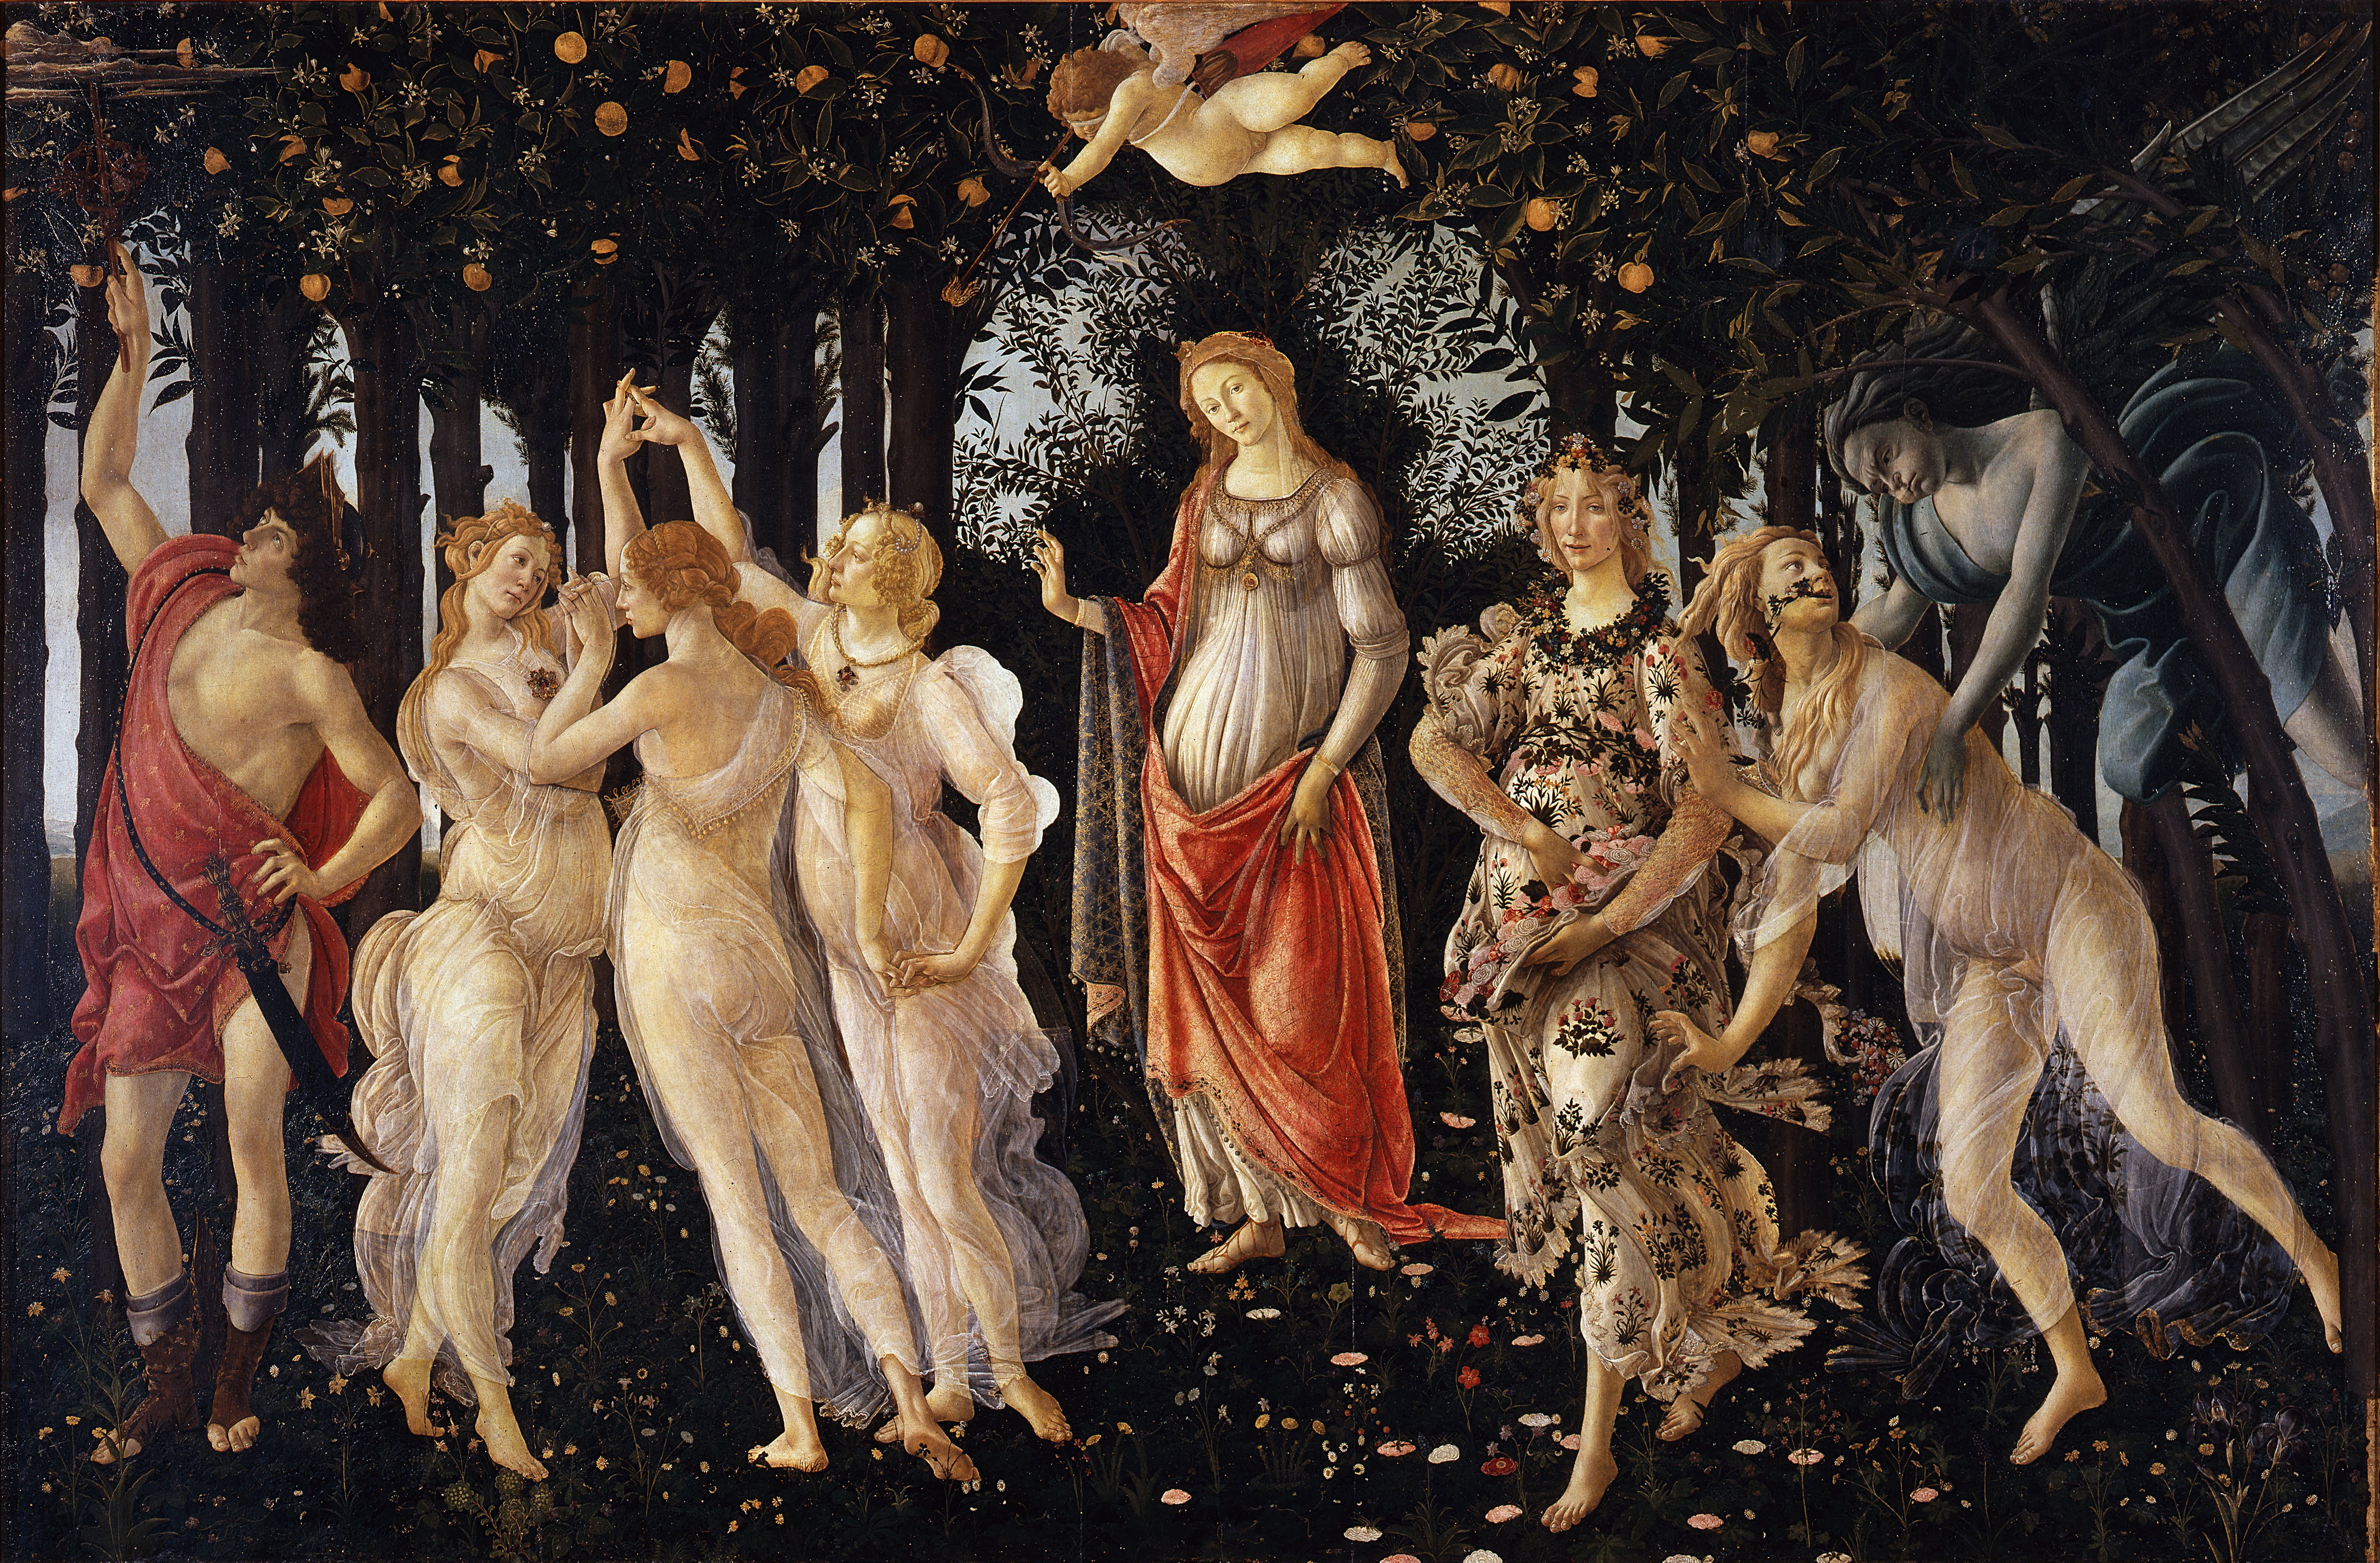
\includegraphics[width=4cm]{figura_2}
 			\caption{Legenda aqui.}
 			\label{fig:mesh2}
 		\end{figure}
 		\par Também é válido mencionar, como curiosidade, a técnica de escorço utilizada na escultura \textit{Davi} (Figura 3.2), de Michelangelo (1475-1564), como forma de produzir profundidade, extensão na visão do espectador corretamente posicionado (é extremamente difícil, se não impossível, encontrar alguma fotografia que registre decentemente tal perspectiva).
 		\begin{figure}[h]
 			\centering
 			\includegraphics[width=4cm]{figura_3}
 			\caption{Legenda aqui.}
 			\label{fig:mesh3}
 		\end{figure}

 		\chapter{A literatura classicista}
 		\par \textbf{Clássico} é a obra que supera a barreira do tempo, mantendo o interesse das gerações posteriores e servindo de modelo dos valores universais. Uma das características mais presentes nesse estilo é a \textbf{emulação} (imitação, competição) de tais clássicos (exemplo de \textbf{lugar-comum}, tema que se repete na tradição literária). Note, nesse sentido, que não necessariamente se buscava originalidade.
 		
 		\chapter{Classicismo em Portugal}
 		\par Sá de Miranda (1481-1558) fora o introdutor do Classicismo em Portugal. Utilizara o chamado \textbf{doce estilo novo} (de origem na poesia lírica humanista desenvolvida na Itália), o qual inaugurava uma nova medida - o verso decassílabo, com dez sílabas poéticas. Em relação a esse novo estilo, cabe lembrar:
 		\begin{itemize}
 			\item Métrica é a medida para o número de sílabas poéticas de um verso.
 			\item Escansão é o processo de contagem das sílabas poéticas de um verso.
 			\item Icto é a tônica obrigatória. Para o caso de um verso decassílabo, ictos na quarta e oitava silabas poéticas formam um verso decassílabo sáfico, ao passo que um icto na sexta forma um verso decassílabo heroico.
 			\item Versos em redondilha menor e maior possuem, respectivamente, cinco e sete sílabas poéticas.
 			\item Por fim, como curiosidade, versos com onze sílabas poéticas são chamados de hendecassílabos.
 		\end{itemize}
 	
 		\chapter{Luís de Camões}
 		\par \textbf{Carece de mais informações.}
 			\section{Sonetos}
 			\par Novamente, há o processo de emulação dos clássicos da Antiguidade, por meio de sonetos de e sobre amor que, de maneira geral, buscam o definir, e não o expressar. Nota-se a sublimação da figura feminina, assim como uma concepção platônica de amor perfeito entre as almas (e paixão entre corpos). Relembre, em relação ao amor platônico, o episódio grego da \textbf{gigantomaquia}.
 			\par Lembre-se da distinção entre o plano das ideias e o plano sensível. Há uma abordagem analítica e universalista do amor, uma reflexão racional sobre a natureza do sentimento amoroso (o que é o amor?). O eu lírico encarna a natureza humana (concepção universal, que não aborda um amor particular, mas do amor que seria sentido por qualquer pessoa).
 				\subsection{Vertentes dos sonetos de Camões}
 				\par \textbf{Carece de mais informações.}
 			\section{Os lusíadas}
 			\par Trata-se de uma \textbf{epopeia}, poema épico\footnote{O gênero épico se baseia na narração dos feitos de um herói, por meio de uma linguagem grandiloquente e tom heroico.} de longa extensão. O herói em questão é Vasco da Gama (1469-1524), navegador português responsável por estabelecer uma rota comercial marítima entre a Europa e as Índias. Com efeito, a obra fora escrita no contexto das \textbf{Grandes Navegações}. 
 			\par A obra é escrita em versos decassílabos heroicos, i.e., com dez sílabas poéticas e icto na sexta. Possui um esquema de rimas em oitava - sistema ABABACC, e é dividida em um total de dez cantos. A emulação dos clássicos, assim como nos sonetos, também se faz presente. Em especial, emula a \textit{Eneida}, de Virgílio (70 a.C.-19 d.C.). Note, novamente, que a originalidade não era algo fundamental para os autores da época.
 			\par A obra é dividia em três partes:
				\subsection{Introito} 			
 				\begin{enumerate}
 					\item \textbf{Proposição}: o poeta apresenta o assunto do poema. Nessa parte inicial, é interessante notar a forma pela qual as armas, em processo de metonímia, referem-se aos indivíduos que as utilizam. Os guerreiros e barões são abordados como nobres, que se destacam ao partirem das praias de Portugal em direção às Índias (``além da taprobana''), viagem esta que parecia impossível. Nesse cenário, busca-se a construção de um novo império. Aborda também os reis que expandiram a nação (Fé, Império e terras viciosas, sem virtude, pois não são cristãs). O termo devastar é utilizado em referência à conquista militar. Por fim, relembre a limitação da morte expressa pela \textit{kleos}, e a questão do engenho e da arte presente na obra de Horácio (65 a.C.-8 a.C.), e em especial a ideia do \textit{carpe diem}. Epopeia como um canto. Algumas das figuras citadas incluem Odisseu (grego) e Eneias (troiano), assim como Alexandre Magno (356 a.C.-324 a.C.) - grande, em latim - e Trajano (53 d.C.-117 d.C.). Lusitânia. Netuno indicando a vitória dos portugueses sobre o mar, e Marte como indicativo das conquistas. Musa antiga cessar no sentido de esquecer as epopeias do passado, pois surge algo de maior valor (sentimento de competição). Três primeiras estrofes. Arte marcial.
 					\item \textbf{Evocação}: o poeta pede ajuda às Musas para compor o seu poema. Tágides refere-se às ninfas do rio Tejo, símbolo nacional de Portugal. É interessante notar como o autor não pede ajuda para as musas obsoletas. Presença de um viés nacionalista. Tejo (lírico) como épico. Grandíloquo e corrente no sentido de fluido. Febo em referência a Apolo, o deus da poesia. Hipocrene como o monte das musas (rio). Para cantar os feitos, é necessário inspiração - a tuba que ora canora, canta, e ora é belicosa (guerra). Avena (pefano), agreste (campo) e ruda (rude). Desperta coragem e estimula o heroísmo. Quarta e quinta estrofes.
 					\item \textbf{Dedicatória}: o poeta dedica o seu poema a alguma figura importante, divina ou mortal (no caso de \textit{Os lusíadas}, Camões dedica o texto ao rei de Portugal, Dom Sebastião\footnote{Relembre a Batalha de Alcácer-Quibir, assim como a lenda do Rei Arthur.}).
 				\end{enumerate}
 				\subsection{Narração}
				\par O primeiro dos dez cantos narra a assembleia dos deuses (relembre o conflito entre gregos e troianos, a relação de Atenas e Era, de Afrodite e Áries, assim como o Pomo de Ouro). Lembre-se que Poseidon evitara a chegada de Odisseu à Itaca, ao passo que Atenas o protegera. Era não desejava a viagem de Eneias para Laço, então ajudado por Vênus, sua mãe. Conflito entre a deusa e Baco, deus estrangeiro, e chegada às Índias. É interessante notar como a obra emula a aventura de Eneias na fundação de uma nova Troia no contexto dos portugueses, na busca por formar um novo Império Romano que o supere. Dionísio é contrário à renúncia, oposição. Demonstra uma visão cristã de Camões, à medida em que o Deus queria evitar a chegada do cristianismo dos portugueses aos povos bárbaros. Vênus, em paralelo, e Júpiter neutro. No segundo canto, Baco manipula os moçambicanos, criando uma emboscada para os navegadores. Vênus, ao descobrir, lança uma tempestade que revela um reino amigável aos viajantes. Na região, é interessante o simbolismo do banquete com o rei de Melinde (técnica conhecida como \textit{In medias res}), assim como a emulação tanto da Odisseia quando da Eneida. Do segundo ao sétimo canto, de Vasco da Gama, há a celebração da história de Portugal e a viagem do português em duas ocasiões. O navegador, assim, é representante da história, de outro protagonista. O terceiro conto nos apresenta Inês de Castro (1320/1325-1355), ama de Isabel e esposa de Dom Pedro I (1320-1367), ainda na época em que Portugal era um condado da Espanha. Identifica-se certa preocupação com a volta de Portugal à Espanha. Dom Afonso IV, pai de Dom Pedro I, ordenara o assassinato dos quatro netos, filhos de Inês. Dom Pedro I, ao tornar-se rei, executa os assassinos. Há a personificação do Amor por meio do pronome ``tu''. Crua como cruel. Morte sua em relação a Inês (esta causada pelo Amor). Obriga no sentido de controla. Fero como feroz. Aras como altar. Sacrifício humano pois as lágrimas são insuficientes. Lugar-comum do \textbf{amor tirano}. Travessão como a própria Inês de Castro (espaço feminino). Aparência humana ao assassino. De maneira geral, Camões eterniza e romantiza a história. O quarto canto descreve a viagem às Índias, e compreende o episódio do \textbf{velho do rastelo}, voz dissonante que revelara os impactos sociais e econômicos proporcionados por essa grande expedição. É interessante destacar, sobre esse indivíduo, a aparência venerável, um sábio e, pois, com diversas experiências.
				\begin{center}
					\begin{tabular}{|M{4cm}|M{4cm}|}
					\hline
					\textbf{Velho do rastelo} & \textbf{Vasco da Gama} \\
					\hline
					rural & urbano \\
					tradicional & moderno \\
					feudalismo & mercantilismo \\
					conservador & aventureiro \\
					\hline
					\end{tabular}
				\end{center}
				\par Na visão do autor, Portugal deve se modernizar, mas não deve esquecer de seus valores tradicionais. O quinto canto narra a \textbf{gigantomaquia}. Adamastor, o gigante de pedra, serve de alegoria para o Cabo das Tormentas, região rochosa e de clima instável. Vasco da Gama fora o primeiro a completar a travessia com sua fruta, então protegida por Vênus. Ao fim, retornamos à cronologia da narrativa. Avançando para o oitavo canto, temos a chegada em Calicute. Por influência de Baco, Vasco é preso, mas seu discurso impressiona o rei, que muda seu discurso. É notável a analogia com o Evangelho. Sucesso das navegações, e prêmio de Vênus: ilha das ninfas. Lugar-comum da perseguição às ninfas (descrita no penúltimo canto). É curiosa a passagem ``risinhos alegres''. Aprofundando o nono canto, há uma narrativa situada na ilha dos amores. Há uma mudança de tom, do heroico característico do gênero épico para o tom idílico, presente no gênero lírico (vida amorosa feliz em contato com a natureza). A tal processo damos o nome de \textbf{decoro}: estilo e tom adequados para cada gênero. O último, e um dos mais célebres cantos, narra o episódio da \textbf{Máquina do Mundo}. A deusa Tetes apresenta um modelo geocêntrico do universo em miniatura, indicando o anseio dos portugueses. Camões se apodera do conhecimento astronômico clássico, utilizando-se de termos literários, e não científicos. Deuses romanos fabulosos, alegorias para a vontade de Deus. Deuses são anjos de nomes falsos. Baco é a representação do anjo mau, ao passo que Vênus representa a Estrela Dalva (Miguel).
				\subsection{Epílogo}
 				\begin{enumerate}
 					\item O poeta faz uma reflexão com base no que foi narrado, na tentativa de transmitir algum ensinamento. Neste caso, de Portugal antes e depois das navegações. O autor interpreta a decadência dos portugueses como consequência de um coração endurecido. Portugal está surdo e rude pela cobiça, como representado pelo velho do restelo. Após Camões, temos Bom Sebastião e a União Ibérica. O português escreve uma glória de um passado recente, e em tom melancólico (elegíaco) pela decadência de Portugal. Elegia: nada é eterno. Alfinetadas a Dom Sebastião. 
 				\end{enumerate}
 			
 		\chapter{Maneirismo}
 		\par Transição ocorrida dentro do Classicismo, identificada apenas em certos autores. Caracterizado pelo abrandamento do racionalismo classicista, à medida em que o amor e a condição humana superam a razão. Utilização recorrente de antíteses e paradoxos. Antecipara o Barroco, estilo de época descrito na parte seguinte.
 		\par \textbf{Carece de mais informações.}
 			
 		\part{Barroco}
 			
 			\chapter{Introdução}
 			\par O Barroco surgira na Europa no século XVII (\textit{El Siglo de Oro} na Espanha, em especial pelo fortalecimento ultramarino do país). Situa-se no contexto da \textbf{Contrarreforma}, organizada pela Igreja Católica em meio ao embate entre católicos e protestantes. Na época, o catolicismo era a religião oficial das nações europeias, e o protestantismo surgia como linha que propunha maior liberdade religiosa. Também nesse período se inicia o Concílio de Trento.
 			\par Como anteriormente, diversas foram as medidas adotadas pela Igreja Católica com o intuito de barrar o avanço do protestantismo na Europa e ampliar a base de fiéis. Em primeiro lugar, houve uma \textbf{centralização} da Inquisição, instituída já na Idade Média. É interessante notar que, anteriormente, cada bispo possuía o poder de inquisidor, e não haviam procedimentos padrões de tortura, por exemplo. Com tal ação, a partir de um tribunal em Roma, o papel de inquisidor se limitaria aos Familiares do Santo Ofício, que perseguiriam apenas crimes contra a fé (lembre-se de que a apostasia também era considerada um crime). 
 			\par O século XVII marcara o ápice da Inquisição. Aos hereges cabia realizar o auto de fé, composto por trinta dias de confissão e penitências. Também nesse período caberia aos indivíduos apresentar ao Santo Ofício culpas ou denúncias que julgavam ser de interesse da instituição (investigações secretas também ocorriam). Indícios suficientes levariam ao interrogatório, este que, por sua vez, poderia levar à tortura (o emprego desse procedimento sem acusações bastava para assegurar a inocência do suspeito). Nesta, os instrumentos a serem utilizados eram primeiramente apresentados para que ocorresse o julgamento de prova (provação divina). Neste processo tão integrado ao sistema jurídico, é interessante o desfecho dos casos de confissão durante os procedimentos: se houvesse arrependimento por parte do indivíduo, este seria levado ao arame e submetido ao sufocamento. Em caso contrário, seria de imediato queimado vivo. A catequização de outros povos também se fez presente nesse período, em especial com o surgimento da \textbf{Companhia de Jesus}, fundada por Santo Inácio de Loiola.
 			\par Para melhor entender as razões que levaram a esse cenário, alguns apontamentos são necessários. Em primeira análise, é importante notar que o protestantismo defendia a doutrina da \textit{sola scriptura}, para a qual tudo o que é falado deve possuir algum fundamento bíblico, como o dogma da Imaculada Santíssima e da Trindade presentes no catolicismo. Para tanto, também se exigia a tradução da Bíblia (lembre-se da Bíblia de Lutero, por exemplo, uma tradução alemã) e a alfabetização da população. Ainda no período, as artes eram utilizadas como instrumento da doutrina católica (seja pelo uso de retábulos, quadros, etc.). 
 			\par Mas por que, afinal, tais ações eram proibidas pela Igreja? O sociólogo alemão Max Weber (1864-1920), em seu livro \textit{A ética protestante e o espírito do capitalismo}, apresenta alguns esclarecimentos. Em relação à educação da população e tradução dos escritos, lembre-se de que as missas (e textos) eram celebradas em latim, língua conhecida apenas pelo clero. Além disso, a cobrança de juros pelo indivíduo era vista como pecado (usura)  e, pois, o enriquecimento era interpretado como algo negativo. Nota-se, evidentemente, uma oposição entre a doutrina católica e o sistema capitalista, que em paralelo se desenvolvia.
 			\par Todos esses acontecimentos levaram a um momento de \textbf{crise da consciência} do europeu, cuja visão naturalista (secular, não religiosa) construída desde o Humanismo entrava em conflito com um modelo rígido de religiosidade.
 			\begin{center}
 				\begin{tabular}{|M{4cm}|M{4cm}|}
 					\hline
 					\multicolumn{2}{|c|}{\textbf{Dicotomias do pensamento barroco}} \\
 					\hline
 					espírito & carne \\
 					eternidade & vida \\
 					além & mundo \\
 					luz & sombra \\
 					\hline
 				\end{tabular}
 			\end{center}
 		 	\begin{center}
 				\begin{tabular}{|M{6cm}|M{6cm}|}
	 				\hline
	 				\multicolumn{2}{|c|}{\textbf{Lugares-comum}} \\
	 				\hline
	 				\textit{Carpe diem} & \textit{Memento mori} \\
	 				\hline
	 				aproveite o momento presente & lembra-te de que és mortal \\
	 				\hline
 				\end{tabular}
 			\end{center}
 			\par Um possível questionamento é de que a lembrança da mortalidade pode levar o indivíduo ao desejo de aproveitar ainda mais sua vida e existência, valores compreendidos pelo \textit{carpe diem}. Note, no entanto, que o \textit{memento mori} refere-se, sobretudo, na relação da morte e a sequente preocupação com a salvação da alma.
			\par Como síntese, a grande questão do Barroco envolve a contradição do indivíduo que anseia pelos prazeres da vida, mas que ainda se preocupa com a salvação da alma.
			
			\chapter{A arte barroca}
			\par Nas páginas adiante, segue-se uma análise de diferentes pinturas e esculturas desenvolvidas no período.
 			\begin{figure}[h]
				\centering
				\includegraphics[width=4cm]{figura_4}
				\caption{\textit{A última ceia}, de Leonardo da Vinci (1452-1519).}
				\label{fig:mesh4}
			\end{figure}
			\par Presença de tons harmoniosos e preocupação com a geometria, equilíbrio e simetria da obra. Destaque para a claridade solar e suavização de cores.
			\begin{figure}[h]
				\centering
				\includegraphics[width=4cm]{figura_5}
				\caption{\textit{A última ceia}, de Tintoretto (1518-1594).}
				\label{fig:mesh5}
			\end{figure}
			\par Visão diagonal, que transmite maior sensação de profundidade. Contraste de cores e entre luz e sombra. Note que a figura de Jesus não ocupa o centro da obra (ponto de fuga). A obra, ainda assim, é mais dinâmica e vívida, alinhando-se mais com a realidade. Também é relevante o percurso em U, o qual requer a exploração visual da obra. Maior grau de complexidade.
			\par Em relação ao artista italiano Caravaggio (1571-1610), segue-se:
			\begin{figure}[h]
				\centering
				\includegraphics[width=4cm]{figura_6}
				\caption{\textit{A ceia em Emaús}, de Caravaggio.}
				\label{fig:mesh6}
			\end{figure}
			\par Os movimentos e feições indicam grande expressividade. 
			\begin{figure}[h]
				\centering
				\includegraphics[width=4cm]{figura_6.2}
				\caption{\textit{A incredulidade de São Tomé}, de Caravaggio}
				\label{fig:mesh6.2}
			\end{figure}
			Utilização de um jogo de luz e sombra. Com a feição oculta, há um enfoque na carne de Jesus.
			\begin{figure}[h]
				\centering
				\includegraphics[width=4cm]{figura_7}
				\caption{\textit{Morte da virgem}, de Caravaggio.}
				\label{fig:mesh7}
			\end{figure}
			\par Processo representado de maneira não tão serena como de costume. Utilização de vestimentas vermelhas, e expressão de uma feição inchada e amarelada.
			\par Em relação ao artista italiano Bernini (1598-1680), segue-se:
			\begin{figure}[h]
				\centering
				\includegraphics[width=4cm]{figura_8}
				\caption{\textit{O rapto de prosérpina}, de Bernini.}
				\label{fig:mesh8}
			\end{figure}
			\par Na mitologia grega, Perséfone, a deusa da natureza. Filha de Zeus e Deméter (deusa da colheita e fertilidade), fora raptada por Plutão (Hades) e levada ao submundo. Para solucionar o impasse, Zeus ordenara que a filha passasse parte do ano no mundo dos mortos (correspondente à estação de inverno), e parte do ano junto da mãe (correspondente à estação da primavera) até o verão, quando deveria retornar (outono). Explicação para a ocorrência das estações do ano. É necessário, novamente, destacar a expressividade e dramaticidade presentes na obra, e busca por carnalidade por meio do realismo.
			\begin{figure}[h]
				\centering
				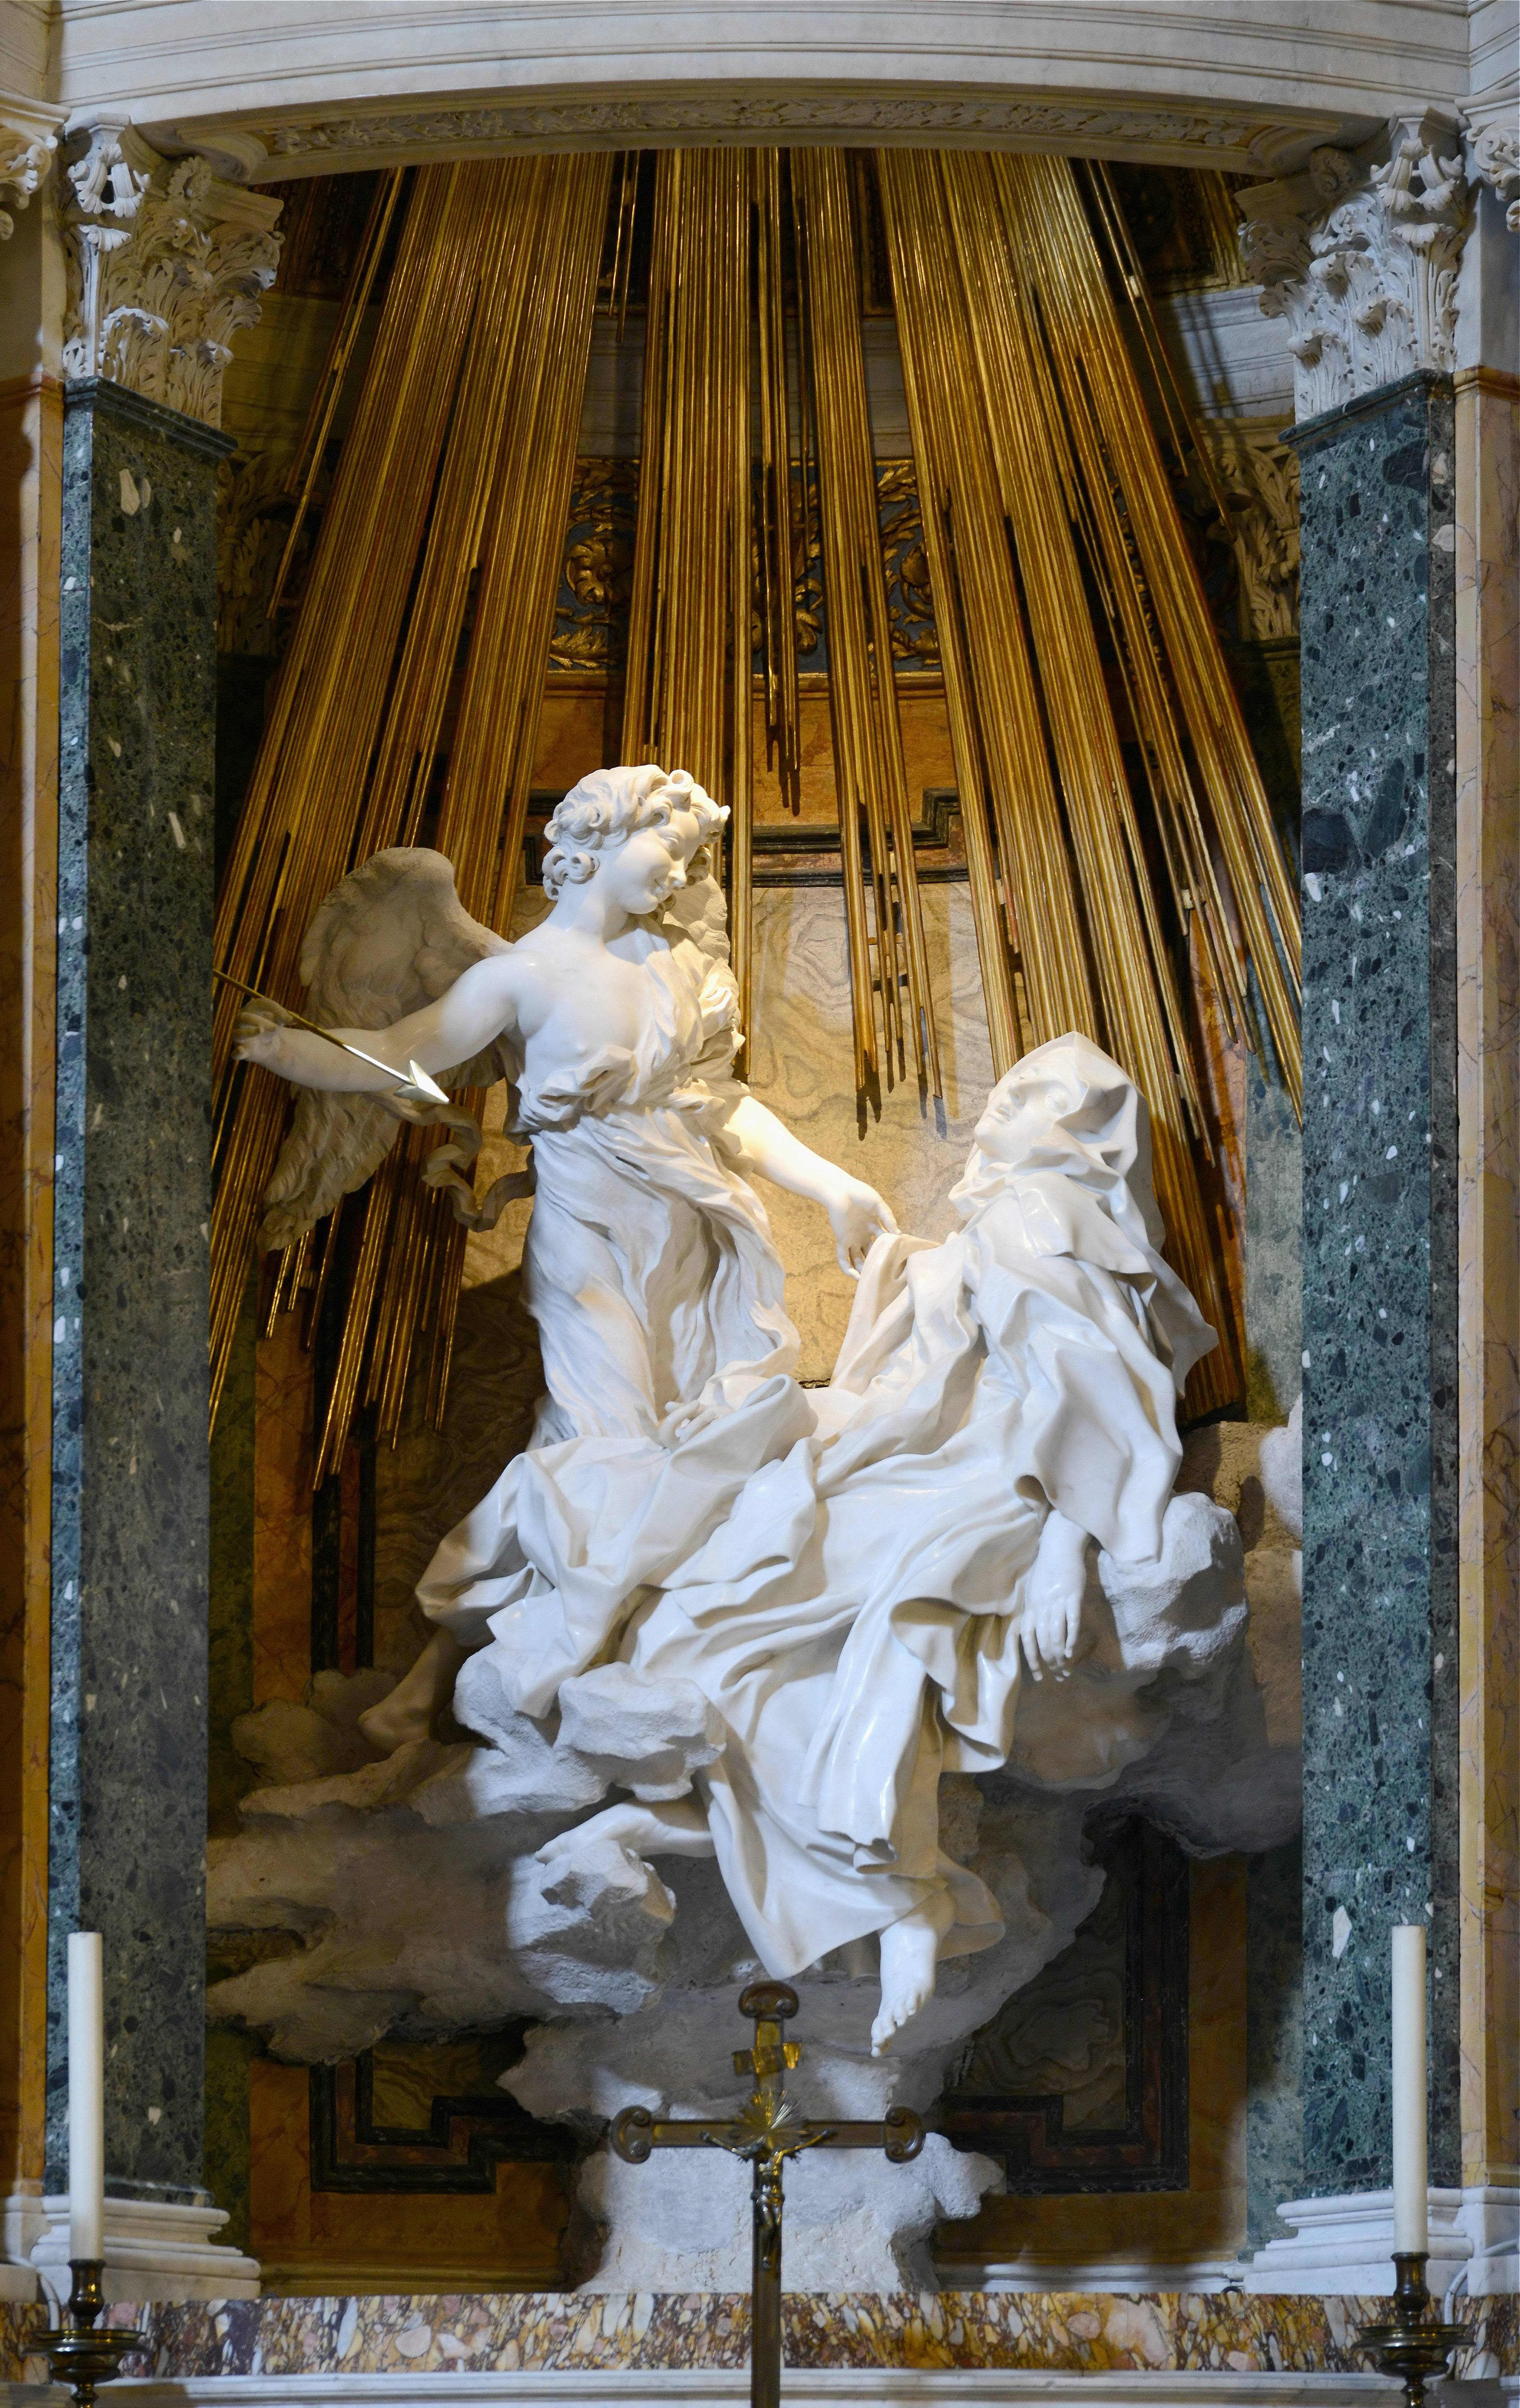
\includegraphics[width=4cm]{figura_9}
				\caption{\textit{O êxtase de Santa Teresa}, de Bernini.}
				\label{fig:mesh9}
			\end{figure}
			\par Lembre-se das visões de Santa Teresa expressas em seu diário. A dicotomia entre a lança do prazer e do sofrimento. Êxtase como forma de sensualização.
			\begin{figure}[h]
				\centering
				\includegraphics[width=4cm]{figura_10}
				\caption{\textit{Beata Ludovica Albertoni}, de Bernini.}
				\label{fig:mesh10}
			\end{figure}
			\par Novamente, um processo de sensualização.
			\begin{figure}[h]
				\centering
				\includegraphics[width=4cm]{figura_11}
				\caption{\textit{As três graças}, de Rafael (1483-1520) e Rubens (1577-1640).}
				\label{fig:mesh11}
			\end{figure}
			\par Compare a obra com a representação das três graças em \textit{Primavera}, de Botticelli, e note o maior enfoque na carnalidade e nas expressões faciais das mulheres.
			\par O pintor espanhol El Greco (1541-1614) também possui obras relevantes para nossos estudos. Em especial, em uma das pinturas representada abaixo, note a relação de Pedro e as chaves do céu, a presença de santos e anjos, imersos em um quadro saturado (dinâmico), com muitas informações visuais. O eixo ascensional (arte mundana) e os temas projetados.
			\begin{figure}[h]
				\centering
				\includegraphics[width=4cm]{figura_12}
				\caption{\textit{O enterro do Conde Orgaz}, de El Greco.}
				\label{fig:mesh12}
			\end{figure}
			\begin{figure}[h]
				\centering
				\includegraphics[width=4cm]{figura_13}
				\caption{\textit{A apoteose de Santo Inácio}, de Andrea Pozzo (1642-1709).}
				\label{fig:mesh13}
			\end{figure}
			\par Por fim, a obra em questão utiliza-se diretamente da noção de três dimensões e busca causar a sensação de ascendência do espectador.
			\par A arquitetura barroca, por sua vez, era elaborada e intrincada. Exemplos notáveis dessas construções são listados abaixo. É interessante notar, no caso da primeira imagem, a forma pela qual as escadarias construídas em zigue-zague atuam como desvios para a salvação do indivíduo.
			\begin{figure}[h]
				\centering
				\includegraphics[width=4cm]{figura_14}
				\caption{\textit{Santuário do Bom Jesus do Monte}, em Tenões, Portugal.}
				\label{fig:mesh14}
			\end{figure}
			\par O Barroco fora o estilo de época de maior duração. Ainda no Brasil, no final do século XVIII, tivemos o Barroco mineiro, tardio (enquanto a Europa vivia o Neoclassicismo, descrito na próxima parte). Haviam certas diferenças de material (preferência pela pedra sabão ao mármore), e a técnica de escorço também fora amplamente utilizada.
			\par \textbf{Carece de mais informações.}
			
			\chapter{A literatura barroca}
			\par Os dois principais estilos dessa época eram o \textbf{cultismo} e o \textbf{conceptismo}. De maneira geral, havia um contraste entre a vida terrena e a vida eterna, e a representação de Jesus era um símbolo para o conflito ideológico barroco, do lado humano que se sobressai durante a crucificação (Jesus frequentemente era representado crucificado, na figura de um mártir). Havia o uso recorrente de antíteses e paradoxos, antecipados pelo \textbf{Maneirismo}, no qual o escritor expressa as contradições de sua consciência. No capítulo, analisaremos em detalhes a obra de Gregório de Matos.
			
			\chapter{Gregório de Matos}
			\par Gregório de Matos (1636-1696) foi uma figura muito popular em vida, membro da elite de Salvador e de relações sanguíneas com a família portuguesa. Em uma época na qual os poemas eram passados de boca em boca, a tradição oral era muito presente na sociedade, e por isso existem muitas obras atribuídas\footnote{No século XIX teve início o primeiro esforço em compilar e organizar os seus poemas. Somente no século seguinte, no entanto, tal tarefa adquiriria um caráter mais sistemático e científico.} ao autor. Envolvido em diversas polêmicas (em especial, por suas poesias satíricas, na qual ridicularizava dos poderosos, ganhou a alcunha de \textbf{Boca do inferno}), Gregório teve de se exilar em Portugal.
			\par Em uma época na qual a Coroa proibia a impressão de poesias, e com uma taxa de alfabetização da população inferior a 10\%, a palavra oral é de grande relevância e influência (compare com uma situação de bullying, com linguagens refinadas e populares). Com isso, o autor tivera sua obra incorporada à cultura popular.
			\par Gregório produzira poesias em diversas vertentes:
			\begin{enumerate}
				\item \textbf{Poesia lírico-amorosa}, de caráter petrarquista\footnote{Lembre-se de Francesco Petrarca, um dos expoentes do Humanismo italiano. Com a obra \textit{Cancioneiro} e sua musa Laura, tornara-se um clássico moderno, estimulando a emulação (petrarquiana) por diversos autores (caracterizadas por elementos como metáforas e exaltação/sublimação da figura feminina). O célebre soneto de Camões, \textit{Alma minha gentil que te partiste}, constitui exemplo notável.}.
				\item \textbf{Poesia meditativa}, de temática filosófica.
				\item \textbf{Poesia devocional}, de temática religiosa.
				\item \textbf{Poesia encomiástica}, de elogio a uma figura pública. Note que, assim como a poesia satírica poderia acabar com a reputação de um indivíduo, a poesia encomiástica possuía o efeito contrário.
				\item \textbf{Poesia Satírica}, do gênero satírico (utilização do humor e do ridículo\footnote{Ridículo deriva do latim \textit{rides}, rir.} para criticar uma pessoa, grupo, instituição ou ideia (humor mordaz). Veja que o louvor e a sátira eram frequentemente aplicados a uma mesma figura pública, e constituem gêneros altamente convencionais, que variam de acordo com as circunstâncias. Ainda nesse sentido, note que os poemas nem sempre expressam o que o escritor pensa a respeito dos indivíduos, e que sátira e louvor não são conceitos necessariamente contrários (lembre-se do decoro: cada circunstância exige uma forma apropriada). Esse apontamento ficará mais claro adiante.
			\end{enumerate}
			\par Os poemas de Gregório apresentam, frequentemente, títulos longos, autoexplicativos, não necessariamente dados pelo autor. Em sua obra também se identificam tanto elementos conceptistas, como o braço do menino, o pecador sofista e o sol que não dura mais que um dia, assim como elementos cultistas, observados por meio de antíteses.
			\poemtitle{Buscando a Cristo}
			\settowidth{\versewidth}{Nessa cruz sacrossanta descobertos}
			\begin{verse}[\versewidth]
				A vós correndo vou, braços sagrados, \\
				Nessa cruz sacrossanta descobertos \\
				Que, para receber-me, estais abertos, \\
				E, por não castigar-me, estais cravados.

				A vós, divinos olhos, eclipsados \\
				De tanto sangue e lágrimas abertos\footnote{Cobertos, na edição de Sérgio Buarque de Holanda.}, \\
				Pois, para perdoar-me, estais despertos, \\
				E, por não condenar-me, estais fechados.
				
				A vós, pregados pés, por não deixar-me, \\
				A vós, sangue vertido, para ungir-me, \\
				A vós, cabeça baixa, p'ra chamar-me.
				
				A vós, lado patente, quero unir-me, \\
				A vós, cravos preciosos\footnote{Pregos (crucificação).}, quero atar-me, \\
				Para ficar unido, atado e firme. \\
			\end{verse}
			\par Os braços sagrados representam, por metonímia, a figura de Jesus na cruz. Há grande destaque para a misericórdia divina, com braços abertos para acolher o pecador e presos para condená-lo. Os divinos olhos de Jesus também expressam a antítese citada, e os pés pregados garantem que o pecador não será abandonado. Ao longo dos versos, novamente, observa-se o emprego de metonímias.
			\poemtitle{Moraliza o poeta nos Ocidentes do Sol a inconstância dos bens do mundo}
			\settowidth{\versewidth}{Depois da Luz se segue a noite escura,}
			\begin{verse}[\versewidth]
				Nasce o Sol, e não dura mais que um dia, \\
				Depois da Luz se segue a noite escura, \\
				Em tristes sombras morre a formosura, \\
				Em contínuas tristezas a alegria.
				
				Porém se acaba o Sol, por que nascia? \\
				Se é tão formosa a Luz, por que não dura? \\
				Como a beleza assim se transfigura? \\
				Como o gosto da pena assim se fia?
				
				Mas no Sol, e na Luz falte a firmeza, \\
				Na formosura não se dê constância, \\
				E na alegria sinta-se tristeza.
				
				Começa o mundo enfim pela ignorância, \\
				E tem qualquer dos bens por natureza \\
				A firmeza somente na inconstância. \\
			\end{verse}
			\par Utilização frequente de antíteses, e a construção da beleza como algo que se torna uma sombra à medida em que envelhece. Ocorrência de elipse com o verbo morrer. Não se pode esperar constância na beleza, e um dia a alegria tem um fim. Ideia de que a única coisa que nunca muda é o próprio fato de que as coisas mudam (inconstância como única constância). Identificamos o lugar-comum da \textbf{inconstância}, efemeridade: o indivíduo que aspira a eternidade (ob[rs]era?) a efemeridade da vida.
			\poemtitle{A Jesus Cristo nosso senhor}
			\settowidth{\versewidth}{Da vossa alta clemência me despido}
			\begin{verse}[\versewidth]
				Pequei, Senhor; mas não porque hei pecado, \\
				Da vossa alta clemência me despido\footnote{Despeço.}; \\
				Porque, quanto mais tenho delinquido, \\
				Vos tenho a perdoar mais empenhado.
				
				Se basta avos irar tanto pecado, \\
				A abrandar-vos sobeja um só gemido: \\
				Que a mesma culpa, que vos há ofendido, \\
				Vos tem para o perdão lisonjeado.
				
				Se uma ovelha perdida e já cobrada\footnote{Recuperada.} \\
				Glória tal e prazer tão repentino \\
				Vos deu, como afirmais na sacra história, 
				
				Eu sou, Senhor, a ovelha desgarrada, \\
				Cobrai-a; e não queirais, pastor divino, \\
				Perder na vossa ovelha a vossa glória. \\
			\end{verse}
			\par Ideia de que, quanto mais peco, mais Jesus se empenha em perdoar. Com um pecado, basta um gemido (dor e sofrimento) para ser perdoado. Construção do \textbf{sofismo} de que Jesus é gratificado com o pecado, em meio aos anseios do indivíduo que quer desfrutar dos prazeres terrenos, mas que ainda deseja a salvação. Se Jesus é capaz de perdoar o soldado de orelha perdida, também tem capacidade de perdoar o eu lírico. Contraste com a salvação em cada alma que não é salva.
			\poemtitle{Achando-se um braço perdido do Menino Deus de N. S. das Maravilhas, que desacataram infiéis na Sé da Bahia}
			\settowidth{\versewidth}{A parte sem o todo não é parte;}
			\begin{verse}[\versewidth]
				O todo sem a parte não é todo; \\
				A parte sem o todo não é parte; \\
				Mas se a parte o faz todo, sendo parte, \\
				Não se diga que é parte, sendo o todo. 
				
				Em todo a Sacramento está Deus todo, \\
				E todo assiste inteiro em qualquer parte, \\
				E feito em partes todo em toda a parte, \\
				Em qualquer parte sempre fica todo. 
				
				o braço de Jesus não seja parte, \\
				Pois que feito Jesus em partes todo, \\
				Assiste cada parte em sua parte.
				
				Não se sabendo parte deste todo, \\
				Um braço que lhe acharam, sendo parte, \\
				Nos diz as partes todas deste todo. 
			\end{verse}
			\par Construção de uma tautologia a partir de uma imagem quebrada. Deus se faz todo no rito da Eucaristia (Igreja e fiéis). O braço é um todo, e a parte, pois, é um todo (paradoxo).
			\poemtitle{À cidade da Bahia}
			\settowidth{\versewidth}{Estás e estou do nosso antigo estado!}
			\begin{verse}[\versewidth]
				Triste Bahia! ó quão dessemelhante \\
				Estás e estou do nosso antigo estado! \\ 
				Pobre te vejo a ti, tu a mi empenhado\footnote{Endividado.}, \\
				Rica te vi eu já, tu a mi abundante.
				
				A ti trocou-te\footnote{Duplo sentido, de comerciar e modificar. Indica a exploração da cidade de Salvador pelo comércio internacional, e a forma pela qual, a partir do Pacto Colonial, a riqueza da cidade é espoliada pelo mercado (inserção desfavorável do Brasil no sistema capitalista). Com efeito, Salvador exporta açúcar, de baixo valor agregado, e importa manufaturas, como tecidos.} a máquina mercante\footnote{Em referência às naus que aportavam para comerciar, símbolo do comércio internacional como um todo (reflexão sobre o capitalismo mercantil).}, \\
				Que em tua larga barra\footnote{Litoral, orla, praia (como em ``barra da calça''), limites da terra antes do mar.} tem entrado, \\
				A mim foi-me trocando, e tem trocado, \\
				Tanto negócio e tanto negociante.
				
				Deste em dar tanto açúcar excelente \\
				Pelas drogas inúteis, que abelhuda \\
				Simples\footnote{Simplório, ingênuo.} aceitas do sagaz\footnote{Esperteza, astúcia.} Brichote\footnote{Designação pejorativa dos ingleses. Lembre-se de que, desde o fim da União Ibérica, Portugal criara forte dependência da Inglaterra (note a relação Inglaterra $\Rightarrow$ Portugal $\Rightarrow$ Brasil).}.
				
				Oh se quisera Deus, que de repente \\
				Um dia amanheceras tão sisuda\footnote{Sagaz, astuta.} \\
				Que fora de algodão o teu capote! \\
			\end{verse}
		\par Por metonímia, Bahia é sinônimo para a cidade de Salvador. O eu lírico identifica a si mesmo e a população como muito diferentes do que um dia foram: no passado, a região era rica e o eu lírico, próspero. No entanto, agora a cidade está pobre e o eu lírico endividado, consequência das ações de negócios e negociantes. Lembre-se de que Gregório é ligado à elite produtora de açúcar. Assim, inserido no contexto da emergência de uma nova elite baseada no comércio internacional, ele, da elite tradicional, começa e se endividar. Com efeito, as principais riquezas já não estavam mais relacionadas ao açúcar, mas ao tráfico de escravos. Além disso, os mesmos indivíduos que executavam tal prática também concediam empréstimos de dinheiro.
		\par Por todo o soneto, é evidente o sentimento de \textbf{desqualificação social}, a perda de prestígio social e poder econômico da classe da qual Gregório fazia parte, aliado a um \textbf{ressentimento social}, rancor. Na visão do autor, ele, por ser um fidalgo, deveria ser o detentor do prestígio, e não uma nova elite, muitas vezes de origem mestiça, nas classes trabalhadoras (visão racista acerca da sociedade brasileira). Ao fim, Gregório descreve o fato de que o algodão era menos caro do que o linho inglês (símbolo de status), e espera que um dia a colônia perceba que não precisa do tecido da Inglaterra, pois já possui o algodão.
		\poemtitle{Contemplando nas cousas do mundo desde o seu retiro, the atira com o seu ápage, como quem a nado escapou da tormenta}
		\settowidth{\versewidth}{Quem mais limpo se faz, tem mais carepa;}
		\begin{verse}[\versewidth]
			Neste mundo é mais rico o que mais rapa\footnote{Rouba.}: \\
			Quem mais limpo se faz, tem mais carepa\footnote{Caspa, sujeira do cabelo. Neste caso, quem se diz honesto é o mais corrupto.}; \\
			Com sua língua, ao nobre o vil decepa\footnote{O nobre cai nas mãos dos mal-intencionados. O vil fala mal dos bons, mas deveria ocorrer o contrário. Note a catacrese presente no termo \textit{vil}.}: \\
			O velhaco maior sempre tem capa\footnote{Indumentária, símbolo de status social utilizada pelos nobres (velhaco maior). Nesse contexto, quem tem prestígio social são os enganadores, que o conquistam por meio de manipulações.}.
			
			Mostra o patife da nobreza o mapa\footnote{Exibe genealogia, pretende-se descendente de linhagem nobre. Mapas genealógicos eram frequentemente falsificados.}: \\
			Quem tem mão de agarrar, ligeiro trepa\footnote{Ascende socialmente.}; \\
			Quem menos falar pode, mais increpa\footnote{O mais corrupto é o que mais reclama da corrupção.}: \\
			Quem dinheiro tiver, pode ser Papa\footnote{Para ser Papa, não é preciso ser virtuoso. Apenas dinheiro é necessário (o cargo de Papa como metonímia para qualquer cargo da sociedade).}. 
			
			A flor baixa\footnote{Rasteira, comum.} se inculca por tulipa\footnote{Ornamental, reconhecida pela beleza.}; \\
			Bengala hoje na mão, ontem garlopa\footnote{Metonímias da condição social, opostas ironicamente: hoje \textit{bengala}, índice de fidalguia, ontem \textit{garlopa}, ferramenta de marcenaria, para aplainar madeira grossa, índice do trabalho braçal (mal visto, sobretudo em uma nação escravista, que contamina tais ofícios com estigmas).}: \\
			Mais isento se mostra o que mais chupa\footnote{Puxar o saco de alguma figura (são as pessoas mais interesseiras e que se proveitam das outras).}.
			
			Para a tropa do trapo\footnote{Preconceito com a classe trabalhadora.} vazo a tripa\footnote{Tem o sentido de defecar. Manifestação máxima de desprezo pela ``tropa do trapo'', i.e., a fidalguia baiana sem tradição. Nota-se, também, o emprego da paranomásia, trocadilho com a proximidade sonora dos termos do verso.}, \\
			E mais não digo, porque a Musa\footnote{Inspiram o trabalho artístico e poético.} topa \\
			Em apa, epa, ipa, opa, upa\footnote{Combinação difícil de palavras. Veja que, nesse verso, Gregório transpassa a ideia de que encerrara o soneto pois já mostrara sua capacidade em rimar com ``apa, epa, ipa, opa, upa'', e poderia continuar até quando quisesse.}. 
		\end{verse}
		\par No soneto, Gregório evidencia que aqueles que detêm o \textbf{capital cultural}, o conhecimento, são eles, a elite. Identificamos o lugar-comum (tema recorrente na tradição literária) do \textbf{mundo às avessas}\footnote{Lembre-se, nesse sentido, de falas como ´´bom mesmo era na minha época''.}, em que os valores foram invertidos na sociedade. Veja, no entanto, que o autor não chega a um lugar-comum mais extremo, grotesco, mas se apropria desse tema da tradição para dar-lhe um significado específico relacionado ao seu contexto social, no qual a sua classe de origem, a elite tradicional dos proprietários de terra, perde o prestígio social e a força econômica.
		\par Um apontamento realizado ao longo da análise reside nas diferentes facetas do \textbf{capital}, seja ele social ou econômico, por exemplo. Ao estudarmos o Naturalismo e, em especial, Aluísio Azevedo (1857-1913), tais temas serão aprofundados.
		\poemtitle{Ao mesmo assunto}
		\settowidth{\versewidth}{Camisa de urucu, mantéu de arara,}
		\begin{verse}[\versewidth]
			Um calção de pindoba\footnote{Palmeira, coqueiro.}, a meia zorra\footnote{Péricles Eugênio da Silva Ramos supõe caindo.}, \\
			Camisa de urucu\footnote{O corpo pintado de vermelho, com a tinta do fruto.}, mantéu de arara, \\
			Em lugar de cotó\footnote{Espada curta.}, arco e taquara, \\
			Penacho de guarás, em vez de gorra.
			
			Furado o beiço, e sem temor que morra \\
			O pai, que lho envasou cuma titara\footnote{Nome de palmeira, aqui vareta.}, \\	
			Porem a Mãe a pedra lhe aplicara \\
			Por reprimir-lhe o sangue que não corra.
			
			Alarve\footnote{Tolo, burro, imbecil.} sem razão, bruto sem fé\footnote{Não possui o refinamento da religião, sem leis.}, \\
			Sem mais leis que a do gosto, quando erra, \\
			De Paiaiá tornou-se em abaité\footnote{Gente feia, repelente.}.
			
			Não sei onde acabou, ou em que guerra: \\
			Só sei que deste Adão de Massapé\footnote{Forma de construção tipicamente indígena.} \\ 
			Procedem os fidalgos desta terra. 
		\end{verse}
		\par Um aspecto relevante do estilo poético de Gregório, e que mais o diferencia dos outros autores do período barroco, é a incorporação de termos com origens indígena e africana (língua brasílica). Por essa razão, podemos erroneamente concluir que era um escritor protonacionalista, que talvez demonstrasse a cultura nacional em detrimento da europeia. Diversos são os motivos que invalidam tal apontamento.
		\par Primeiramente, veja que o poema não é muito prestigioso, utilizando-se de superstições acerca da cultura desses povos, além de termos como ``meia-zorra'' e ``taquara'' em contextos depreciativos. Ademais, note que Gregório não utilizara termos de tais culturas fora do gênero satírico. Ocorre que o escritor se apropriara destes termos para rebaixar e ridicularizar, neste caso, a cultura indígena local. Por fim, ao não valorizá-los e, pelo contrário, denegri-los\footnote{Termo antigo, de origem no latim \textit{denigrare}, manchar a reputação.}, insinua que a nova elite brasileira, proveniente desses povos, também é ignorante e selvagem.
		\par Títulos como esse são comuns na obra de Gregório de Matos. Para evitar confusões, considere que o poema reproduzido acima é o segundo seguinte ao soneto \textit{Aos principais da Bahia chamados os caramurus}.
		\poemtitle{Disparates na língua brasílica a huma cunhaã, que ali galanteava por vicio}
		\settowidth{\versewidth}{encontrei Quatimondé}
		\begin{verse}[\versewidth]
			Indo à caça de tatus \\
			encontrei Quatimondé \\
			na cova de um jacaré \\
			tragando trezes Teiús: \\
			eis que dous Surucucus \\
			como dous Jaratacacas\\
			vi vir atrás de umas Pacas,\\
			e a não ser um Preá \\
			creio, que o Tamanduá \\
			não escapa às Gebiracas.
			
			De massa um tapiti, \\
			um cofo de Sururus, \\
			dous puçás de Baiacus, \\
			Samburá de Murici: \\
			Com uma raiz de aipi \\
			vos envio de Passé, \\
			e enfiado num imbé \\
			Guiamu, e Caiaganga, \\
			que são de Jacaracanga \\
			Bagre, timbó, Inhapupê.
			
			Minha rica Cumari, \\
			minha bela Camboatá \\
			como assim de Pirajá \\
			me desprezas tapiti: \\
			não vedes, que murici \\
			sou desses olhos timbó \\
			amante mais que um cipó \\
			desprezado Inhapupê, \\
			pois se eu fora Zabelê \\
			vos mandara um Miraró.
		\end{verse}
		\par Disparate é algo absurdo. Cunhaã, por sua vez, em tupi-guarani, significa moça, mulher jovem. Galanteava (cortejava, namorava) por vício (qualidade imoral, antônimo de virtude, comportamento reprovável). Nesse caso, o namoro imoral de uma jovem refere-se à prostituição com uma indígena.
		\par Logo no início do poema, é notória a extensa referência a animais como tamanduás, aves e serpentes. Note, também, que a dualidade (oposição de valores) da preocupação com a vida após a morte e o apego aos prazeres da vida também se fazem presentes nos escritos do autor.
		\par Além disso, também identificamos uma dualidade entre a poesia lírico-amorosa e erótica produzidas por Gregório: de um lado temos uma poesia lírico-amorosa petrarquista, caracterizada pela exaltação e sublimação da figura feminina, destinada às mulheres caucasianas e de classe social elevada; por outro lado, verificamos uma poesia de baixo estilo (palavras de baixo calão, erotização), com apelo fortemente carnal, de caráter até mesmo pornográfico, destinada às mulheres de origem indígena e africana, assim como às mestiças (a \textit{tropa do trapo}).
		\poemtitle{Juízo anatômico dos achaques que padecia o corpo da República, em todos os membros, e inteira definição do que em todos os tempos é a Bahia}
		\begin{verse}
			1 \\
			Que falta nessa cidade? \dotfill Verdade. \\
			Que mais por sua desonra? \dotfill Honra. \\
			Falta mais que se lhe ponha? \dotfill Vergonha.
			
			\hspace{5em} O demo a viver se exponha, \\
			\hspace{5em} Por mais que a fama a exalta, \\
			\hspace{5em} Numa cidade onde falta \\
			\hspace{5em} Verdade, honra, vergonha. 
			
			2 \\
			Quem a pôs neste socrócio\footnote{Afrânio Peixoto grafa \textit{rocrócio}. Em um dos apógrafos vem \textit{socrócio}. Na primeira hipótese, retrocesso. Na segunda hipótese, socrócio, criado por necessidade de eco com negócio, de socrestar, furtar, rapinar.}? \dotfill Negócio\footnote{Colocou Salvador na situação em que se encontra.}. \\
			Quem causa tal perdição? \dotfill Ambição\footnote{Ganância, desejo de possuir tudo.}. \\
			E a maior desta loucura? \dotfill Usura\footnote{Termo já citado no capítulo de introdução ao Barroco, envolve o processo de empréstimo de dinheiro e sequente cobrança de juros. Era condenada pela Igreja Católica e, em muitas nações, considerada um crime. Max Weber, nesse contexto, descreve que os judeus foram associados ao dinheiro pois realizavam empréstimos com as leis restritivas de aquisição de bens fundiários. Foram descriminados, sobretudo na Europa, pois foram os assassinos de Cristo ao escolherem libertar Barrabás. Relembre \textit{O mercador de Veneza}, de Shakespeare. Gregório associa a usura à elite mercantil emergente (falta de verdade, honra e vergonha causada pelo negócio, ambição e usura).}.
			
			\hspace{5em} Notável desaventura \\
			\hspace{5em} De um povo néscio, e sandeu, \\
			\hspace{5em} Que não sabe que o perdeu \\
			\hspace{5em} Negócio, ambição, usura.
			
			3 \\
			Quais são os seus doces objetos? \dotfill Pretos. \\
			Tem outros bens mais maciços? \dotfill Mestiços. \\
			Quais destes lhe são mais gratos? \dotfill Mulatos.
			
			\hspace{5em} Dou ao demo os insensatos, \\
			\hspace{5em} Dou ao demo a gente asnal\footnote{Burro}, \\
			\hspace{5em} Que estima por cabedal\footnote{Riqueza.} \\
			\hspace{5em} Pretos, mestiços, mulatos\footnote.
			
			4 \\
			Quem faz os círios mesquinhos? \dotfill Meirinhos. \\
			Quem faz as farinhas tardas? \dotfill Guardas. \\
			Quem as tem nos aposentos? \dotfill Sargentos.
			
			\hspace{5em} Os círios lá vêm aos centos, \\
			\hspace{5em} E a terra fica esfaimando \\
			\hspace{5em} Porque os vão atravessando \\
			\hspace{5em} Meirinhos, guardas, sargentos.
			
			5 \\
			E que justiça a resguarda?  \dotfill Bastarda. \\
			É grátis distribuída? \dotfill Vendida. \\
			Que tem, que a todos assusta? \dotfill Injusta. 
			
			\hspace{5em} Valha-nos Deus, o que custa \\
			\hspace{5em} O que El-Rei nos dá de graça, \\
			\hspace{5em} Que anda a justiça na praça \\
			\hspace{5em} Bastarda, vendida, injusta. 
			
			6 \\
			Que vai pela clerezia? \dotfill Simonia. \\
			E pelos membros da Igreja? \dotfill Inveja. \\
			Cuidei que mais se lhe punha? \dotfill Unha\footnote{Nesse contexto, com o sentido de roubalheira.}.
			
			\hspace{5em} Sazonada caramunha\footnote{Experimentada lamentação (Amora).} \\
			\hspace{5em} Enfim, que na Santa Sé \\
			\hspace{5em} O que mais se pratica é \\
			\hspace{5em} Simonia, inveja, unha.
			
			7 \\
			E nos frades há manqueiras\footnote{Claudicação. No texto, deslize moral.}? \dotfill Freiras. \\
			Em que ocupam os serões? \dotfill Sermões. \\
			Não se ocupam em disputas? \dotfill Putas.
			
			\hspace{5em} Com palavras dissolutas \\
			\hspace{5em} Me concluís, na verdade, \\
			\hspace{5em} Que as lidas todas de um Frade\\
			\hspace{5em} São freiras, sermões, e putas.
			
			8 \\
			O açúcar já se acabou? \dotfill Baixou\footnote{Queda dos preços desse produto no mercado.}. \\
			E o dinheiro se extinguiu? \dotfill Subiu\footnote{Aumento dos juros.}. \\
			Logo já convalesceu? \dotfill Morreu\footnote{Em relação à economia. Revela preocupação material com sua classe de origem.}.
			
			\hspace{5em} À Bahia aconteceu \\
			\hspace{5em} O que a um doente acontece, \\
			\hspace{5em} Cai na cama, o mal lhe cresce, \\
			\hspace{5em} Baixou, subiu, e morreu.
			
			9 \\
			A Câmara não acode? \dotfill Não pode. \\
			Pois não tem todo o poder? \dotfill Não quer. \\
			É que o governo a convence? \dotfill Não vence.
			
			\hspace{5em} Quem haverá que tal pense, \\
			\hspace{5em} Que uma Câmara tão nobre, \\
			\hspace{5em} Por ver-se mísera e pobre, \\
			\hspace{5em} Não pode, não quer, não vence. 
		\end{verse}
		\par Gregório de matos trata a Bahia como um corpo, organismo vivo, atuando, nesse sentido, como um médico que analise o caso. Há uma estrutura fixa de tercetos seguidos de quartetos, com estrofes de três versos em redondilha maior (sete sílabas poéticas). Nos quartetos se retoma as palavras de complemento dos tercetos.
		\par Para o escritor, um dos problemas de Salvador é que se valoriza uma população de pretos, mestiços e mulatos. Além disso, insinua que as ocupações de um padre da cidade são freiras, sermões e prostitutas (hipocrisia).
		\par Baixou (açúcar) para a cama, a febre subiu (juros) e morreu (economia).
		
	\part{Neoclassicismo}
	
		\chapter{Introdução}
		\par O \textbf{Iluminismo} foi um movimento filosófico de contestação dos modelos ideológicos vigentes (tradicionais), pautado no \textbf{racionalismo}. Contestação pois, até o chamado Século das Luzes, o conhecimento ocidental estava baseado no tripé \textbf{fé}, \textbf{autoridade} e \textbf{tradição}.
		\par Para a fé, existem questões que o indivíduo não precisa entender para assumir como verdade, pois são da ordem do divino (relevadas pela Bíblia, e não encontradas pela razão - estão além da compreensão humana). Assim sendo, resta aos mortais apenas aceitá-las (lembre-se da frase de Santo Agostinho, em relação à Santíssima Trindade: \textit{Credo quia absurdum}, creio porque é absurdo.). Note que fé é diferente de crença: esta representa o conjunto de ideias e dados que falam sobre a realidade e que o indivíduo assume como possíveis ou prováveis, ao passo que a fé é uma crença no que não pode ser provado, por definição, mesmo sem nenhuma comprovação e mesmo no impossível. Há coisas na Bíblia que precisam ser aceitas pois são revelações de Deus, ainda que não sigam a razão humana.
		\par Autoridades são figuras recobertas de tradição e fontes privilegiadas da verdade (relembre de Aristóteles que, no livro \textit{Historia animalium}, classificara as aranhas como insetos).
		\par Para a tradição, algo é verdade pois os indivíduos sempre acreditaram nisso. Envolve práticas e costumes que se repetem ao longo da história, como o casamento entre homens e mulheres (tais ideias possuem mais credibilidade do que aquelas que surgem recentemente). Um exemplo notável é a história de Galileu Galilei, que demonstrara que a Terra não era o centro do Universo e fora não só questionado por diversos outros astrônomos do período, como também investigado pela Inquisição. Veja que, para o Iluminismo, as ideias devem ser validadas por meio da razão (comprovação da veracidade), i.e., a razão empregada individualmente é o critério máximo de validação da verdade, subordinando até mesmo a fé, a autoridade e a tradição.
		\par Para o filósofo Immanuel Kant, o \textbf{esclarecimento} se baseia na saída da minoridade intelectual - quando outros indivíduos determinam no que se deve acreditar - e a entrada na maioridade - formação das próprias ideias pelo uso da razão.
		\par O Iluminismo se contrapõe aos fundamentos ideológicos do antigo regime, pois estes se baseavam, especialmente, na tradição e religião (o monarca representa o Estado e pode estabelecer a lei como bem desejar, tendo ainda o poder de decisão da vida e morte dos súditos). O que garantiria que determinado indivíduo seria o melhor governante, ou por que se deveria depositar confiança em sua autoridade? Até então, a resposta para tais questionamentos era simples: Deus o colocou ali (a religião justifica a existência do Absolutismo). Com a dúvida da providência divina, tais respostas também começam a ser questionadas.
		\par Em relação ao aspecto supracitado, é válida a análise do Baruch Espinoza: Deus criou o mundo, é onisciente, onipotente e onipresente. Não podemos, pois, esperar menos do que a perfeição das leis da natureza. No entanto, dessa forma os milagres não poderiam existir, pois o mundo não seria perfeito. A conclusão é de que ou Deus é onisciente, onipresente e onipotente, ou os milagres existem. Também o filósofo francês René Descartes, que, pensando em seus pensamentos em frente a uma fogueira, tinha a única certeza de que ``Penso, logo existo'': todas as ideias devem ser questionadas e provadas racionalmente (falsidade da tradição).
		\par Nesse período, também se deflagraram as revoluções liberais, que alcançaram o ápice com a Revolução Francesa, na Europa, a qual iniciara um regime moderno simbolizado pela decapitação do monarca.
		\par É nesse contexto em que surge o Neoclassicismo, uma retomada dos valores estéticos e mitológicos do Classicismo (este, por sua vez, uma retomada dos valores estéticos da Antiguidade Clássica, a cultura greco-romana), como o equilíbrio, proporção, simetria, racionalidade, hedonismo, etc.
		\par O compositor austríaco Wolfgang Amadeus Mozart foi o maior representante da música neoclássica, referida brevemente como classicista. De maneira geral, Neoclassicismo é o termo que o estilo de época vai adquirir em todas as áreas, ao passo que Arcadismo é o termo que o Neoclassicismo assume na Literatura.
		\par Arcadia era um região montanhosa localizada na Grécia que, na Antiguidade, era conhecida pela atividade pastoril (pecuária). Por muito tempo, os gregos acreditavam que era a região mais antiga da Grécia, e de onde se originou (\textit{arcadia}, origem).
		
		\chapter{A literatura arcadista}
		\par A principal caraterística do Arcadismo é a emulação de um tipo de poesia pastoril realizada na Roma Antiga - as \textbf{éclogas} -, uma forma do gênero lírico no qual o eu lírico se passa por um pastor (poesia bucólica\footnote{Bucolismo é a abordagem do campo como um espaço de beleza e tranquilidade, onde é possível entrar em harmonia com a natureza e encontrar felicidade.}, de temática pastoril). Écloga, ou égloga, é uma forma da poesia lírica romana da Antiguidade de temática pastoril e amorosa. Novamente, retornamos à emulação: a cópia dos clássicos, que possuem os valores universais, neste caso, oriundos da Antiguidade.
		\par Um aspecto comum dessas produções é a \textbf{ambientação campestre}, na qual o eu lírico, geralmente um pastor com pseudônimo latino (como o caso de Tomás Antônio Gonzaga, que adotara o pseudônimo de Dirceu), que se declara apaixonado por uma \textit{nise} (pastora). A \textbf{idealização da vida no campo} também se faz presente. Lembre-se, afinal, de que a vida dos camponeses na Europa - e também em Roma, na Antiguidade - do século XVIII era difícil. Com efeito, as éclogas refletiam, sobretudo a visão dos senhores que as escreviam ou as encomendavam.
		\par Por fim, outra característica importante a ser mencionada é o \textbf{idílio}: a representação de uma vida amorosa feliz em contato com a natureza. No Trovadorismo português havia o coito amoroso e, no Classicismo, o amor tirano (como o caso de Inês de Castro), na poesia romana havia a visão de uma vida amorosa feliz). Cabe apenas pontuar que identificamos, em alguns casos, a representação da saudade, da expectativa da volta da amada e, em raras ocasiões, poemas que representam o amor como algo negativo, mas a visão é predominantemente idílica.
		\par Alguns lugares-comuns merecem maior atenção. São eles:
		\begin{enumerate}
			\item \textit{Carpe diem}: colha o dia, aproveite o momento presente.
			\item \textit{Locus amoenus}: lugar aprazível, descrição da paisagem do campo com ênfase para a beleza da natureza e para a tranquilidade.
			\item \textit{Fugere urbem}: fugir da cidade, a cidade como o palco das paixões humanas, onde o indivíduo vive umam vida tribulada e ilusória, baseada no luxo e na vaidade (pronúncia incerta do latim).
			\item \textit{Aurea mediocritas}: medida de ouro, o indivíduo, para ser feliz, deve buscar o caminho do meio, o equilíbrio: não deve ser muito pobre nem rico, deve ter uma vida simples.
			\item \textit{Inutilia truncat}: cortar o inútil, tudo aquilo que não é essencial deve ser dispensado. Ater-se ao que for essencial e dispensar o que for supérfluo. Aplicado na expressão poética, sugere que o estilo deve ser simples, sem excesso de figuras de linguagem (uma crítica aos excessos da literatura barroca, que entre os séculos XVII e XVIII, passou a ser considerada algo exacerbado).
		\end{enumerate}
		\par A poesia árcade era escrita para a elite aristocrática, em um período de transição da aristocracia para a burguesia que, à medida em que é reprimida, deseja se afugentar nos campos, fugir das cidades onde a burguesia enriquece e a população se revolta. É a negação de uma sociedade muito mais dinâmica que surge para formar a burguesia do século XVIII.
		\poemtitle{Convite a Marília}
		\settowidth{\versewidth}{Envolto nos seus úmidos vapores}
		\begin{verse}[\versewidth]
			Já se afastou de nós o inverno agreste\footnote{Sem chuva.} \\
			Envolto nos seus úmidos vapores\footnote{Névoa, neblina formada em situações de baixa temperatura.}; \\
			A fértil primavera, a mãe das flores, \\
			O prado\footnote{Forma de relevo.} ameno de boninas\footnote{Flor do campo.} veste.
			
			Varrendo os ares, o sutil Nordeste\footnote{Vento que sopra do nordeste.} \\
			Os torna azuis\footnote{Céu azul, sem nuvens.}; as aves de mil cores \\
			Adejam\footnote{Bater as asas.} entre Zéfiros\footnote{Relembre a pintura de Botticelli. Zéfiros representa o vento oriental, e Bóres, o ocidental.} e Amores\footnote{Cupido.}, \\
			E toma o fresco Tejo\footnote{Localizado em Portugal.} a cor celeste\footnote{Por reflexão da superfície.}.
			
			Vem, ó Marília, vem lograr comigo \\
			Destes alegres campos a beleza, \\
			Destas copadas árvores o abrigo.
			
			Deixa louvar da corte\footnote{Espaço onde os nobres se reúnem em torno do rei (Corte Real). Na poesia, torna-se sinônimo da sede do reinado de Portugal, localizada em Lisboa, a maior cidade. De maneira geral, serve de metonímia para uma grande cidade, principal.} a vã\footnote{Algo passageiro, ilusório, que não levará a nada.} grandeza: \\
			Quanto me agrada mais estar contigo \\
			Notando as perfeições da Natureza!
		\end{verse}
		\par Há a presença do lugar-comum \textit{locus amoenus}, em especial na descrição das árvores com copa como abrigo e sombra. Além disso, A vida de luxo das cidades é tratada como vã, em oposição com a vida no campo, permeada pelas perfeições da natureza (\textit{fugere urbem}).
		
		\chapter{Arcadismo em Portugal}
		\par Formação do mecenato lusitano. Marquês de Pombal, um dos ministros de Dom João V. Expulsou os jesuítas no contexto da educação ligada à escolástica, e era um símbolo do despotismo esclarecido.
		\par Déspota é um governante autoritário, tirano, que centraliza o poder. Esclarecido deriva de esclarecimento, descrito no capítulo de introdução da seção, aquele que se utiliza do poder de forma racional, buscando a liberdade e a igualdade. Kant os referiu com o monarca da Áustria, que era como um patrono dos filósofos.
		\par A Arcadia lusitana recebia incentivo fiscal de Pombal, o qual também recebera poemas encomiásticos destinados a sua figura.
			\section{Manuel du Bocage}
			\par Um poeta árcade português. Produzira poemas líricos, pornográficos e outros, em geral, racistas. É interessante mencionar que, embora possua uma vertente de acordo com os valores do Arcadismo, é possível identificar em parte de suas obras elementos do Romantismo, estilo de época posterior (\textit{pré-romantismo}\footnote{Incorporação de elementos pessoais e informações biográficas - como experiências pessoais e vivências - na poesia lírica, afastando-se, por vezes, dos convencionalismos da poesia árcade.}).
			\par O Classicismo e o Neoclassicismo foram estilos de época muito convencionais. De maneira geral, o poeta lírico era habilidoso em se utilizar dos lugares-comuns e emular os clássicos, além de fazer bom uso do decoro. Tome como exemplo o soneto de Camões \textit{Alma minha gentil que te partiste}, assim como a figura da amante Inês de Castro: não devemos assumir que o autor estava expressando verdadeiramente os seus sentimentos e a sua vida, pois se valorizava convencionalismo, e não autenticidade. A concepção de que a poesia lírica expressava sentimentos honestos surgiria apenas no Romantismo.
			\par É um dos poetas mais representativos do Arcadismo português.
			\poemtitle{Soneto do Epitaphio}
			\settowidth{\versewidth}{Mais um daqueles, que não fazem falta,}
			\begin{verse}[\versewidth]
				Lá quando em mim perder a humanidade \\
				Mais um daqueles, que não fazem falta, \\
				Verbi-gratia — o theologo, o peralta, \\
				Algum duque, ou marquez, ou conde, ou frade:
				
				Não quero funeral communidade, \\
				Que engrole sub-venites\footnote{Canto em intenção dos mortos.} em voz alta; \\
				Pingados gatarrões, gente de malta\footnote{Do povo, sem importância.}, \\
				Eu também vos dispenso a caridade:
				
				Mas quando ferrugenta enchada idosa \\
				Sepulchro me cavar em ermo outeiro, \\
				Lavre-me este epitaphio\footnote{Escrito colocado na lápide.} mão piedosa:
				
				«Aqui dorme Bocage, o putanheiro: \\
				Passou vida folgada, e milagrosa; \\
				«Comeu, bebeu, fodeu sem ter dinheiro.
			\end{verse}
			\par Trata-se de um poema auto-satírico, no qual o autor é o próprio alvo das ironias e críticas. Insinua que, quando morrer, não fará falta para os outros. Revela não desejar nenhum duque, marquez, conde ou frade em seu funeral, tampouco gente de malta.
			\par Fato curioso é que Bocage também escrevera um soneto satirizando o próprio nariz, \textit{Nariz, nariz e nariz}.
			
		\chapter{Arcadismo no Brasil}
		\par A Arcadia mineira era localizada em Vila Rica (atual Ouro Preto), sobretudo em razão do Ciclo do Ouro e, mais especificamente, durante sua decadência (nesse período, a prata chegou a ser mais valiosa do que o próprio ouro, dada a tamanha oferta). Surgimento de uma elite extremamente rica, cujos filhos estudavam na Universidade de Coimbra e, posteriormente, retornavam ao Brasil, onde atuavam como juízes e em outros cargos. Sofriam influência de ideias iluministas, refletidas na Conjuração Mineira.
		\par A Inconfidência Mineira tivera claras influências iluministas, e contara com a participação de diversos poetas árcades. Ocorrerera no contexto do declínio da produção de ouro e da criação das casas de fundição - as quais proporcionaram uma maior cobrança de impostos. O grupo fora delatado por José Silvério dos Reis. É curioso mencionar que o atual Museu da Inconfidência era uma prisão, onde aqueles que cometeram delitos esperavam o julgamento (destaque para penas mais duras, rígidas, após a Conjuração).
		\par Ouro Preto foi o principal centro difusor do Neoclassicismo, por meio de jovens que estudavam em Coimbra e retornavam com ideias iluministas (muitos participaram da Inconfidência Mineira).
			\section{Cláudio Manuel da Costa}
			\par Foi um dos poetas árcades mais velhos. Interessou-se pela poesia por meio do Barroco, fato presente em sua obra por meio do \textbf{barroquismo} - sobrevivência de elementos barrocos na poesia árcade o autor.
			\poemtitle{Leia a posteridade, ó pátrio Rio}
			\settowidth{\versewidth}{Em meus versos teu nome celebrado,}
			\begin{verse}[\versewidth]
				Leia a posteridade\footnote{Gerações futuras.}, ó pátrio Rio\footnote{Ribeirão do Carmo, que corta a cidade de Mariana.}, \\
				Em meus versos teu nome celebrado, \\
				Porque vejas uma hora despertado \\
				O sono vil do esquecimento frio:
				
				Não vês nas tuas margens o sombrio, \\
				Fresco assento de um álamo\footnote{Árvore encontrada no hemisfério norte.} copado; \\
				Não vês Ninfa cantar, pastar o gado \\
				Na tarde clara do calmoso estio.
				
				Turvo banhando as pálidas areias \\
				Nas porções do riquíssimo tesouro \\
				O vasto campo da ambição recreias.
				
				Que de seus raios o Planeta louro\footnote{Sol. No sistema astronômico geocêntrico, o planeta dourado. Utilização de perífrase, característica comum ao Barroco.}, \\
				Enriquecendo o influxo em tuas veias, \\
				Quanto em chamas fecunda, brota em ouro.
			\end{verse}
			\par No poema, o autor descreve o pátrio Rio em referência ao Ribeirão do Carmo, que corta a cidade de Mariana - a primeira cidade, capital e arquidiocese de Minas Gerais. Menciona o ouro de aluvião tão procurado em suas margens, então degradadas e sem a proteção de matas ciliares.
			\par Descreve que, para que o rio não seja esquecido pela posteridade, deve ser registrado. Lugar-comum da \textbf{imortalidade da memória} (herói de Homero) e \textit{kleos} (a poesia permitia que os indivíduos se lembrassem dos acontecimentos).
			\par Cláudio descreve que, nas margens do Ribeirão do Carmo, não há álamos que forneçam sombra e descanso. Não há ninfas cantando ou gado pastando da tarde clara do inverno. Também não há pasto, justamente pela atividade econômica desenvolvida na região. \textbf{As convenções da poesia árcade europeia não se enquadram no cenário de Mariana/Vila Rica}.
			\par Há a negação do lugar-comum \textit{locus amoneus}, à medida em que é necessário se afastar das convenções do Arcadismo (clima mediterrâneo) para descrever a região. Tal processo, referido como \textbf{nativismo}, ocorre quando o poeta fala sobre a realidade local em vez de, por exemplo, de um campo idealizado (cenário bucólico). Incorporação da cor local. O Ribeirção do Carmo não pode ser descrito por meio do \textit{locus amoenus}, em paralelo com o Tejo de Bocage. Águas cristalinas em paralelo com tons turvos.
			\par Note que, embora o Ribeirão do Carmo não seja tão cristalino ou amplo quanto o rio europeu, oculta um riquíssimo tesouro - ouro - que instiga a ambição humana. As veias do rio são então fertilizadas pelos raios de sol, gerando como o fruto o ouro (semelhante ao trigo).
			\par Valorização dos elementos locais (poesia bucólica diferente da europeia).
			\par Revoltas nativistas: após décadas de colonização, surge gradativamente um sentimento de identificação ao contexto social, político e cultural do Brasil, distanciando-se de Portugal e suscitando os desejos de autonomia. Em paralelo, na Literatura, surge o nativismo, expressão de um desejo de poesias que reflitam a realidade local (nativismo político e literário).
			\section{Tomás Antônio Gonzaga}
			\par Neto de portugueses, estudou leis em Coimbra. Ao retornar para Vila Rica, começa a atuar como juiz e, posteriormente, ainda participaria da Inconfidência mineira. Com a Devassa ocorrida após tal incidente, descobriu-se um grande número de bens investidos em roupas, perucas e maquiagem.
			\par Apaixonara-se por Maria Doroteia. Posteriormente, com seus envolvimentos na Inconfidência, é exilado na África e enriquece com o tráfico de escravos.
				\subsection{Marília de Dirceu}
				\par Dirceu fora o pseudônimo latino incorporado por Gonzaga, o qual se apaixonara por uma \textit{nise}. Note que parte dos poemas fora escrita ainda em Portugal, quando o autor ainda não havia conhecido sua amada. Nesse sentido, há importante pontuar algumas diferenças entre Doroteia, morena, e Marília, loira - esta baseada em Laura, de Petrarca.
				\par A obra é dividia em duas partes. Após a morte do escritor, foram descobertos poemas inéditos, anexados à \textit{Marília de Dirceu} e constituindo a terceira parte. De maneira geral, não eram dados títulos aos poemas (lembre-se do Barroco, com títulos explicativos dados pelos indivíduos envolvidos em sua compilação).
				\poemtitle{Lira I (Parte I)}
				\settowidth{\versewidth}{Que viva de guardar alheio gado;}
				\begin{verse}[\versewidth]
					Eu, Marília, não sou algum vaqueiro, \\
					Que viva de guardar alheio gado\footnote{O eu lírico é vaqueiro de seu próprio gado.}; \\
					De tosco trato\footnote{Pelo contrário, é educado e sabe se expressar de forma elegante e fina.}, d’ expressões grosseiro, \\
					Dos frios gelos, e dos sóis queimado\footnote{Não trabalha exposto ao calor ou frio extremo.}. \\
					Tenho próprio casal\footnote{Pequena propriedade rual. Neste caso, lhe fornece descanso, e produtos como vinhos, legumes, frutas, azeite e leite. Assim, embora não seja rico, tem todas as suas necessidades atendidas (\textit{aurea mediocritas}).}, e nele assisto\footnote{Tem condições de decidir quando trabalhará.}; \\
					Dá-me vinho, legume, fruta, azeite; \\
					Das brancas ovelhinhas tiro o leite, \\
					E mais as finas lãs, de que me visto. \\
					\hspace{2em} Graças, Marília bela, \\
					\hspace{2em} Graças à minha Estrela!
					
					Eu vi o meu semblante numa fonte, \\
					Dos anos inda não está cortado\footnote{Ainda não está velho. Além disso, se destaca entre os pastores (respeito ao poder do cajado).}: \\
					Os pastores, que habitam este monte, \\
					Com tal destreza toco a sanfoninha, \\
					Que inveja até me tem o próprio Alceste\footnote{Apelido de Apolo, que então sente inveja da destreza com a qual o eu lírico toca sua sanfoninha, e de sua voz celeste, que enuncia apenas canções de própria autoria.}: \\
					Ao som dela concerto a voz celeste; \\
					Nem canto letra, que não seja minha, \\
					\hspace{2em} Graças, Marília bela, \\
					\hspace{2em} Graças à minha Estrela\footnote{Concepção astrológica.}!
					
					Mas tendo tantos dotes da ventura, \\
					Só apreço lhes dou, gentil Pastora, \\
					Depois que teu afeto me segura, \\
					Que queres do que tenho ser senhora. \\
					É bom, minha Marília, é bom ser dono \\
					De um rebanho, que cubra monte, e prado; \\
					Porém, gentil Pastora, o teu agrado \\
					Vale mais q’um rebanho, e mais q’um trono. \\
					\hspace{2em} Graças, Marília bela, \\
					\hspace{2em} Graças à minha Estrela!
					
					Os teus olhos espalham luz divina, \\
					A quem a luz do Sol em vão se atreve: \\
					Papoula, ou rosa delicada, e fina, \\
					Te cobre as faces, que são cor de neve. \\
					Os teus cabelos são uns fios d’ouro; \\
					Teu lindo corpo bálsamos vapora. \\
					Ah! Não, não fez o Céu, gentil Pastora, \\
					Para glória de Amor igual tesouro. \\
					\hspace{2em} Graças, Marília bela, \\
					\hspace{2em} Graças à minha Estrela!
					
					Leve-me a sementeira muito embora \\
					O rio sobre os campos levantado: \\
					Acabe, acabe a peste matadora, \\
					Sem deixar uma rês, o nédio gado. \\
					Já destes bens, Marília, não preciso: \\
					Nem me cega a paixão, que o mundo arrasta; \\
					Para viver feliz, Marília, basta \\
					Que os olhos movas, e me dês um riso. \\
					\hspace{2em} Graças, Marília bela, \\
					\hspace{2em} Graças à minha Estrela!
					
					Irás a divertir-te na floresta, \\
					Sustentada, Marília, no meu braço; \\
					Ali descansarei a quente sesta, \\
					Dormindo um leve sono em teu regaço: \\
					Enquanto a luta jogam os Pastores, \\
					E emparelhados correm nas campinas, \\
					Toucarei teus cabelos de boninas, \\
					Nos troncos gravarei os teus louvores. \\
					\hspace{2em} Graças, Marília bela, \\
					\hspace{2em} Graças à minha Estrela!
					
					Depois de nos ferir a mão da morte, \\
					Ou seja neste monte, ou noutra serra, \\
					Nossos corpos terão, terão a sorte \\
					De consumir os dois a mesma terra. \\
					Na campa, rodeada de ciprestes, \\
					Lerão estas palavras os Pastores: \\
					“Quem quiser ser feliz nos seus amores, \\
					Siga os exemplos, que nos deram estes.” \\
					\hspace{2em} Graças, Marília bela, \\
					\hspace{2em} Graças à minha Estrela! \\
				\end{verse}
				\par Lira é uma forma do gênero lírico que descreve os sentimentos do eu lírico. Nesse caso, trata-se de um vaqueiro que afirma que nenhum de seus bens ou dons possuem sentido se não compartilhados com a nise. Dessa forma, o amor de Marília vale mais do que qualquer gado ou trono (poder) no mundo. Seu olhar é mais brilhante do que o próprio Sol. As estrofes ainda apresentas caráter petrarquista.
				\par Retornando ao pré-romantismo, temos uma exploração de experiência pessoal do autor como matéria da poesia. Em certas liras descreve, por exemplo, o caminho que realizava desde sua casa até a de Doroteia (influência direta de elementos biográficos na composição da obra).
				\par Um aspecto interessante a ser notado é que a primeira parte da obra fora escrita antes da condenação de Gonzaga pelo envolvimento na Inconfidência, e a segunda, após (uma curiosidade é de que, na época, a prisão era o local de espera pelo julgamento). Assim sendo, temos as seguintes diferenças:
				\begin{enumerate}
					\item \textbf{Parte I}: mais convencionalmente árcade, predominância de um tom idílico. Em um primeiro momento, o eu lírico percebe a família presente na natureza, imaginando ainda o seu futuro ao lado de Marília. Exemplo notável é reproduzido abaixo.
					\poemtitle{Lira XIX (Parte I)}
					\settowidth{\versewidth}{Minha bela Marília, nos sentemos}
					\begin{verse}[\versewidth]
						Enquanto pasta alegre o manso gado, \\
						Minha bela Marília, nos sentemos \\
						À sombra deste cedro levantado. \\
						\hspace{2em} Um pouco meditemos \\
						\hspace{2em} Na regular beleza, \\
						Que em tudo quanto vive, nos descobre \\
						\hspace{2em} A sábia natureza.
						
						Atende, como aquela vaca preta \\
						O novilhinho seu dos mais separa, \\
						E o lambe, enquanto chupa a lisa teta. \\
						\hspace{2em} Atende mais, ó cara, \\
						\hspace{2em} Como a ruiva cadela \\
						Suporta que lhe morda o filho o corpo, \\
						\hspace{2em} E salte em cima dela.
						
						Repara, como cheia de ternura \\
						Entre as asas ao filho essa ave aquenta, \\
						Como aquela esgravata a terra dura, \\
						\hspace{2em} E os seus assim sustenta; \\
						\hspace{2em} Como se encoleriza, \\
						E salta sem receio a todo o vulto, \\
						\hspace{2em} Que junto deles pisa.
						
						Que gosto não terá a esposa amante, \\
						Quando der ao filhinho o peito brando, \\
						E refletir então no seu semblante! \\
						\hspace{2em} Quando, Marília, quando \\
						\hspace{2em} Disser consigo: “É esta \\
						“De teu querido pai a mesma barba, \\
						\hspace{2em} “A mesma boca, e testa.”
						
						Que gosto não terá a mãe, que toca, \\
						Quando o tem nos seus braços, c’o dedinho \\
						Nas faces graciosas, e na boca \\
						\hspace{2em} Do inocente filhinho! \\
						\hspace{2em} Quando, Marília bela, \\
						O tenro infante já com risos mudos \\
						\hspace{2em} Começa a conhecê-la!
						
						Que prazer não terão os pais ao verem \\
						Com as mães um dos filhos abraçados; \\
						Jogar outros luta, outros correrem \\
						\hspace{2em}Nos cordeiros montados! \\
						\hspace{2em}Que estado de ventura! \\
						Que até naquilo, que de peso serve, \\
						\hspace{2em}Inspira Amor, doçura. \\
					\end{verse}
					\item \textbf{Parte II}: a poesia já não possui o tom melodioso do passado. O eu lírico já não é mais inspirado por Apolo, e teve a sua lira quebrada (perda da beleza existente no passado). Ainda assim, o eu lírico insiste em cantar o seu amor para Marília, desta vez por meio de um tom elegíaco, melancólico. Presença do \textit{locus horrendus} ou \textit{locus horribilis}, o lugar terrível, de paisagem assustadora. A Natureza se mostra ameaçadora e trai o eu lírico, pois é indiferente ao seu sofrimento (distanciamento físico de Marília). Ruptura da situação de harmonia entre o eu lírico e a Natureza. Exemplo notável é reproduzido abaixo.
					\poemtitle{Lira I (Parte II)}
					\settowidth{\versewidth}{Nem sonoras canções o Deus me inspira:}
					\begin{verse}[\versewidth]
						Já não cinjo de louro a minha testa; \\
						Nem sonoras canções o Deus me inspira: \\
						\hspace{2em} Ah! que nem me resta \\
						\hspace{2em} Uma já quebrada, \\
						\hspace{2em} Mal sonora Lira!
						
						Mas neste mesmo estado, em que me vejo, \\
						Pede, Marília, Amor que vá cantar-te: \\
						\hspace{2em} Cumpro o seu desejo; \\
						\hspace{2em} E ao que resta supra \\
						\hspace{2em} A paixão, e a arte.
						
						A fumaça, Marília, da candeia, \\
						Que a molhada parede ou suja, ou pinta, \\
						\hspace{2em} Bem que tosca, e feia, \\
						\hspace{2em} Agora me pode \\
						\hspace{2em} Ministrar a tinta.
						
						Aos mais preparos o discurso apronta: \\
						Ele me diz, que faça do pé de uma \\
						\hspace{2em} Má laranja ponta, \\
						\hspace{2em} E dele me sirva \\
						\hspace{2em} Em lugar de pluma.
						
						Perder as úteis horas não, não devo; \\
						Verás, Marília, uma ideia nova: \\
						\hspace{2em} Sim, eu já te escrevo, \\
						\hspace{2em} Do que esta alma dita \\
						\hspace{2em} Quando amor aprova.
						
						Quem vive no regaço da ventura \\
						Nada obra em te adorar, que assombro faça: \\
						\hspace{2em} Mostra mais ternura \\
						\hspace{2em} Quem te ensina, e morre \\
						\hspace{2em} Nas mãos da desgraça.
						
						Nesta cruel masmorra tenebrosa \\
						Ainda vendo estou teus olhos belos, \\
						\hspace{2em} A testa formosa, \\
						\hspace{2em} Os dentes nevados, \\
						\hspace{2em} Os negros cabelos.
						
						Vejo, Marília, sim, e vejo ainda \\
						A chusma dos Cupidos, que pendentes \\
						\hspace{2em} Dessa boca linda, \\
						\hspace{2em} Nos ares espalham \\
						\hspace{2em} Suspiros ardentes.
						
						Se alguém me perguntar onde eu te vejo, \\
						Responderei: No peito, que uns Amores \\
						\hspace{2em} De casto desejo \\
						\hspace{2em} Aqui te pintaram, \\
						\hspace{2em} E são bons Pintores.
						
						Mal meus olhos te riam, ah! nessa hora \\
						Teu retrato fizeram, e tão forte, \\
						\hspace{2em} Que entendo, que agora \\
						\hspace{2em} Só pode apagá-lo \\
						\hspace{2em} O pulso da Morte.
						
						Isto escrevia, quando, ó Céus, que vejo! \\
						Descubro a ler-me os versos o Deus louro: \\
						\hspace{2em} Ah! dá-lhes um beijo, \\
						\hspace{2em} E diz-me que valem \\
						\hspace{2em} Mais que letras de ouro.
					\end{verse}
				\end{enumerate}
				\subsection{Cartas chilenas}
				\par Utilização do humor como forma de ridicularização (lembre-se de Gregório de Matos). É importante ressaltar que o humor ou a crítica, isolados, não constituem uma sátira.
				\par \textbf{Carece de mais informações.}
			\section{Basílio da Gama}
			\par \textbf{Carece de mais informações.}
				\subsection{O Uruguai}
				\par Trata-se de um poema épico, dividido em cinco cantos e escrito em versos decassílabos brancos, sem rimas e sem estrofação. Narra a guerra ocorrida entre o exército luso-espanhol e os jesuítas.
				\par \textbf{Carece de mais informações.}
				
	\part{Romantismo}
		
		\chapter{Introdução}
		\par Comumente associamos a um indivíduo romântico qualidades que, de um modo geral, permeiam a ideia de amor. É aquele que demonstra as suas paixões, por exemplo. É curioso notar, nesse sentido, que tal associação entre questões amorosas e o romance ocorrera justamente em razão do Romantismo, \textbf{constituído por um universo muito maior do que a temática amorosa}.
		\par O Romantismo surgira na passagem do século XVIII para o século XIX, estabelecendo-se nas primeiras décadas deste. Mais do que um estilo de época ou uma manifestação artística, foi um amplo movimento cultural que causou uma revolução em quase todos os campos do conhecimento humano, um modelo de pensamento que caracterizaria o início da Idade Contemporânea.
		\par Com origens em uma Alemanha ainda não unificada (e, posteriormente, disseminando-se pela Inglaterra), ainda inserido na Filosofia, fora suscitado por uma ruptura dos filósofos desse país com o racionalismo iluminista expresso por Kant. Note, no entanto, que o Romantismo não é uma negação total e, em muitos aspectos, é um desdobramento das ideias contidas no Iluminismo. \textbf{O principal aspecto de crítica é o racionalismo}.
		\par Em \textit{Crítica da razão pura}, Kant afirma que o ser humano constrói o conhecimento por meio da interação entre os sentidos e a razão. Por conseguinte, na Metafísica, nenhuma abstração poderia ser retirada, permanecendo, pois, excluída da Filosofia (não há uma negação da existência, mas a constatação de que seu escopo está além desta). Os filósofos alemães concordam com Kant, mas propõe que novas faculdades humanas sejam trazidas para que a Filosofia possa tratar deste e de outros temas. Em suma, é preciso incorporar a \textbf{sensibilidade} e a \textbf{imaginação} ao processo de apreensão da realidade, de tal forma a não excluir a Metafísica da Filosofia. Note as seguintes definições:
		\begin{enumerate}
			\item \textbf{Sensibilidade}: reação subjetiva aos elementos externos (diferentes de reações sensoriais). Envolve as emoções e sentimentos.
			\item \textbf{Subjetividade}: diz respeito à vida interior (Psicologia). Envolve a visão pessoal acerca do mundo. Veja que a sensibilidade forma a subjetividade do indivíduo.
		\end{enumerate}
		\par Paralelo com as \textbf{revoluções burguesas}.
		\par O principal argumento de tais pensadores era de que a experiência estética não poderia ser explicada inteiramente pela razão e pela objetividade, pois \textbf{existe algo na beleza que escapa ao geométrico e ao matemático, apreendido pela sensibilidade}. De forma semelhante, também as interações humanas requerem empatia, emoções (sensibilidade). A razão dá acesso às coisas como são; a imaginação, a como poderiam ou mesmo deveriam ser (utopia). Permanece aberta a especulação acerca de Deus e da possibilidade de existência da alma (ênfase no possível, e não o existente). O Romantismo não nega a razão, mas afirma que esta deve trabalhar em conjunto com as demais faculdades humanas, sobretudo a imaginação, considerada a mais importante.
		\par É interessante notar a inversão de valores ocorrida no período: a imaginação, outrora uma fantasia inconsequente, da qual o filósofo deveria se afastar para apreender a realidade, torna-se com o Romantismo parte fundamental da experiência estética e artística. Ainda nesse sentido, é válido mencionar o processo de hierarquização de manifestações, de acordo com o grau de idealidade: a arquitetura, escultura, pintura, música e, por fim, a literatura (puramente imaginativa, e utilizada como base para se pensar em outras artes). O movimento da \textit{Tempestade e Ímpeto} rapidamente se espalharia para outros campos do conhecimento, baseado em uma negação do racionalismo iluminista, e não uma total ruptura (anti-racionalista, mas não irracionalista).
		\par Duas características importantes a serem mencionadas são o \textbf{idealismo}, a realidade não como é, mas como poderia ou deveria ser, assim como o \textbf{sentimentalismo}, pautado na valorização da sensibilidade. É notório, nesse sentido, o caráter subjetivista do Romantismo, para o qual importa mais o indivíduo e sua visão do que o mundo exterior. Assim sendo, em vez de descrever a beleza de uma mulher, o autor se preocupa em descrever como se sente em relação a ela (lembre-se de Bocage e Tomás Antônio Gonzaga, tratados anteriormente como \textit{pré-românticos}). Além disso, elementos comumente presentes nesse período são o \textbf{platonismo} (em paralelo com Iluminismo e seu caráter, em geral, aristotélico) e o \textbf{amor platônico}.
		\par Retornando à ideia introduzida no primeiro parágrafo, ainda nesse período o termo \textit{romântico} era utilizado em sentido pejorativo, indicativo de algo muito fantasioso, falso, assim como contos de fadas distantes da realidade. Tal termo fora retomado e incorporado pelos filósofos alemães no século XVIII, que então priorizavam \textbf{tanto a razão quanto a imaginação e sensibilidade}.
		\par O termo Romantismo deriva de Roma. Lembre-se que, na Antiguidade, o latim era uma língua muito presente, que acabara por originar as chamadas línguas latinas ou românicas (em francês, tais línguas eram referidas como \textit{romances}). Durante muito tempo, a língua de prestígio, empregada nas produções literárias, era o latim. No século XII, no entanto, passaram a surgir expressões literárias em romance (línguas românicas), como histórias de cavalarias. Assim, por um processo de metonímia, tais narrativas ficaram conhecidas como romances de cavalaria, originando também a relação com as narrativas em prosa de longa extensão.
		\par De um modo geral, tais histórias possuíam um caráter fantástico e, com o passar do tempo, o termo passou a designar algo muito fantasioso. Posteriormente, ainda seria utilizado de maneira pejorativa durante o Iluminismo, o qual defendia que a imaginação afastava o indivíduo da realidade, inimiga da razão, \textbf{a louca da casa}. A exceção notável fica por parte de Rousseau, que utilizou o termo de forma neutra ao se referir ao seu jardim. Por essa razão, é considerado, em certo grau, um precursor do Romantismo.
		\par Dentro do movimento romântico, em especial nas produções literárias como nas poesias, teatro e outras narrativas, o tema dileto era o amor. Dessa forma, o público passara a associar o Romantismo com a ideia de amor. Veja, assim, que a literatura romântica não incorporara tal tema ao Romantismo, mas a partir deste começou-se a realizar tal insinuação.
		\par O Romantismo se dá em meio a ascensão da burguesia como classe hegemônica, em processo iniciado ainda na Idade Média, na qual atividades econômicas eram praticas por comerciantes em burgos, ainda que predominasse uma economia de subsistência. Posteriormente, o capital se tornara o símbolo de riqueza. É interessante traçar o paralelo entre as Grandes Navegações, um investimento realizado, sobretudo pelas Coroas, com as novas atividades econômicas industriais do século XVIII, a qual marcavam o início do capitalismo mercantil; estas não foram um empreendimento estatal, mas da burguesia. Nesse momento, esta classe se torna independente do Estado, e a indústria passa a modificar as estruturas econômicas do Antigo Regime. Nesse cenário, a arte já não possuía mais a aristocracia, mas a burguesia como público-alvo.
		\par Em tal transição, é válido mencionar alguns aspectos. Primeiramente, é interessante identificar a libertação de muitos dos costumes do antigo regime. Isso pois, no campo da Música, por exemplo, houve maior liberdade para que o músico pudesse realizar as suas composições. Lembre-se de que, para ouvir música - a dizer, erudita - era necessário participar de festas da aristocracia ou participar das celebrações promovidas pela Igreja, por exemplo. Surgem, nesse cenário, as casas de concerto (a princípio, na Alemanha), destinadas exclusivamente para tal finalidade, e abertas a qualquer um que tivesse dinheiro.
		\par Por fim, cabe mencionar a Primavera dos Povos, ocorrida entre os séculos XVIII e XIX, e que marcara o fim do Antigo Regime. Expressa em movimentos como a independência dos Estados Unidos, a Revolução Francesa e a Revolução do Porto, significara a passagem do poder político e econômico para as mãos da burguesia.
		\par Nesse cenário, se tínhamos de um lado, o Neoclassicismo como expressão de uma aristocracia que desejava se proteger das transformações sociais, por outro temos uma burguesia emergente, cuja expressão cultural de valores e visão de mundo é realizada pelo Romantismo. Quais seriam os valores fundamentais da visão de mundo da burguesia desse período? Segue-se:
		\begin{enumerate}
			\item \textbf{Nacionalismo}: até então, a ideia de uma comunidade, de maneira geral, sempre esteve intrinsecamente ligada à família real, à Coroa, fato representado na figura do Leviatã de Thomas Hobbes, por exemplo. Em uma democracia, no entanto, não os governantes, mas as estruturas de poder que são fixas. Dessa forma, é preciso estabelecer algum grau de aproximação do indivíduo com tais organizações. Nesse contexto, o nacionalismo é essencial para o arranjo das instituições sociais. Por essa razão, houve nesse período uma grande busca pelas raízes culturais, na ideia de que a cultura popular é a representação de um povo. Sentimento de pertencimento dos indivíduos. A ideia de uma sociedade, e não mais de uma comunidade (a cabeça como o rei, e o corpo como os outros indivíduos). Veja como é mais fácil nos identificarmos em outras pessoas, do que em alguma ideia abstrata como a democracia ou a república. Surgimento da democracia liberal/burguesa/moderna, caracterizada pela representatividade (eleição de indivíduos para representar os ideias no debate púbico), em que os governantes passam, mas as instituições ficam. Identificação com o Estado democrático de direito (algo mais abstrato). O anarquismo também surge nesse período. Max Weber e o fenômeno da liderança carismática. Constituição da noção de povo: comunidade de valores e símbolos que possibilitam uma unidade cultural baseada na ideia de atavismo (o indivíduo nasce carregando não apenas características físicas, mas também morais, de seus antepassados). Existência de um caráter nacional, no qual a cultura é uma espécie de essência. No caso da Alemanha, a noção de povo se relaciona à noção de raça (unificação por meio de um passado remoto em comum). Não possuíam a mesma língua ou religião, e a organização política também era diferente. No processo da unificação, a cultura não era suficiente para servir como fator de estabilidade, por isso surge a ideia de descendência de uma raça comum, o povo ariano (derivado da filologia); não havia fundamentação científica (indivíduos de grupos étnicos distintos podem compartilhar genes mais semelhantes do que outros dentro de uma mesma etnia). \textit{Um povo, uma nação, um líder}, um dos slogans da Alemanha nazista (incorporara a Áustria e outras regiões). Valorização da cultura popular pelas classes letradas, vista como a \textbf{alma} de uma determinada nação (\textit{folk}, povo, e \textit{lore}, conhecimento, sabedoria). Os contos dos irmãos Grim adquiriram grande notoriedade nesse época. De origem germânica, existiam as chamadas \textit{baladas}, contos narrativos em versos, cantados, sobre algum causo sobrenatural, típicas dessa população. Já na Península Ibérica, encontramos os \textbf{romanceiros}, semelhantes às baladas, mas com um esquema métrico diferente (proclamadas). Note a forma como cada país possui suas formas populares. Há, em certa medida, um processo de idealização da Idade Média e, em especial, do medievalismo, também equivocado, pois se tratava de uma construção em que as virtudes guerreiras ainda eram possíveis. O nacionalismo leva a uma valorização das origens (a partir do período medieval). Análise das influências de Grécia e Roma na cultura europeia (heranã greco-latina) incapazes de diferenciar as nações. Por essa razão, busca-se a origem na dissolução do Império Romano e invasões bárbaras (também o momento em que se começa a falar as línguas vernáculas). Inversão do juízo feito sobre a Idade Média (termo pejorativo por si só: intervalo, estagnação desde o fim do Império Romano, até o Renascimento, em que a verdadeira cultura morreu; o outro termo, Idade das Trevas, em oposição ao Iluminismo, que representa a razão e o progresso).
			\par O escritor James Macpherson alegara ter encontrado o poema que narra a formação dos povos da região (a \textit{Ilíada} e a \textit{Odisseia} da Inglaterra), o \textit{Bardo Ossian}, uma fraude aceita quase que por unanimidade. Todos buscam um mito fundador, unificador.
			\par Surgimento do romance histórico, como em Walter Scott, um romance medievalista que, geralmente, tinha como protagonista um cavaleiro (síntese das virtudes nacionais; antepassado, transposto nas melhores qualidades/virtudes da população contemporânea), em uma tentativa d construir modelos de virtudes, o qual chamamos de heróis nacionais.
			\par Revalorização do cristianismo após o Iluminismo, e a Igreja Católica como aspecto universal da Idade Média.
			\par No Romantismo, surge a ideia da cultura de massas, que atravessa diversas classes sociais. Em decorrência da alfabetização (como o sistema público de educação estabelecido por Napoleão). Desenvolvimento de tecnologias para o meio impresso que reduziram os custos de produção. Veja que, até então, um poeta não poderia viver de suas obras, pois o livro era um produto artesanal e caro. Com tal processo, temos uma consolidação dos jornais e folhetins (utilização de ganchos para manutenção do interesse do público). A literatura era a principal forma de entretenimento.
			\item \textbf{Individualismo}: comumente associamos tal característica a aspectos negativos. Veja, contudo, que se trata de um valor de papel revolucionário na Europa dos séculos XVIII e XIX, em oposição a visões tradicionalistas. Nesse período, o todo social então determinava o indivíduo: a depender da família em que nascera, por exemplo, todo o seu futuro já estaria determinado. No entanto, com a noção do individualismo o indivíduo pode determinar os seus vínculos sociais (corrosão da ideia de uma sociedade estamental, à medida em que o indivíduo torna-se capaz de determinar a si mesmo e sua existência). Por fim, ainda sobre essa questão, note a visão estabelecida entre os camponeses que residem nas vilas, referidos como vilões (vil, pessoa má). Manifesto Comunista, de Karl Marx. O individualismo se manifesta na literatura como um \textbf{conflito entre o eu e o mundo}, na ideia de que o mundo não foi construído por ele e nem para o indivíduo (o mundo, nesse sentido, representa a sociedade, a natureza, Deus, etc.). Está diretamente relacionado com a ideia da \textbf{autodeterminação}, nas escolhas do indivíduo independentes de relações sociais pré-estabelecidas. Uma ideia comum compartilhada na época era de que o voluntarismo era o que transformaria a realidade. Tome o exemplo de Napoleão Bonaparte, por exemplo, de família de militares de baixa patente (Beethoven, inclusive, dedicou uma de suas sinfonias ao francês, fato do qual se arrependera mais tarde). Há o surgimento da ideia de comunidade e sociedade (associar, sócios, indivíduos que associados determinam a realidade), assim como um desconforto com a realidade pré-existente (lembre-se da representação de tal fenômeno, em relação à natureza, por exemplo, presente me Moby-Dick); outras esferas incluem a própria sociedade, Deus, a religião, o destino e outros indivíduos. Ainda nesse tópico, segue-se:
			\begin{enumerate}
				\item \textbf{Sentimentalismo}: o indivíduo em contradição com o mundo mergulha na sua vida interior e nos seus sentimentos, em uma forma de evasionismo. O \textit{egotismo} (o eu como tema principal), no qual o indivíduo trata predominantemente de si e de sua vida interior (é importante realizar a distinção com a imagem do artista). O \textbf{subjetivismo}: expressão de sentimentos e emoções, seja por meio do eu lírico, seja pelo foco nas emoções do narrador ou do protagonista na narrativa (menos sobre a realidade, e mais sobre as emoções e sentimentos). O \textbf{evasionismo} e a \textbf{idealização do amor}. Uma das principais características dessas obras era a idealização do amor: on indivíduo só se torna pleno por meio da experiência amorosa, tratada como uma força revolucionária, alma das convenções sociais (note, em especial, a ideia do amor como fruto da escolha de dois indivíduos livres, acima da família, das classes sociais, do casamento - arranjado - e da religião, um uma concepção próxima a atual). O indivíduo não é um produto de suas relações pessoais, e está em conflito com o que não é ele. Assim, se volta para o interior, ignorando o mundo externo (a temática amorosa como um pretexto para falar de si mesmo, como o sofrimento).
				\item \textbf{Reformismo}: o indivíduo se propõe a transformar a sociedade para adequá-la aos seus ideais de justiça, igualdade, etc.
				\item \textbf{Satanismo}: não como prática religiosa, mas como temática/simbolismo de um indivíduo que busca subverter os valores sociais, que se rebela contra a sociedade, em um processo de subversão dos valores sociais (tentativa de causar choque no público leitor). Temáticas comuns dessa vertente incluem a morte, o mórbido. Uma das figuras mais expressivas dessa linha fora o inglês Lord Byron (lembre-se da história de que, com o crânio de um monge, criara um cálice para uso pessoal), inclusive uma das figuras mais populares da Europa e muito cobiçado entre a juventude (por essa razão, o byronismo é frequentemente associado ao satanismo). O escritor se apropriara de personagens e tradições, como a figura de Dom Juan, a imagem do homem fatal (a figura de Byron é frequentemente associada aos seus personagens). Também é válido mencionar John Polidori e a representação dos vampiros. A figura de Lúcifer se torna símbolo máximo de rebeldia (revolta do indivíduo contra a sociedade). Lembre-se de \textit{O paraíso perdido}, de John Milton, que narra a história de Adão e Eva. Antes, descreve a revolta de Lúcifer e outros anjos contra Deus, contando ainda o processo de criação do inferno. Adão é tratado como um herói trágico, e Lúcifer o vilão. No século XIX é uma releitura por parte dos escritores românticos, que dão maior destaque para Lúcifer, considerado o herói da história. Temática macabra (relativa à morte), com a presença de cadáveres, cemitérios, esqueletos (relembre a taça de Lord Byron), assim como a exploração do sobrenatural, histórias de horror, o que chamamos de literatura gótica (fantasmas, vampiros, monstros, etc.). Note que os primeiros filmes de terror eram adaptações de obras desse período. A literatura gótica era anterior ao Romantismo, mas é neste período em que esta alcança o seu auge, tanto em volume de textos quanto em popularidade.
				\begin{enumerate}
					\item \textbf{Egotismo}:
					\item \textbf{Subjetivismo}:
					\item \textbf{Evasionismo}: fuga para a vida interior. Lembre-se do romance epistolar de Goethe, \textit{O sofrimento do jovem Verter}, e o processo de glamorização do suicídio (uma forma de evasionismo), na ideia de que ``viver é um pesadelo, e morrer é acordar desse pesadelo''. Ainda nesse sentido, identificamos grande ênfase na morte jovem, na ideia de que não foram corrompidos pela sociedade, e estavam no auge de suas vidas. Ideia de que o jovem é rebelde e, à medida em que se vive, o indivíduo se acomoda.
					\item \textbf{Idealização do amor}: tratado para além das convenções sociais (família, casamento, religião, etc.).
					\textbf{Sublimação da figura feminina}: representação das mulheres como indivíduos perfeitos, distanciamento com a carnalidade (dessexualização relacionada com a ideia de virgindade), aproximação de uma imagem idealizada e espiritualizada. O \textit{prestígio romântico da mulher}: a mulher amada é chamada de virgem, anjo, criança, irmã
				\end{enumerate}
			\end{enumerate}
			\par De maneira geral, buscava-se uma identidade ainda não desenvolvida. Outra característica comum desse período era a romantização/idealização da morte do jovem, presente, por exemplo, em \textit{O sofrimento do jovem Verter}. Um aspecto interessante a ser notado é de que a sensibilidade contemporânea surgira com o Romantismo. As novelas, por exemplo, foram produzidas a partir de folhetins (também por isso, era necessária a utilização de um gancho ao final da história que criasse expectativas acerca da próxima publicação). Também as histórias de terror anteriormente ao surgimento do cinema.
			\item \textbf{Liberalismo}: início dos ideais de democracia.
		\end{enumerate}
		\par Um formato de obra que se popularizou nesse período foram os \textit{penny dreadfuls}, livros baratos e populares com histórias de terror, amor e aventura. Outra técnica comumente utilizada era a dos \textit{romances epistolares}, escrito no formato de cartas ou diários, e que exaltava, sobretudo, a sensibilidade do indivíduo.
		\par Ao longo da Era Vitoriana (reinado da Rainha Vitória), coincidente como o Romantismo, a Inglaterra já era um país burguês, mesmo com a forte presença da Monarquia. Nesse contexto, essa classe utilizara de sua moralidade como instrumento de justificação do seu domínio, realizando críticas a valores como a promiscuidade da aristocracia. Assim, também se distanciando das classes trabalhadoras, a burguesia atuara como um \textbf{farol moral}, modelo de família e tradição.
		\par É interessante notar a forma como a burguesia trouxe o \textbf{recato do corpo}, com cômodos e aparelhos que dispensassem e ocultassem os rejeitos fisiológicos, por exemplo (algo que não existia no Palácio de Versalhes, por exemplo), e que, aos poucos, construíam a noção de \textbf{privacidade}.
		\par Veja, no entanto, que o estabelecimento de um modelo de uma sociedade obcecada com o controle da homossexualidade, por exemplo, e a sequente repressão a tais comportamentos, gerara em grande parte justamente o efeito contrário. Do termo da Psiquiatria \textit{perversão}, mudança da finalidade, como fora o caso da prática sexual. Tome como exemplo a prostituição e a masturbação, ações atribuídas a uma série de efeitos negativos (exemplo de perversão), com tratamentos médicos específicos (torna-se um assunto de Estado, dada a importância da moralidade vitoriana).
		\par Michel Foucault e a explosão discursiva sobre o sexo.
		\par Freud e o questionamento: a perversão como um fim em si mesmo ou não?
		\par O termo ``homossexual'' utilizado pela Medicina (anteriormente, era aquele que cometeu um pecado). Posteriormente, utilizado antes mesmo do ato sexual. Em um processo de cadeia de controle social, é razoável apontar as semelhanças entre a democracia e o absolutismo. Inviolabilidade do corpo, seguida de tais instâncias (biopolítica).
		\par Segundo {autor desconhecido}, embora houvesse um discurso de moralidade, a prática era diferente (a maior repressão proporcionava um crescimento na realização de tais práticas). Ainda nesse contexto, há o surgimento da pornografia como um comércio, por meio de fotos, produções cinematográfica, etc. Processo conhecido como \textbf{vício inglês} na sociedade mais moral da época (sobretudo em razão de tamanha repressão), o que justifica o fato do mesmo autor passar de uma visão idealizada para outra mais perversa do amor. Descrição de Foucault como o \textit{modus vivendi} sexual como um padrão.
		\par Alguns temas frequentemente presentes no Romantismo merecem atenção. Segue-se:
		\begin{enumerate}
			\item Idealização da mulher, em especial da figura da virgem adormecida e do adolescente tímido (o eu lírico admira a sua amada enquanto dorme e, mesmo que nãos se apresente como um adolescente, revela características como o comportamento temeroso, tímido, inseguro). Nesse sentido, é interessante avaliar a etimologia da palavra tímido, do latim, \textit{timere}, temer. Uma variação existente da figura da virgem adormecida é a figura da virgem morta, caracterizada pela exaltação da beleza da mulher que, ao morrer virgem, permanece pura, ainda não corrompida, e assim está mais próxima da santidade.
			\item O padrão de beleza, de um modo geral, permeava a figura de indivíduos magros,  pálidos e com olheiras (relação com os casos de tuberculose). Um dos principais motivos é que a figura doente, frágil, inspira o sentimento de proteção.
			\item A presença da melancolia (\textit{spleen}\footnote{Refere-se ao baço, que acreditava ser o produtor de um fluido chamado de bile negra.}) também era uma constante. A princípio, um dos quatro temperamentos (melancólico, sanguíneo, colérico e fleumático). Paralelamente com a depressão, identifica um indivíduo triste, dado a devaneios (condição tratada como clínica).
			\item O tédio existencial, na ideia de que viver é um vale de lágrimas, e nada faz sentido (tom sentimentalista mais tristonho).
			\item Idealização da morte, como forma de se livrar do sofrimento da vida (destaque para a morte prematura), como o caso de Castro Alves, que morrera com apenas 24 anos.
			\item O conceito do reformismo, na ideia de que o mundo não vai corresponde aos ideias de liberdade, igualdade, fraternidade, etc. Assim, em vez de fugir para si mesmo, como na corrente sentimentalista, o indivíduo se propõe a mudar o mundo e transformar as consciências. Ideia da Literatura como instrumento de transformação das consciências, na busca por uma sociedade mais justa, baseada nos ideais do liberalismo (doutrina econômica e política que diz que uma maior liberdade dos indivíduos para buscar os próprios interesses é benéfico para a sociedade). Os indivíduos, juntos, deliberam para encontrar o melhor lugar comum.
			\item Presença da figura do gênio, indivíduo naturalmente dotado de inteligência, imaginação e sensibilidade extraordinários. Serve como um farol da humanidade, capaz de guiar a sociedade para uma situação de maior justiça. O artista é relacionado com a figura do gênio, sobretudo o escritor e o poeta (arte de maior idealização), que atuam como vate, visionários que projetarão o futuro.
			\item Por fim, citamos o compromisso com as principais causas políticas do período, a dizer, o republicanismo, a independência nacional, a separação entre Igreja e Estado, assim como a abolição da escravidão.
		\end{enumerate}
		\begin{figure}[h]
			\centering
			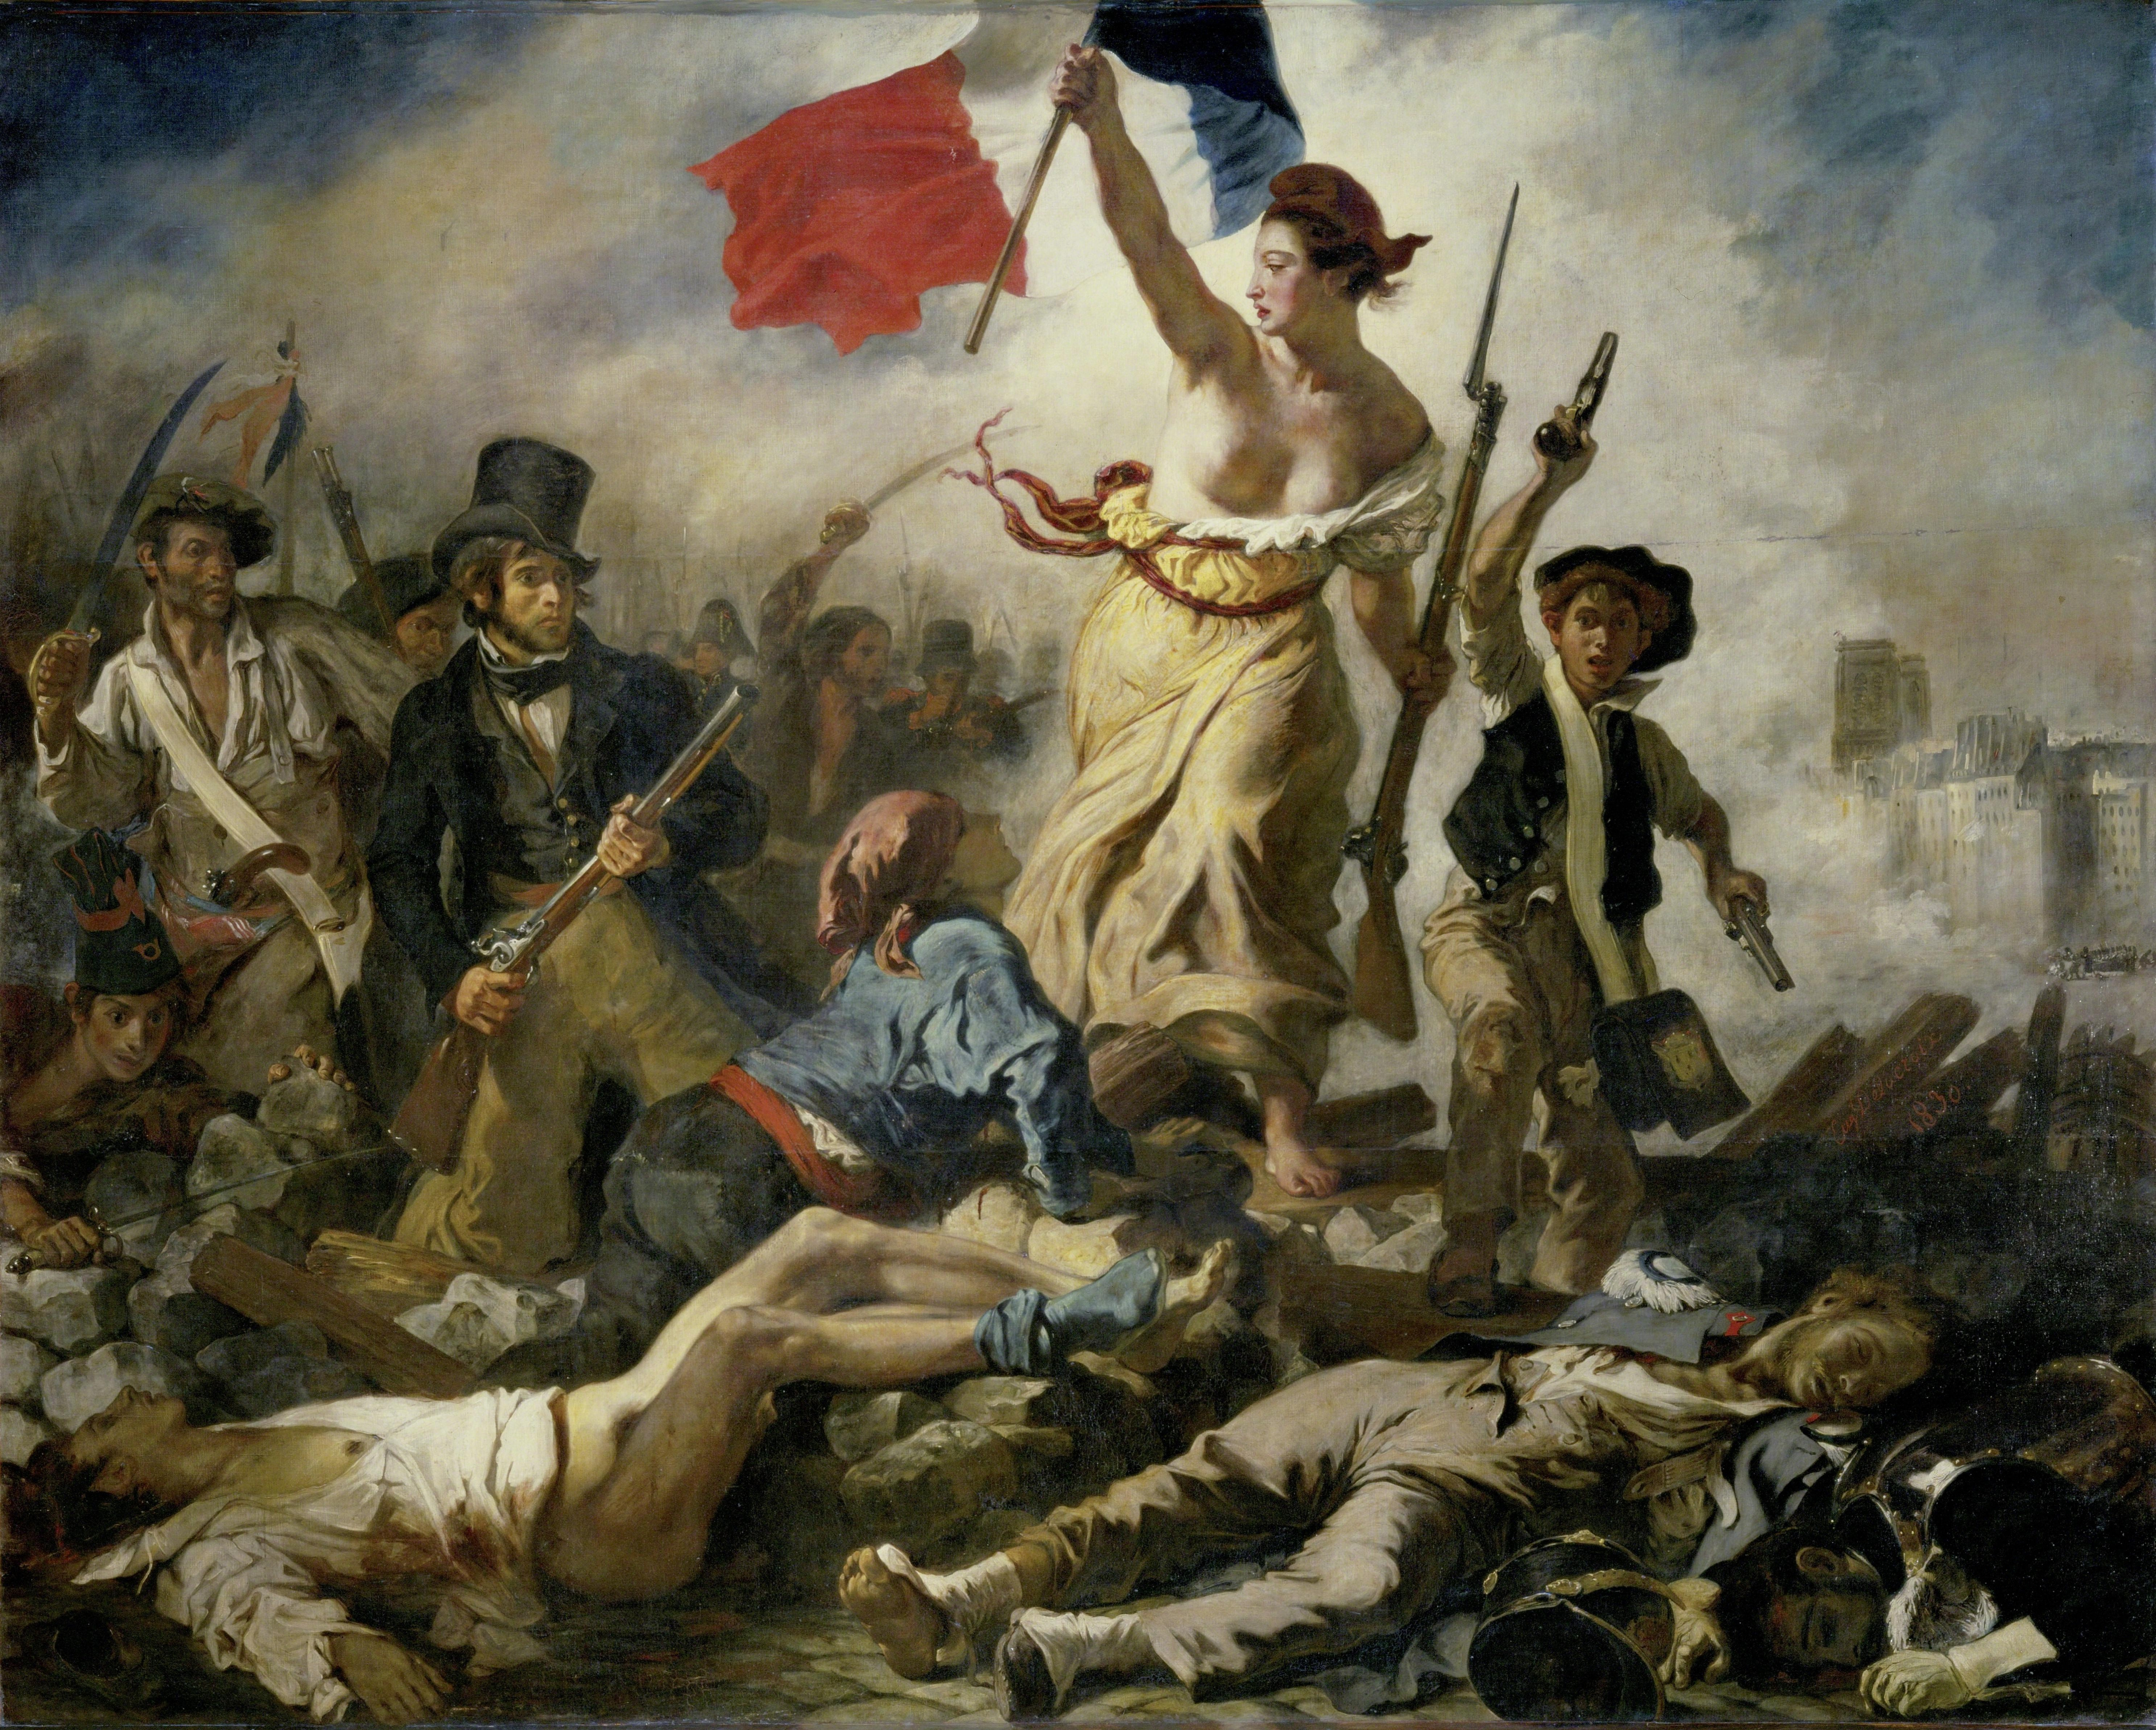
\includegraphics[width=4cm]{figura_15}
			\caption{\textit{A Liberdade guiando o povo}, de Eugène Delacroix.}
			\label{fig:mesh15}
		\end{figure}
		\par É interessante notar que a figura da Liberdade utiliza um barrete frígio, que representa a república (também a forma como a questão reformista aparecia nas artes plásticas).
		\par A ideia da Idade Média como Idade das Trevas fora uma expressão criada pelo Iluminismo. No Romantismo, há uma visão ambígua desse período. É interessante notar, nesse sentido, a forma como a arquitetura gótica era tida como sombria (relembre os gárgulas como forma de levar os fiéis à reflexão; além disso, com o tempo - sobretudo na Revolução Industrial -, as catedrais foram ficando velhas e escuras, remetendo à percepção que se tinha da cultura gótica que é, na realidade, o contrário disso; evolução tecnológica que possibilitava construções mais altas e finas, permitindo maior circulação de ar e luz). A princípio, é uma arquitetura da luz, mas cuja percepção se altera com o decorrer dos séculos (expoente na literatura com o \textit{Drácula}).
		\par A ideia da \textbf{libertinagem} também era muito presente. Trata-se de um estilo de vida amoral voltado para a satisfação dos prazeres, sem qualquer freio moral (inserido em uma sociedade cristã que valoriza a castidade, a temperança e a virgindade da mulher), em uma tentativa de corromper a família. É referida por alguns autores como \textit{dom juanismo}. Dom Juan é uma figura que já existia no imaginário europeu; seu objetivo é obter o maior prazer sexual possível, seduzindo mulheres virgens e casadas. Até então, suas histórias sempre possuíam um final ruim, em uma forma de apresentar uma punição. Com o Romantismo, no entanto, Lord Byron escreve um poema chamado \textit{Dom Juan}, no qual tenta heroificar a figura do libertino, que se torna quase como um anti-herói (a figura de Lord Byron se mistura com a de seus personagens).
		\par Retornando às temas das perversões sexuais, em temas como incesto, necrofilia e sadismo, é válido mencionar algumas de suas origens. O sadismo, por exemplo, possui origem literária com Marquês de Sade, que possui uma literatura pornográfica que explora a violência explícita. Estava preso no período da queda da Bastilha, mas após ser solto, é preso novamente pelo governo revolucionário. O masoquismo, por sua vez, tem origem em Sacher-Masoch e sua literatura gótica, que fugiam do aceitável pelos padrões vitorianos.
		\par Também é igualmente importante diferenciar o erotismo, que provoca a imaginação, sugere, e a pornografia, com o intuito de diretamente excitar sexualmente.
		\par Na ideia do direito natural, a natureza estaria fundada em certas leis naturais. Marquês de Sade, por exemplo, possui uma visão da natureza como mal cósmico, pois o ser humano deve viver de acordo com as leis impostas impostas por esta, que são destrutivas.
		\par Por fim, evidenciamos a heroificação dos criminosos, como indivíduos que se rebelam contra as imposições sociais (identificação dos interesses do público em assassinatos descritos em jornais). Narrativas de assassinatos pela perspectiva do assassino, estuprador, sequestrador, etc.
		
		\chapter{Romantismo em Portugal}
		\par Alexandre Herculano fora o introdutor do romance histórico, medievalista, em Portugal. \textit{Eurico, o presbítero}, é uma de suas obras mais notáveis.
		\par Camilo Castelo Branco, por sua vez, popularizara o folhetim (de criação francesa), e também escrevera diversas novelas passionais, narrativas em prosa de média extensão que tratam principalmente de relações amorosas\footnote{Algo que cabe ser mencionado é a etimologia do termo paixão. Derivado do latim \textit{passio}, significava, a princípio, sofrimento, o ato de suportar alguma emoção, em geral, negativa. Nesse sentido, é interessante notar a relação entre o termo e a obra \textit{Amor de perdição}.}. É autor de \textit{Amor de perdição}, a sua obra mais famosa.
		\par Por fim, temos Almeida Garrett, o principal poeta do Romantismo em Portugal, e autor de \textit{Viagem na minha terra}, um romance digressivo.
		
		\chapter{Romantismo no Brasil}
		\par O século XIX foi um período de grandes mudanças dentro do território brasileiro, e a situação do país no contexto geopolítico internacional mudara consideravelmente. Em 1822 ocorrera a independência do Brasil em relação a Portugal, tornando assim a região uma nação independente. Após um período marcado por turbulências políticas e um breve momento de regência, iniciaria-se o Segundo Reinado, com o monarca Dom Pedro II, que perduraria por quase meio século. O Romantismo chega ao país justamente nesse período, e teve papel fundamental no processo de construção de uma \textbf{identidade nacional brasileira}. A revista \textit{Nitheroy}, publicada pela primeira vez em 1836 por estudantes brasileiros em Paris, na França, é considerada a primeira publicação do Romantismo brasileiro. De autoria de Gonçalves Magalhães, \textit{Suspiros poéticos e saudades}, por sua vez, é o primeiro livro de poesias do Romantismo no país. Nota-se, no entanto, que as primeiras obras desse estilo de época ainda possuíam diversos elementos árcades, neoclássicos, identificados no contexto de um \textit{Romantismo de transição} (na própria revista citada anteriormente encontramos muitas dessas características).
		\par Em um primeiro momento, o Romantismo esteve intimamente relacionado com os projetos políticos do Segundo Reinado. Estava inserido em um período anterior de grandes turbulências, instabilidades políticas que seguiram da regência, com inúmeros indivíduos contrários com a forma pela qual a independência fora conquistada. Em relação a esse processo, a própria figura de Dom Pedro I também atuara como elemento de instabilidade, em paralelo com a situação da União Ibérica, à medida em que o rei de Portugal não poderia assumir essa mesma posição em outro reino, em nosso caso, o Brasil. Todo esse cenário de confusão política culminaria, em 1840, na execução do Golpe da Maioridade, marco inicial para o Segundo Reinado.
		\par Assumindo o trono pouco tempo antes de completar 15 anos, diversos eram os problemas a serem enfrentados pelo monarca. Em especial, Dom Pedro II desejava a criação de um sentimento de pertencimento ao Brasil, a adoção de uma identidade nacional, em especial com o intuito de acabar com as revoltas que assolaram o território anos antes. Para tanto, elaborara um projeto político de construção de uma identidade nacional como instrumento ideológico de manutenção da integridade territorial brasileira. Uma das principais formas de fomento a essa identidade fora a criação de uma cultura autônoma em relação à europeia e, em especial, portuguesa. É interessante notar, nesse sentido, o teor da frase ``Eu nasci e cresci no Brasil''; o processo é tratado quase como um acidente geográfico, em oposição com a frase ``Eu sou brasileiro''. Veja a forma como esse sentimento de identidade é fabricado, fruto de decisões políticas dentro de determinado contexto. Lembre-se, também, do processo de construção do samba como um ritmo nacional, que ainda que possuísse origens no Rio de Janeiro, a capital do país na época, era um gênero musical tão regional quanto o forró. Ao longo do regime militar a questão da identidade nacional também se fez fortemente presente.
		\par A fim de melhor compreender os primórdios do Romantismo no Brasil, outras características da sociedade brasileira merecem maior atenção. Em primeira análise, lembre-se de que uma taxa inferior a 10\% da população brasileira era alfabetizada. Dessa forma, o processo de construção de uma identidade nacional por meio da literatura concernia apenas a elite brasileira, a classe social que possuía recursos, influência regional, capacidade de mobilização da sociedade e, sobretudo, controle político dos outros níveis de poder (não era necessário desenvolver tal sentimento entre as classes menos favorecidas, que não detinham poder econômico e tampouco político) — o processo ocorrera de cima para baixo. Na visão de Dom Pedro II, era necessário subordinar a elite ao poder do Estado e, para tanto, era necessária uma identidade a esses indivíduos, para que todos os que nascessem no país se sentissem parte deste.
		\par Além disso, cabe mencionar a importância da literatura como difusora da identidade nacional e de conhecimentos sobre o Brasil — tratada tanto como fonte de entretenimento como meio de transmissão de determinado conhecimento ou ideia, especialmente em uma sociedade, na maior parte, analfabeta. Com efeito, nesse período, o ambiente intelectual europeu possuía uma considerável especialização: o meio acadêmico havia criado a figura dos especialistas (médicos, biólogos, matemáticos, etc.). No Brasil, em contrapartida, o acadêmico possuía uma vida incipiente e muito precária. Nesse contexto, durante o período colonial, era comum que os jovens da elite estudassem em Coimbra, Portugal (frequentemente, cursavam Direito), para então retornar ao país, uma vez que ainda não existiam instituições de ensino superior no Brasil (criadas posteriormente por Dom Pedro I, por meio do curso de Direito de Recife, em Pernambuco, assim como o curso de Direito do Largo de São Francisco - integrado à Universidade de São Paulo (USP) anos depois). Por essa razão, o intelectual brasileiro era, de maneira geral, um homem de letras, com uma formação humanística e mais genérica, de baixa especialização; o leitor brasileiro do século XIX não era um consumidor de monografias históricas, por exemplo, mas de produções mais gerais, menos especializadas. Por conseguinte, a identidade nacional não fora construída por textos históricos ou antropológicos, mas por meio da literatura e, em especial, de narrativas de amor, permeadas por elementos da ficção (tanto na prosa quanto na poesia), contextualizadas em determinada localidade do Brasil. A educação também teve importante papel nesse processo, e a disciplina de História, por exemplo, fora acrescida ao currículo das universidades como forma de divulgação da história nacional (que interessava ao Estado) e, em análise mais geral, de fomento à identidade brasileira. \textbf{No Brasil, os esforços se concentraram na literatura, e não nas escolas ou outros meios acadêmicos}. É interessante traçar um paralelo com a Europa, na qual a literatura também fora utilizada como forma de criação de uma identidade nacional, mas para um público reduzido.
		\par Alguns acontecimentos também merecem ser citados. Primeiramente, elencamos a criação do Instituto Histórico Geográfico Brasileiro (IHGB) em outubro de 1838, o qual reunia o grupo dos homens de letras citados anteriormente. Ademais, é válido mencionar o financiamento pessoal de Dom Pedro II para a elaboração, por parte de Gonçalves Magalhães, da epopeia \textit{A Confederação dos Tamoios}, em 1856. Posteriormente, José de Alencar ainda escreveria uma nota de crítica sobre a obra, que seria rebatida pelo monarca, oculto por um pseudônimo.
		\par Como elemento principal das produções literárias desse período, figura o questionamento \textbf{Como é viver no Brasil?}, à medida em que se buscava a criação de um mosaico da cultura brasileira.
		\par Com o panorama histórico completo, iniciaremos o estudo da poesia romântica no Brasil, tradicionalmente dividida em três gerações: Indianismo, Ultrarromantismo e Condoreirismo.
			\section{Indianismo}
			\par A primeira geração do Romantismo no Brasil fora fortemente marcada pelo nacionalismo. Na Europa, sua principal manifestação se deu por meio do medievalismo, a idealização da Idade Média; no Brasil o processo é, naturalmente, impossível. Caracterizado pela exaltação e idealização da natureza brasileira (noção de \textbf{país novo}, caracterizado pela abundância de recursos naturais como promessa de um futuro grandioso). O índio como símbolo da nacionalidade e figura síntese das virtudes nacionais. Desenvolvimento de um país: colonização por povoamento ou exploração, independentemente se essa ocorrera ou não tardiamente. Revolução Industrial, em contraponto com o valor dos recursos naturais do Brasil (esta muda a lógica capitalista, de forma que o Brasil se encontra preso no capitalismo mercantil, do sistema colonial). Manifesta-se por meio da exaltação da natureza brasileira, sempre relacionada à noção de \textbf{país novo} (riqueza natural como promessa de uma futura grandeza nacional), tratada como característica que diferenciava o Brasil dos países europeus, que já sentiam os efeitos ambientais decorrentes da Revolução Industrial. Nesse sentido, o Brasil, apesar de ser um país muito novo, possui muitas riquezas naturais, de forma que um dia o país será uma grande potência. Todavia, note como a idade em pouco ou nada influencia (como o exemplo dos Estados Unidos e da Austrália), e a riqueza natural pode, muitas vezes, significar dependência econômica, em especial na lógica do capitalismo industrial. Idealização da figura do índio, símbolo da nacionalidade brasileira (relembre que o homem branco era descendente dos europeus; neste momento, o objetivo era o distanciamento destes; por outro lado, haviam também os negros, mas que eram relacionados à escravidão; restara o índio). O programa de extermínio indígena levado a cabo pela Coroa Portuguesa havia sido bem sucedido, de forma que o contato com indígenas era incomum no cotidiano da população (indianismo de gabinete). As fontes utilizadas pelos escritores era, além de sua própria imaginação, a literatura de viajantes, relatos de viagens desenvolvidos ao longo do período colonial, principalmente por jesuítas, e destinadas sobretudo ao público europeu. Tal processo fora iniciado com a carta de Pero Vaz de Caminha. O grande problema de se basear em tais textos se deve ao fato que possuem uma visão pautada eurocêntrica. Na própria carta do descobrimento, por exemplo, lembre-se de que a primeira providência tomada pelos portuguesas fora a celebração de uma missa. O erro está em acreditar, por exemplo, que necessariamente uma religião se baseia em símbolos externos. Os nativos perceberam o rito dos portugueses, mas estes não o fizeram (literatura etnocêntrica). Outra fonte da qual os escritores indianistas utilizavam era o indianismo romântico francês (François-René de Chateaubriand), que utilizara do índio como uma representação do mito do bom selvagem (lembre-se de Rousseau, ``o homem nasce puro, inocente, mas a sociedade o corrompe''). O índio é visto como uma síntese das virtudes nacionais, i.e., todas as qualidades que se deseja atribuir ao povo brasileiro são projetadas na figura do índio. Este, ao mesmo tempo em que é corajoso, também é generoso, altruísta (adaptação da figura do cavaleiro medieval da literatura romântica europeia). O brasil não teve uma Idade Média. O período correspondente seria a colonização, em que o cavaleiro é substituído pela figura do índio (idealizado, sem precisão antropológica e etnográfica).
				\subsection{Gonçalves Dias}
				\par Expoente da primeira geração romântica no Brasil (não confundir com Gonçalves Magalhães, autor do primeiro livro de poesias), era um mulato que estudou em Portugal. Assim como outros poetas desta geração (Álvares de Azevedo e Castro Alves), contraíra tuberculose, ainda que não tivesse morrido diretamente pelos efeitos da doença (veio a óbito em um naufrágio).
					\subsubsection{I-Juca-Pirama}
					\par Narra a história de um índio de mesmo nome, filho de um cacique cuja tribo está em conflito com outra, os aimorés - praticavam atos de antropofagia, com o intuito de, entre outros fatores, absorver a força do inimigo. Em dado momento da história, I-Juca-Pirama é capturado e, no momento de sua morte, chora e implora pelo perdão de seus inimigos. Por essa razão, os aimorés desistem de matar e se alimentar do jovem, à medida em que não desejam ingerir a carne de um índio fraco que temeu a morte. Ao retornar à tribo, descreve os acontecimentos para seu pai, o cacique, que o expulsa da tribo alegando não ser digno. Posteriormente, e outro conflito entre os tupis e os aimorés, I-Juca-Pirama aparece e liberta a sua tribo, mas acaba morrendo no processo (redenção em batalha). Destacamos o processo de nacionalização da ética guerreira, que o Romantismo europeu explorara por meio da figura do cavaleiro medieval. Um das partes mais importantes da obra é o Canto IV, reproduzido abaixo; escrito em redondilha menor (cinco sílabas poéticas, com icto - tônica obrigatória em determinada sílaba - na segunda e quinta sílabas poéticas), possui um ritmo marcante, utilizando-se de um canto de morte como um canto de batalha (como observado pelo emprego de \textit{guerreiros} como vocativo). Trata dos cruéis conflitos disputados pelas tribos, o cansaço proveniente de tais acontecimentos, e lembra de momentos de quando ainda estava na terra no natal. 
					\poemtitle{Canto IV}
					\settowidth{\versewidth}{Guerreiros, ouvi:}
					\begin{verse}[\versewidth]
						Meu canto de morte, \\
						Guerreiros, ouvi: \\
						Sou filho das selvas, \\
						Nas selvas cresci; \\
						Guerreiros, descendo \\
						Da tribo Tupi.
						
						Da tribo pujante, \\
						Que agora anda errante \\
						Por fado inconstante, \\
						Guerreiros, nasci: \\
						Sou bravo, sou forte, \\
						Sou filho do Norte; \\
						Meu canto de morte, \\
						Guerreiros, ouvi.
						
						Já vi cruas brigas, \\
						De tribos imigas, \\
						E as duras fadigas \\
						Da guerra provei; \\
						Nas ondas mendaces \\
						Senti pelas faces \\
						Os silvos fugaces \\
						Dos ventos que amei.
						
						Andei longes terras, \\
						Lidei cruas guerras, \\
						Vaguei pelas serras \\
						Dos vis Aimorés; \\
						Vi lutas de bravos, \\
						Vi fortes — escravos! \\
						De estranhos ignavos \\
						Calcados aos pés.
						
						E os campos talados, \\
						E os arcos quebrados, \\
						E os piagas coitados \\
						Sem seus maracás; \\
						E os meigos cantores, \\
						Servindo a senhores, \\
						Que vinham traidores, \\
						Com mostras de paz.
						
						Aos golpes do imigo \\
						Meu último amigo, \\
						Sem lar, sem abrigo \\
						Caiu junto a mi! \\
						Com plácido rosto, \\
						Sereno e composto, \\
						O acerbo desgosto \\
						Comigo sofri.
						
						Meu pai a meu lado \\
						Já cego e quebrado, \\
						De penas ralado, \\
						Firmava-se em mi: \\
						Nós ambos, mesquinhos, \\
						Por ínvios caminhos, \\
						Cobertos d’espinhos \\
						Chegamos aqui!
						
						O velho no entanto \\
						Sofrendo já tanto \\
						De fome e quebranto, \\
						Só queria morrer! \\
						Não mais me contenho, \\
						Nas matas me embrenho, \\
						Das frechas que tenho \\
						Me quero valer.
						
						Então, forasteiro, \\
						Caí prisioneiro \\
						De um troço guerreiro \\
						Com que me encontrei: \\
						O cru dessossego \\
						Do pai fraco e cego, \\
						Enquanto não chego, \\
						Qual seja — dizei!
						
						Eu era o seu guia \\
						Na noite sombria, \\
						A só alegria \\
						Que Deus lhe deixou: \\
						Em mim se apoiava, \\
						Em mim se firmava, \\
						Em mim descansava, \\
						Que filho lhe sou.
						
						Ao velho coitado \\
						De penas ralado, \\
						Já cego e quebrado, \\
						Que resta? - Morrer. \\
						Enquanto descreve \\
						O giro tão breve \\
						Da vida que teve, \\
						Deixa-me viver!
						
						Não vil, não ignavo, \\
						Mas forte, mas bravo, \\
						Serei vosso escravo: \\
						Aqui virei ter. \\
						Guerreiros, não coro \\
						Do pranto que choro; \\
						Se a vida deploro, \\
						Também sei morrer.
					\end{verse}
				\par Por fim, citamos \textit{Canção do exílio}, potencialmente a obra mais famosa do autor. Novamente, há a exploração de temas que permeiam um sentimento de nacionalismo. 
				\poemtitle{Canção do exílio}
				\settowidth{\versewidth}{Onde canta o sabiá;}
				\begin{verse}[\versewidth]
					Minha terra tem palmeiras, \\
					Onde canta o sabiá; \\
					As aves, que aqui gorjeiam, \\
					Não gorjeiam como lá.
						
					Nosso céu tem mais estrelas, \\
					Nossas várzeas têm mais flores, \\
					Nossos bosques têm mais vida, \\
					Nossa vida mais amores.
					
					Em cismar, sozinho, à noite, \\
					Mais prazer eu encontro lá; \\
					Minha terra tem palmeiras, \\
					Onde canta o sabiá.
					
					Minha terra tem primores, \\
					Que tais não encontro eu cá; \\
					Em cismar - sozinho, à noite - \\
					Mais prazer eu encontro lá; \\
					Minha terra tem palmeiras, \\
					Onde canta o sabiá.
					
					Não permita Deus que eu morra, \\
					Sem que eu volte para lá; \\
					Sem que desfrute os primores \\
					Que não encontro por cá; \\
					Sem qu'inda aviste as palmeiras, \\
					Onde canta o sabiá.
					\end{verse}
			\section{Ultrarromantismo}
			\par A segunda geração romântica, frequentemente referida também como byronismo. Trata-se de um termo pejorativo utilizado na Europa em referência à vertente sentimentalista do Romantismo português. De maneira geral, fora caracterizada pelo sentimentalismo, subjetivismo (a poesia dedicada aos sentimentos e emoções do indivíduo), egotismo (o poeta romântico fala preferencialmente de si mesmo) e  evasionismo (o indivíduo em conflito com a realidade foge para a sua vida interior; fuga para o mundo interior ou para um passado idealizado, como a infância). Compreende, sobretudo, uma poesia que não possui caráter social, i.e. não tratará das principais pautas sociais e políticas de sua época.
			\par Outra característica muito presente nessa vertente é a idealização da figura feminina, citada no capítulo de introdução. Comumente era representada a cena da virgem adormecida e o poeta tímido. A mulher é tratada como um ser valorizado por sua pureza e castidade (em paralelo com a figura da mulher corrompida pela prostituição, por exemplo). A temática do \textit{medo do amor}, expressão utilizada por Mário de Andrade para se referir do niilismo do amor dessa segunda geração. A figura do adolescente tímido, mesmo que o eu lírico não se apresente como adolescente, este revela demasiada insegurança em relação às mulheres, e não sabe como se portar. Do latim \textit{timere}, aquele que tem medo, no caso, de não ser correspondido e por isso sofrer muito. Motivo (uma cena recorrente, que se repete) da virgem adormecida. Eram muito famosos os poemas nos quais o eu lírico apenas observa a amada enquanto dorme, sem se aproximar ou se declarar (satisfação do interesse erótico). O imaginário a partir da vida priva, reclusa das mulheres, em meio à valorização da pureza e virgindade femininas, e o prestígio romântico da mulher, sempre chamada de virgem, anjo (distanciamento da carnalidade), criança (ênfase na pureza e inocência), irmã (não um amor sexualizado, carnal ou satânico, mas um amor puro), etc. Lembre-se também da questão da melancolia e a relação estabelecida com o \textit{spleen}, bile negra — fluido produzido pelo baço.
			\par Também se faz presente o satanismo, comumente referido como byronismo, e a utilização de temas macabros (relacionados à morte), perversões sexuais e \textit{dom juanismo} (libertinagem). Lembre-se de que Lord Byron transformara a figura de Dom Juan em um herói. 
				\subsection{Casimiro de Abreu}
				\par Um dos principais autores dessa geração, também conhecido como o \textbf{poeta da infância}, uma vez que em muitos poemas, em um processo de idealização da vida infantil e, em última análise, do campo, retorna para sua casa de origem.
				\par \textit{Carece de mais informações.}
				\subsection{Álvares de Azevedo}
				\par Álvares de Azevedo, em paralelo com Gonçalves Dias, é o principal autor da segunda geração romântica (Ultrarromantismo); divide espaço com Casimiro de Abreu, o poeta da infância. Bernardo Guimarães (escritor de \textit{A escrava Isaura}), por sua vez, foi um dos maiores expoentes da corrente satanista e sentimentalista da segunda geração.
					\subsubsection{Noite na taverna}
					\par Exemplo notável da vertente satânica do Ultrarromantismo. Acompanhamos um grupo de libertinos (sem freios morais) que, após uma noite de orgia, se reúnem uma taverna, onde passam a noite contando histórias uns aos outros como forma de entretenimento. O primeiro conto, por exemplo, possui elementos relacionados diretamente com a necrofilia.
					\subsubsection{Lira dos vinte anos}
					\par É interessante notar a diferença existente entre a primeira e a segunda parte da obra. Na primeira parte estão todas as convenções da vertente sentimentalista do Romantismo (os clichês da literatura sentimentalista romântica, como a observação da amada dormindo — ou mesmo a virgem morta\footnote{Na vertente satanista, \textit{aquilo que não era necrofilia, torna-se} (lembre-se de \textit{Noite na taverna}).}, que não é corrompida pelo pecado —, a tristeza pela vida, etc.).
					\par A segunda parte, por sua vez, é caracterizada por um realismo satírico e pela ironia. As convenções da primeira parte reaparecem rebaixadas ao plano da vida ordinária. Os mesmos lugares-comuns e convenções da primeira parte reaparecem em uma perspectiva irônica, tomadas pelo realismo satírico (note que a abordagem anterior é marcada pelo evasionismo), trazendo-os para o cotidiano. Lembre-se do conceito de decoro: para cada tema, há um estilo e tom apropriado. Nesse sentido, o amor é abordado no estilo alto, na medida em que no estilo baixo se aborda a vida cotidiana, ordinária, e a vida do homem comum. Álvares de Azevedo toma os temas da poesia lírica e os transfere para a vida cotidiana, de forma a receber uma abordagem humorística (convenções rebaixadas ao plano da vida ordinária).
					\par Para entender esse processo, Marx descreve que a burguesia da qual o Romantismo é expressão é muito crítica consigo mesma, e está em conflito com o antigo regime. Constrói-se a ideia de uma burguesia anti-burguesa: esta imagina que a sociedade oprime o indivíduo, mas quem a controla é a própria burguesia, de forma que a burguesia oprime o próprio burguês. Há uma sátira a partir dos valores que a burguesia reflete na literatura, o fenômeno da literatura anti-burguesa (vertente reformista do Romantismo), cujo instrumento de crítica é a ironia. \textbf{A repetição se torna cansativa, e por isso se busca uma nova abordagem dos lugares-comuns}.
					\par Analisaremos com maior cuidado cada uma das partes.
					\poemtitle{No mar (Parte I)}
					\settowidth{\versewidth}{Do sonho nas melodias,}
					\begin{verse}[\versewidth]
						Era de noite — dormias, \\
						Do sonho nas melodias, \\
						Ao fresco da viração, \\
						Embalada na falua, \\
						Ao frio clarão da lua, \\
						Aos ais do meu coração!
						
						Ah! que véu de palidez \\
						Da langue face na tez! \\
						Como teus seios revoltos \\
						Te palpitavam sonhando! \\
						Como eu cismava beijando \\
						Teus negros cabelos soltos!
						
						Sonhavas? — eu não dormia; \\
						A minh'alma se embebia \\
						Em tua alma pensativa! \\
						E tremias, bela amante, \\
						A meus beijos, semelhante \\
						Às folhas da sensitivas!
						
						E que noite! que luar! \\
						E que ardentias no mar! \\
						E que perfumes no vento! \\
						Que vida que se bebia \\
						Na noite que parecia \\
						Suspirar de sentimento!
						
						Minha rola, ó minha flor, \\
						Ó madresilva de amor, \\
						Como eras saudosa então! \\
						Como pálica sorrias \\
						E no meu peito dormias \\
						Aos ais do meu coração!
						
						E que noite! que luar! \\
						Como a brisa a soluçar \\
						Se desmaiava de amor! \\
						Como toda evaporava \\
						Perfumes que respirava \\
						Nas laranjeiras em flor!
						
						Suspiravas? que suspiro! \\
						Ai que ainda me deliro \\
						Entrevendo a imagem tua \\
						Ao fresco da viração, \\
						Aos ais do meu coração, \\
						Embalada na falua!
						
						Como virgem que desmaia, \\
						Dormia a onda na praia! \\
						Tua alma de sonhos cheia \\
						Era tão pura, dormente, \\
						Como a vaga transparente \\
						Sobre seu leito de areia!
						
						Era de noite — dormias, \\
						Do sonho nas melodias, \\
						Ao fresco da viração; \\
						Embalada na falua, \\
						Ao frio clarão da lua, \\
						Aos ais do meu coração \\
					\end{verse}
					\par De maiores convenções, o eu lírico observa a mulher amada dormindo sob um leito de flores (ou a estampa do lençol), na luz de lâmpadas. A amada é como se fosse a lua embalsamada (envolta) pela noite (referência ao processo de embalsamento, proporcionando um aspecto mórbido, que acrescenta sensualidade ao poema), em valorização de uma poesia mais doentia. Comparação da virgem adormecida com a virgem surgida no mar (relembre o nascimento da virgem Afrodite). Comparação com um anjo em meio as nuvens (prestígio romântico da mulher, de forma a torná-la mais espiritualizada). Velar um cadáver, com a utilizar de velas (os velórios atravessavam a noite). A maior prova de amor que o eu lírico oferece é morrer pela amada. Utilização do clichê da virgem adormecida, da qual o eu lírico não se aproxima.
					\poemtitle{É ela! É ela! (Parte II)}
					\settowidth{\versewidth}{E o eco ao longe murmurou — é ela!...}
					\begin{verse}
						É ela! é ela! — murmurei tremendo, \\
						E o eco ao longe murmurou — é ela!... \\
						Eu a vi... minha fada aérea e pura, \\
						A minha lavadeira na janela!
						
						Dessas águas-furtadas onde eu moro \\
						Eu a vejo estendendo no telhado \\
						Os vestidos de chita, as saias brancas... \\
						Eu a vejo e suspiro enamorado!
						
						Esta noite eu ousei mais atrevido \\
						Nas telhas que estalavam nos meus passos \\
						Ir espiar seu venturoso sono, \\
						Vê-la mais bela de Morfeu nos braços!
						
						Como dormia! que profundo sono!... \\
						Tinha na mão o ferro do engomado... \\
						Como roncava maviosa e pura! \\
						Quase caí na rua desmaiado!
						
						Afastei a janela, entrei medroso: \\
						Palpitava-lhe o seio adormecido... \\
						Fui beijá-la... roubei do seio dela \\
						Um bilhete que estava ali metido...
						
						Oh! De certo ... (pensei) é doce página \\
						Onde a alma derramou gentis amores!... \\
						São versos dela... que amanhã decerto \\
						Ela me enviará cheios de flores...
						
						Trem de febre! Venturosa folha! \\
						Quem pousasse contigo neste seio! \\
						Como Otelo beijando a sua esposa, \\
						Eu beijei-a a tremer de devaneio...
						
						É ela! é ela! — repeti tremendo, \\
						Mas cantou nesse instante uma coruja... \\
						Abri cioso a página secreta... \\
						Oh! meu Deus! era um rol de roupa suja!
						
						Mas se Werther morreu por ver Carlota \\
						Dando pão com manteiga às criancinhas, \\
						Se achou-a assim mais bela... eu mais te adoro \\
						Sonhando-te a lavar as camisinhas!
						
						É ela! é ela! meu amor, minh’alma, \\
						A Laura, a Beatriz que o céu revela... \\
						É ela! é ela! — murmurei tremendo, \\
						E o eco ao longe suspirou — é ela!
					\end{verse}
					\par Do realismo satírico, aborda o mesmo tema da cena da virgem adormecida, mas com algumas notórias diferenças. A utilização de fada aérea e pura nos remete ao plano da mulher idealizada, mas ao identificá-la como lavadeira, o autor traz o tema para a realidade cotidiana, com uma mulher pertencente às classes menos abastadas. O eu lírico mora no último andar da residência. Chita é um tecido barato. Morfeu é o deus dos sonhos. O eu lírico invade o quarto da amada no meio da noite para observá-la. Maviosa como sinônimo de delicada, ironia com a situação da amada roncando, que dormiu em meio ao trabalho. Quando o eu lírico se aproxima para beijá-la, encontra um bilhete. Pensando que se tratava de um poema para sua pessoa, o pega. Processo de inversão, na medida em que é o eu lírico quem espera as flores por parte da amada. O bilhete era, na verdade, uma lista de roupas dos clientes. Referência com a obra \textit{O sofrimento do jovem Werther}, que se apaixonara por Carlota enquanto a jovem distribuía pão para as crianças da casa. Camisinha como a vestimenta que permanecia por baixo das roupas. Referências à Beatriz de Dante Alighieri, e Laura de Petrarca.
					\par \textbf{A palavra de ordem do Romantismo é a idealização}.
			\section{Condoreirismo}
			\par A terceira geração do Romantismo no Brasil, caracterizada, sobretudo, pelo reformismo. Trata-se de uma das manifestações do conflito eu e o mundo, no qual o indivíduo percebe que o mundo não corresponde aos seus ideias. Assim, ao invés de se refugiar em seu interior ou mesmo nas lembranças de um passado idealizado, como ocorrera com os sentimentalistas, busca transformar a realidade. Ideia da literatura como um instrumento de transformação das consciências, em um projeto de mudança social (a literatura, por si ó, não é capaz de transformar a realidade, mas sim despertar a consciência dos indivíduos, estes sim aptos para tal). Dois dos valores fundamentais para essa vertente são o liberalismo e o combate à tirania, para o qual a liberdade pressupõe ganho social. O ser humano alcança a sua dignidade com o exercício da liberdade (econômica e política). Nesse sentido, é interessante citar a análise de Marx para o qual a burguesia das revoluções, a qual abandona se caráter revolucionário com o massacre do proletariado nas ruas de Paris (data definida pelo próprio autor). Em alguns países, o combate à tirania se descreve da deposição do antigo regime, em outros, no combate contra a Igreja (combate à tirania, a depender da conjuntura política).
			\par Condoreirismo deriva de condor, uma ave de grande envergadura (maior do hemisfério sul), a qual habita a Cordilheira dos Andes. Símbolo para o \textit{americanismo} (diferenciação dos países para com aqueles que o colonizaram), e metáfora para a figura do \textit{gênio}, o indivíduo que é naturalmente dotado de inteligência, sensibilidade e imaginação superiores a dos indivíduos comuns. Este, ao ser capaz de ver além, é capaz de guiar a humanidade para o caminho correto (farol para o caminho do progresso). Em paralelo, o condor voa alto, referência ao pensar além do que as pessoas são capazes (natureza diferente).
			\par De maneira geral, o maior compromisso com as causas políticas da época, e que mobilizara os liberais no século XIX, era o abolicionismo, discutido desde a década de 1820 (o republicanismo não era um consenso), assim como o compromisso com a democracia. O brasil, independentemente do sistema político, sempre fora um país pouco democrático (limitação dos direitos políticos, como o voto censitário). A participação feminina (acesso ao voto e ao trabalho) nunca foi uma pauta amplamente defendida pelos liberais. Ainda assim, o feminismo é um movimento que surgiu em meio ao liberalismo e, posteriormente, assumiu outros caminhos.
				\subsection{Castro Alves}
				\par Conhecido como o poeta dos escravos, foi o expoente da terceira geração. Mulato, morreu ainda jovem com um tiro no pé. Identificamos, em sua obra, um processo de erotização mais explícita, e a superação da ideia do jovem tímido.
				\poemtitle{O Povo ao poder}
				\settowidth{\versewidth}{Do Povo a sublime voz… }
				\begin{verse}[\versewidth]
					Quando nas praças se eleva \\
					Do Povo a sublime voz… \\
					Um raio ilumina a treva \\
					O Cristo assombra o algoz…
					
					Que o gigante da calçada \\
					De pé sobre a barrica \\
					Desgrenhado, enorme, nu \\
					Em Roma é catão ou Mário, 
					
					É Jesus sobre o Calvário, \\
					É Garibaldi ou Kosshut.
					
					A praça! A praça é do povo \\
					Como o céu é do condor\\
					É o antro onde a liberdade \\
					Cria águias em seu calor! 
					
					Senhor!… pois quereis a praça? \\
					Desgraçada a populaça \\
					Só tem a rua seu… \\
					Ninguém vos rouba os castelos
					
					Tendes palácios tão belos… \\
					Deixai a terra ao Anteu.
					
					Na tortura, na fogueira… \\
					Nas tocas da inquisição \\
					Chiava o ferro na carne \\
					Porém gritava a aflição. \\
					Pois bem … nesta hora poluta 
					
					Nós bebemos a cicuta \\
					Sufocados no estertor; \\
					Deixai-nos soltar um grito\\
					Que topando no infinito 
					
					Talvez desperte o Senhor. 
					
					A palavra! Vós roubais-la \\
					Aos lábios da multidão \\
					Dizeis, senhores, à lava \\
					Que não rompa do vulcão.\\
					Mas qu’infâmia! Ai, velha Roma, \\
					Ai cidade de Vendoma, \\
					Ai mundos de cem heróis,\\
					Dizei, cidades de pedra,\\
					Onde a liberdade medra\\
					Do porvir aos arrebóis.
					
					Dizei, quando a voz dos Gracos \\
					Tapou a destra da lei? \\
					Onde a toga tribunícia \\
					Foi calcada aos pés do rei? \\
					Fala, soberba Inglaterra, \\
					Do sul ao teu pobre irmão; \\
					Dos teus tribunos que é feito? \\
					Tu guarda-os no largo peito \\
					Não no lodo da prisão. \\
					No entanto em sombras tremendas\\
					Descansa extinta a nação \\
					Fria e treda como o morto. \\
					E vós, que sentis-lhes os pulso \\
					Apenas tremer convulso \\
					Nas extremas contorções… \\
					Não deixais que o filho louco \\
					Grite “oh! Mãe, descansa um pouco \\
					Sobre os nossos corações”. 
						
					Mas embalde… Que o direito \\
					Não é pasto de punhal. \\
					Nem a patas de cavalos \\
					Se faz um crime legal… \\
					Ah! Não há muitos setembros, \\
					Da plebe doem os membros \\
					No chicote do poder, \\
					E o momento é malfadado \\ 
					Quando o povo ensanguentado \\
					Diz: já não posso sofrer.
					
					Pois bem! Nós que caminhamos \\
					Do futuro para a luz, \\
					Nós que o Calvário escalamos \\
					Levando nos ombros a cruz, \\
					Que do presente no escuro \\
					Só temos fé no futuro, \\
					Como alvorada do bem, \\
					Como Laocoonte esmagado \\
					Morreremos coroado \\
					Erguendo os olhos além. 
					
					Irmãos da terra da América, \\
					Filhos do solo da cruz, \\
					Erguei as frontes altivas, \\
					Bebei torrentes de luz..\\
					Ai! Soberba populaça, \\
					Dos nossos velhos Catões, \\
					Lançai um protesto, ó povo, \\
					Protesto que o mundo novo \\
					Manda aos tronos e às nações.
				\end{verse}
				\par A praça simboliza a \textit{ágora}, a qual, por sua vez, simboliza o local onde todas as classes sociais se encontram (metonímia para o espaço público). A imagem de raio está relacionada ao sentido iluminista de razão, afastada da ignorância. Algoz como carrasco, tirano, e o povo como Cristo. Barrica como barricada, um obstáculo desenvolvido de maneira improvisada, e muito relacionado com as revoltas populares (Paris e a designação de \textit{cidade das barricadas}). Gigante pois o povo representa a maioria da população. Desgrenhado, enorme e nu pois o povo é pobre, e tem o direito de se revoltar contra a tirania. Os heróis da república romana. Garibaldi foi um dos heróis da unificação italiana, e Kosshut um líder popular indiano (cada um em seus contextos representam a luta contra a tirania). O espaço público deve ser dominado pelo povo. Gênio é aquele que possui a capacidade de falar em nome do povo (meidação pelo poeta). Antro é um local fechado, na qual o calor da razão gerará águias (pensamento autônomo, com a liberdade de voar conforme a vontade). O senhor representa os detentores do poder econômico, os quais possuem tudo, e também desejam se apoderar da praça, o espaço público (também querer o poder político). Anteu é um gigante que, enquanto em contato com a Terra, é indestrutível. Representa o povo, o qual, enquanto estiver no domínio da praça, jamais será vencido (na democracia, torna-se uma força imperiosa, incapaz de ser barrada). Defesa da ideia de democracia e separação dos interesses econômicos e privados dos interesses públicos.
				\poemtitle{O navio negreiro}
				\settowidth{\versewidth}{Algo aqui.}
				\begin{verse}[\versewidth]
					Algo aqui.
				\end{verse}
				\par É interessante notar a relação estabelecida entre o eu lírico e Deus. Mostra-se horrorizado com o tráfico de escravos. Referência aos elementos da natureza, e questionamentos: por que as ondas do mar permitem que esta mancha na história humana aconteça? Há um pedido para que estes impeçam o tráfico.
				\par Contexto da \textit{Lei para inglês ver}, Eusébio de Queirós.
				\par Os desgraçados são os indivíduos sequestrados na África e lavados na condição de escravos para outras localidades. Algoz são os responsáveis por esse tráfico.
				\par Ideia de que Deus e a natureza não se importam com os escravizados, e são cúmplices desse crime. Libérrima como superlativo de livre, e significa liberdade (aquela que inspira os versos do eu lírico).
				\par A terra é a esposa, casada com a luz, local de onde vieram (na visão de Castro Alves, a África é um local muito iluminado — imagem estereotipada do deserto e do continente africano).
				\par Os tigres manchados, com listra, foram reduzidos à condição de míseros escravos, sem ar e sem luz (referência aos porões dos navios negreiros). Sem razão em uma concepção liberal, para a qual o indivíduo se torna plenamente humano com o exercício da liberdade (na qual se inclui a liberdade de pensar e a razão).
				\par Agar era a escrava de Abraão, a qual deu a luz à Ismael. Ismaelitas como muçulmanos. compromisso com as causas políticas de sua época, sobretudo com a abolição da escravidão. Poesia reformista, na qual o poeta é a representação do gênio (condor).
		\par A prosa romântica no Brasil, por sua vez, seguiu um caminho em muitos aspectos semelhante. Lembre-se de que no século XIX não havia internet, cinema, televisão ou rádio, e a principal forma de entretenimento das classes letradas no ambiente doméstico se dava por meio da literatura e, em especial, dos folhetins. Esses impressos surgiram na França e rapidamente alcançaram grande popularidade: eram baratos e de fácil leitura, além de possuírem uma estrutura narrativa com ganchos e reviravoltas de forte apelo popular. No Brasil o processo não seria diferente, ainda com a especificidade de uma minoria alfabetizada, concentrada nas grandes cidades do país (no Rio de Janeiro, por exemplo, a população chegava ao dobro da média nacional).
		\par Nesse período, tornou-se comum o consumo de folhetins populares (o próprio escritor José de Alencar lia folhetins semanalmente para a família, e outros indivíduos não necessariamente alfabetizados). Uma dessas obras mais famosas foi \textit{O guarani}, também de José de Alencar. Pelas cidades comumente haviam grupos que se reuniam semanalmente para a leitura de folhetins, sob a luz dos postes.
		\par Nesse contexto, como se tratava se uma prosa feita para ser lida em voz alta, não cabia uma linguagem demasiadamente coloquial ou oralizada, mas mais simples para caber na boca das pessoas. É interessante como os próprios autores os escreviam tendo em vista que seriam lidos em voz alta.
		\par Camilo Castelo Branco foi um dos primeiros autores de folhetins do país. Já o primeiro folhetim a fazer grande sucesso, e que serviu de inspiração para outros autores, foi \textit{A moreninha}, de Joaquim Macedo (posteriormente reunido em livros). Também é válido mencionar o papel de José de Alencar no processo de construção de um português brasileiro, enfatizando em sua linguagem diferentes colocações pronominais (ênclise, próclise e mesóclise), por exemplo, em uma tentativa de elaborar uma literatura nacionalista.
		\par De maneira geral, no século XIX, o termo \textit{romance} se referia, sobretudo, às novelas. Isso pois, como instrumento de investigação da realidade nacional, haviam três principais formas do gênero narrativo utilizadas: o conto (não adequado para o folhetim, dada a duração), a novela (a melhor forma narrativa para o folhetim semanal, com uma narrativa de média extensão) e o romance (não convinha, pois os romances do século XIX, frequentemente, eram muitos grandes — \textit{Guerra e paz}, por exemplo), as quais também variavam em número de tramas, complexidade do enredo, etc. Curiosamente, na língua inglesa, ocorrera o processo contrário, com os termos \textit{novel} e \textit{romance}.
		\par Em síntese: os escritores brasileiros tiveram um papel fundamental, por meio da literatura, na construção de uma identidade nacional. Em especial, o Brasil carecia do intelectual especializado (paralelamente, na Europa já havia a figura do matemático, filósofo, etc.) e, consequente, não haviam indivíduos aptos a escrever ou mesmo ler textos acadêmicos, e sim literatura, desenvolvida por esses homens de letras. De maneira geral, as produções eram mais simples e, por conseguinte, mais fáceis para transmitir à população a imagem e sentimento de pertencimento. Os livros circulavam, e a literatura, enquanto entretida, também transmitia um conjunto de valores (dentro da literatura, a principal forma que vai sintetizar isso é o romance).
		\par ao invés de escrever um texto monográfico sobre o período do colonialismo, por exemplo, narra-se um romance contextualizado nesse período. O romance será utilizado para descrever as diferentes regiões do Brasil, como elo entre os indivíduos do Rio de Janeiro e de outras localidades, seja do Norte ou Sul do Brasil. A linguagem da poesia é mais estilizada, com rimas e um vocabulário mais estilizado, sintetizadas em uma métrica e com inúmeras referências culturais, que requererem um leitor mais especializado. O romance, por outro lado, narra uma história de amor com muitas páginas, possibilitando a explicação de referências (leitura facilitada que se abria a um público maior).
		\par José de Alencar tinha um projeto de escrever um romance para cada região do Brasil, com o objetivo de criar um grande panorama da realidade social e política do Brasil (inspiração em Balzac, escritor da \textit{Comédia humana}, que descrevia a sociedades francesas do século XIX).
		\par Algo importante merece ser mencionado: \textbf{a sociedade brasileira não era tão complexa quanto a francesa (urbanizada e industrializada)}. Por essa razão, (?).
			\section{José de Alencar}
			\par José de Alencar é o autor mais importante da prosa romântica no Brasil, e escrevera em todas as vertentes do Romantismo no país. Um dos valores burgueses que inspirou o Romantismo foi o nacionalismo, cuja principal manifestação foi o romance histórico (desenvolvido pelo escocês Arthur Scott). No Romantismo europeu, o supracitado romance possuía características medievalistas, com o cavaleiro atuando como protagonista.
			\par O Brasil não passou pela Idade Média (derivada do colonizador) por uma razão cronológica. Dessa forma, quando o romance histórico, de caráter nacionalista, chegou ao país, transformou-se em um romance indianista (adaptação do romance histórico para o contexto histórico brasileiro). Os romances indianistas se passavam, via de regra, no primeiro século de colonização portuguesa (adaptação da Idade Média para o país).
			\par Tudo o que os escritores sabiam acerca dos indígenas se baseava nos escritos de viajantes dos séculos anteriores (alguns dos personagens de \textit{Iracema} de fato existiram). Esse olhar sobre a cultura indígena possuía um viés etnocêntrico. \textit{Viagens maravilhosas}, um gênero literário presente, por exemplo, nas obras de Marco Polo, mesclando os relatos fantasiosos de viagem com os relatos verídicos no imaginário europeu. José de Alencar chegou a citar que já não existiam indígenas no Brasil (descolamento da realidade; indianismo de gabinete/escritório).
			\par Em ordem cronológica, as três principais obras de José de Alencar são \textit{O guarani}, \textit{Iracema} e \textit{Ubirajara}. A figura do indígena cumpre a mesma função do cavaleiro na literatura romântica: síntese das virtudes nacionais (valores como bravura, generosidade, altruísmo, herdados pelos brasileiros por meio do sangue — atavismo).
				\subsection{O guarani}
				\par Narra a história do índio Peri, que se apaixona pela filha de um colonizador português (personalidade histórica, e um dos primeiros colonizadores a se estabelecer no Brasil), Cecília. Um padre almeja expulsar a família de colonizadores para explorar as reservas de prata da região. Peri era um indígena forte e corajoso — em cena memorável, levara uma onça-pintada para que Ceci a observasse. Peri toma veneno e se entrega à tribo inimiga, que desejava invadir os estabelecimento dos colonizadores (no entanto, ingere o antídoto antes). O pai de Ceci, com a invasão dos indígenas da tribo inimiga, explode o sótão com pólvora e mata todos os indígenas. Na última cena, Ceci está viajando com o horizonte de fundo sob a piroga construída por Peri, em uma terra já sem habitantes. O cavaleiro, indígena, provando constantemente o seu valor (matar um dragão ou lutar com uma onça). Com a morte dos indígenas e a posterior enchente, há referências à história de Adão e Eva, assim como ao dilúvio, citados na Bíblia.
				\par José de Alencar busca estruturar um mito fundador, a exemplo de \textit{Ulisses}, de Fernando Pessoa, e a história de Rômulo e Remo, de Roma (cada um, em seu contexto, constituem os mitos fundadores de seu povo). Iracema é uma tentativa de criar um mito fundador para o Brasil.
				\subsection{Iracema: a lenda do Ceará}
				\par \textit{Iracema} se passa no primeiro século de colonização do Brasil. Narra o conflito da tribo Tabajara, da qual Iracema é integrante, com a tribo Potiguara (\textit{potiguar}, tribo do camarão). Iracema é filha de Araquém, o pajé e líder espiritual da tribo. Assim, possui a função de preparar o chá da Jurema, feito com frutas fermentadas e considerado uma bebida sagrada para os indígenas, frequentemente utilizado nos rituais. Para preparar a bebida, Iracema precisa ser virgem, sendo assim destinada a não se casar (não pode perder a sua pureza).
				\par Certa vez, enquanto se banhava, percebeu que estava sendo observado por Martim, um homem português aliado da tribo Potiguara (Martim deriva de Marte, o deus da guerra romano). A mulher atira uma flecha contra o intruso, assim o ferindo. Arrependendo-se imediatamente, Iracema o leva para a cabana do Araquém e se dispõe a curar de sua ferida; nesse momento, acabam por se conhecer e começam a desenvolver uma relação mais próxima. Ocorre que Martim tem uma noiva à sua espera em Portugal, e assim permanece dividido entre Iracema e a portuguesa. Com a chegada de Martim na tribo, Irapuã, o líder guerreiro dos Tabajara, fica sabendo e se dirige até a cabana do Araquém (é apaixonado por Iracema, e sabe que Martim é um aliado da tribo inimiga). Araquém, por sua vez, recusa-se a entregar o português, afirmando que era um hóspede que estava em seu espaço, cabendo, pois, ao líder o seu tratamento. É interessante notar a presença de elementos gregos como a questão da hospitalidade, assim como a própria cena de Iracema sendo observada por Martim — presente nos vasos com ninfas e sátiros, como o caso de Diana e Acteon; lembre-se, ainda, do canto da \textit{Ilha dos amores}, em \textit{Os lusíadas}. Por fim, ressalta-se a determinação de poder por parte de Araquém.
				\par Outro momento que cabe ser mencionado ocorre após a recuperação de Martim. Iracema o leva à selva, onde prepara o chá da Jurema para o amado. Ao retornarem para a cabana, o português começa a alucinar e chamar pelo nome de Iracema, que se dirige até a rede no qual estava estendido. Iracema perdera a virgindade (é curioso notar que não fora Martim quem conquistara Iracema, mas esta que se entregara em razão de seu imenso amor).
				\par Com o ocorrido, no entanto, Iracema já não pode exercer a sua função na tribo. Nesse contexto, Martim combina com um de seus melhores amigos, Poti (um guerreiro potiguara), um plano para que Iracema fugisse com o amado para a tribo dos Potiguara, onde viveriam juntos. \textbf{Fuvest e a questão sobre autoridades}. Posteriormente, contudo, estabelece-se um conflito entre as tribos, e Martim se encontra no campo de batalha com Caubi, irmão de Iracema; esta o impede de matar Martim ao ameaçá-lo com um arco, Já no conflito de Martim com Irapuã, que quase vencia a luta, é nocauteado por Iracema. Em trecho memorável, Iracema identifica, nos corpos do campo de batalha, o \textit{sangue de seu sangue e a carne de sua carne}. Uma curiosidade é que, quando José de Alencar escrevera o prefácio da obra, comentara que a análise dessa cena é interessante por sua voz de sangue em paralelo com a do coração (Iracema escolheu um caminho sem retorno ao perceber que seu amor por Martim é maior do que qualquer sentimento de culpa pela morte de sua tribo).
				\par Com o fim do conflito, Martim e Iracema se isolam em uma praia, em localidade distante da tribo dos Potiguara, e sob a segurança de Poti. Em determinado dia, Poti convoca o amigo para uma batalha. No momento, no entanto, Iracema estava grávida e, sem escolhas, é deixada sozinha. Nesse momento, recebe visitas de seu irmão, Caubi, que a perdoa pelos acontecimentos passados. Nota, no entanto, o grande sofrimento em que estava Iracema, por saudades do amado, de tal forma que, após o nascimento da criança — um menino —, não conseguia produzir leite. Para tanto, vai até uma alcateia de lobos, oferecendo o seio para que o dilacerassem e o leite pudesse ser expelido. Por essa razão, a criança é chamada de Moacir, filho da dor (tanto física quanto emocional — saudades). Martim retorna, mas Iracema acaba morrendo. Assim, leva o garoto para Portugal, onde é criado pela noiva do homem, anteriormente citada. Anos depois, Moacir, uma figura histórica, retorna para o Brasil, e é uma importante figura para o surgimento do Ceará.
				\par Muitos são os possíveis questionamentos. Por que Iracema é uma história de um mito fundador? Com efeito, não há um processo tão explícito quanto aquele presente em \textit{O guarani}. O que seria, nesse sentido, uma lenda? Qual é a importância do subtítulo\footnote{Note que nem todas as edições possuem o subtítulo.} da obra?
				\par Além disso, ainda resta análise de elementos importantes da obra. Lembre-se de que o Romantismo se diferencia dos movimentos anteriores à medida em que valoriza a originalidade e as características únicas de cada autor. Ainda assim, nas palavras de Octavio Paz, existem figuras de linguagem frequentes como a analogia, metáfora e ironia, em um processo de disruptura entre o significado e o significante — realidade contraditória que gera dissonância e desarmonia. José de Alencar, nesse sentido, utiliza muitos termos do tupi-guarani.
				\par Para melhor compreender a obra como um todo, alguns aspectos merecem atenção. Veja, inicialmente, o foco narrativo em 3ª pessoa, no qual o narrador e o protagonista não coincidem (narrador observador). Foco pois, logo no primeiro capítulo, há uma passagem em que se lê: ``Uma história que me contaram nas lindas várzeas onde nasci [...]'', de tal forma que o narrador se apresenta; também em ``Não sei eu [...]''. A utilização da 1ª pessoa em tais passagens é uma forma de sugerir que a história não é uma invenção, mas uma narrativa contada ao narrador na terra onde nasceu — o Ceará (clima de narração oral, tradicional). Dessa forma, embora predomine o narrador em 3ª pessoa não-personagem, em algumas poucas ocasiões o narrador se utiliza da 1ª pessoa para sugerir uma narração oral e tradicional. É interessante traçar um paralelo com outras obras, como \textit{A volta do parafuso}, na qual o autor se utiliza de um diário como forma de sugerir que a história não é ficcional. De fato, os autores não esperam que os leitores aceitem a ideia. O principal objetivo é a imersão na narrativa. José de Alencar busca constituir uma \textit{lenda} em uma narração tradicional, oral.
				\par ``Não o sei eu [...]'' é significativo, à medida em que relativiza a onisciência do narrador, novamente reforçando o processo citado anteriormente.
				\par Algo válido a ser mencionado é a interpretação de Machado de Assis sobre a obra, o qual identificara a imagem de um bardo\footnote{Poeta épico da Idade Média.} indígena que conta a história para a sua tribo (novamente, reforçando a ideia de narrativa, e não de uma história ficcional). José de Alencar e a sensação relatada por Machado de Assis do bardo indígena.
				\par A linguagem utilizada também merece cuidadosa análise. Em \textit{Iracema}, José de Alencar utilizara um estilo diferente daquele empregado em outras de suas obras. Nesse sentido, o autor buscava a criação de uma versão em português da língua falada pelos índios, por meio de diferentes recursos como forma de criar uma autenticidade (baseada unicamente nas suposições do escritor em como os indígenas de comunicavam) da narração. Destacam-se:
				\begin{enumerate}
					\item Utilização de termos em tupi, geralmente para designar elementos da flora e fauna.
					\item Analogias com elementos da natureza brasileiro, com predomínio do símile sobre a metáfora. Acreditava-se que, para línguas mais antigas, faltavam termos conceituais e mais abstratos, de tal forma que seus falantes se referiam a esses termos utilizando-se de outros termos concretos. \textit{Diké}, do grego, hoje significa justiça, mas em sentido original, representada um caminho reto. No símile existe uma mediação (\textit{como algo}, por exemplo), estabelecida por meio de uma relação de semelhante. Na metáfora, por sua vez, há uma relação de identidade (\textit{é algo}, por exemplo). O símile predomina sobre a metáfora uma vez que esta exige um processo mental mais sofisticado para ser estabelecido (maior preenchimento de aspectos subentendidos). Como a língua falada pelos indígenas é primitiva, na visão de José de Alencar, o símile deveria predominar sobre a metáfora.
					\item Períodos mais curtos e simples, nos quais a coordenação predomina sobre a subordinação no processo de construção das orações. Na visão do autor, essa linguagem, ao mesmo tempo poética, musical e de caráter arcaico, representa a essência da cultura indígena. Ainda nesse sentido, \textit{Iracema} seria um poema em prosa, à medida em que possui uma linguagem de ritmo e cadência bem marcados. Também se faz presente o uso da linguagem conotativa, sobretudo por meio de analogias (é a obra de José de Alencar com maior recorrência e metáforas).
				\end{enumerate}
				\par Retornando à ideia de uma lenda como mito fundador, é válido mencionar que Moacir, personalidade histórica, é descrito por José de Alencar como o primeiro cearense. Além disso, este representa também o povo brasileiro, o qual nasce a partir de Iracema (anagrama de América; representa a terra brasileira — lembre-se que não fora Martim quem conquistara a índia, mas esta quem se entregar, em paralelo ao processo de colonização, não marcado pela violência dos portugueses, mas pela entrega da terra aos colonizadores, em visão conservadora e oficial do bom colonizador até recentemente predominante) e Martim (Marte, o que realça o caráter guerreiro do indivíduo).
				\par Nesse sentido, os brasileiros seriam tão \textbf{generosos} quanto a terra fértil, e dotados da \textbf{coragem} e \textbf{bravura} do povo português (nível simbólico de interpretação de Moacir).
				\par \textit{Eneida}, de Virgílio, é o principal mito fundador do ocidente. O descendente de Enéias que funda Roma é Rômulo, irmão de Remo. O pai dos irmãos é justamente Marte. Nos tempos do imperador Augusto, Roma era o império mais poderoso do mundo ocidental, e fora criado por um filho de marte. Nesse contexto, Moacir corresponde a Rômulo, e o destino do Brasil, pois, é ser tão grandioso quanto fora Roma na Antiguidade (o Brasil como o Quinto Império — persas, macedônios, romanos, etc.).
				\par Em síntese, \textit{Iracema} pertence a uma vertente indianista da prosa romântica no Brasil. Na Europa, se possuíamos um nacionalismo evidenciado por meio dos romances históricos medievalistas, com a figura do cavaleiro medieval, no Brasil tivemos o indígena (Poti, de \textit{O guarani}, é um notável exemplo). Moacir é tratado como o primeiro cearense, e serve de representação para o próprio povo brasileiro, em paralelo com a figura de Rômulo e Remo. Assim sendo, o Brasil estaria destinado a se tornar a nova Roma.
				\par Um aspecto ainda não citado é a figura de Iracema como modelo para o comportamento feminino. Comumente identificamos, em obras com o caráter de um mito fundador, a presença de modelos, figuras idealizadas, em meio ao processo de construção de uma identidade. José de Alencar descreve Iracema como um indivíduo que sempre coloca os interesses da família acima dos seus. Lembre-se, nesse sentido, do conflito entre a voz do sangue e a voz do coração (durante o combate entre as tribos), do momento no qual permite que Martim a deixe para lutar na guerra (seguido por um período de intensa dor e sofrimento), assim como o sacrifício realizado para alimentar o filho enquanto a figura de Martim está ausente. Identificamos o arquétipo da \textbf{santa mãezinha}, o qual remonta ao Brasil dos séculos XVII e XVIII.
				\par A colonização do Brasil teve início com famílias portuguesas abastadas — agraciadas por Portugal com terras na região —, caracterizadas por um forte modelo patriarcal. Lembre-se da etimologia do termo família, do latim \textit{famulus}, escravo doméstico, servo. Assim, sem a maior presença do Estado ou da Igreja nesse período, não há maiores conflitos entre essas esferas e a figura de autoridade do patriarca. Aos poucos, o brasileiro se acostuma com a figura masculina forte. O ideal supracitado é mais do que o papel da mulher no modelo patriarcal (língua geral e o tupi-guarani), em meio a preocupação de Portugal — e da Igreja Católica, no contexto da Contrarreforma — com o distanciamento cultural dos colonos. Nesse cenário, o elo de ligação, a figura que transmitirá os valores para as futuras gerações, são as mulheres (figura materna). Ana Maria Machado identifica, nesse contexto, um processo de exportação de esposas. A mulher como representação dos valores católicos, forma de transmissão dos valores culturais europeus e cristãos para as gerações futuras. Iracema, assim, representa uma figura crística, o Pelicano Eucarístico, que sacrifica a própria carne (terra) para a sobrevivência de Moacir (brasileiros). A independência do país também é simbolizada com a saída de Moacir e o posterior retorno.
				\par Surge um questionamento: como poderia Iracema, pagã, representar os ideais cristãos? Para responder tal pergunta, devemos retornar ao pensamento de Santo Agostinho, \textit{fiat lux}: cada ser humano recebe o verbo divino, que ecoa em seu coração — a verdade da alma humana é o cristianismo, antes deste próprio. A segunda natureza remonta ao paganismo e às outras religiões. A verdadeira natureza da alma humana (Iracema representa o cristianismo primitivo, natural).
				\par José de Alencar perpetua a visão patriarcal do Brasil, (?), conservadora, na qual a colonização não é interpretada como um processo de invasão.
			\section{Manuel Antônio de Almeida}
			\par Ainda nada por aqui.
				\subsection{Memórias de um sargento de milícias}
				\par Caio Prado Júnior foi um dos primeiros intelectuais brasileiros a estudar a figura do \textit{homem libre e pobre}. Em sua obra \textit{Formação do Brasil contemporâneo}, descreve a forma pela qual os proprietários burgueses exploravam a mão de obra escrava. Nesse contexto, permaneciam à deriva os indivíduos que não eram escravos, mas tampouco proprietários; ainda assim, eram livres, e garantiam a sua sobrevivência por meio de empregos informais. Essa figura seria, posteriormente, também estudada por Antônio Cândido (retornaremos a esse autor nos próximos capítulos).
				\par É curioso notar a forma como esses indivíduos viviam em realidade muito próxima à escravidão (brancos, pretos e mestiços). Identifique, também, a distinção realizada entre os trabalhos braçais — indignos, realizados pelos escravos — e os ofícios liberais (como professores e médicos). Nesse contexto, o homem livre buscava trabalho nas atividades braçais, mas ainda assim queria ser visto como indivíduo livre. É curioso mencionar, nesse sentido, a simbologia do terno branco, vestimenta facilmente manchada em atividades fisicamente mais exigentes.
				\par Surge, nesse contexto, a figura do malandro, que não é um marginal, mas desliza entre o lícito e o ilícito de acordo com as suas necessidades e interesses, presente em todas as personagens da obra. O homem livre e pobre e a instabilidade social no quadro da sociedade brasileira.
				
				\par Trata-se de um romance urbano, que se passa na cidade do Rio de Janeiro. Compreende as vertentes indianista, urbana e regionalista da prosa romântica no Brasil. É interessante notar, em relação a essas produções, o elevado grau de idealização das personagens, e a característica presença de protagonistas e vilões bem definidos, e frequentemente com finais felizes — ao menos no Brasil, já que em Portugal a preferência era pelo desfecho trágico. Chamamos essas obras de \textit{romances folhetinescos}.
				\par Logo a primeira linha do capítulo introdutório, ``Era no tempo do rei'', nos situa no contexto da vinda da família real para o Brasil, no ano de 1808. Um dos passageiros de um dos navios que trouxera tais indivíduos, o português Leonardo Pataca, nos é apresentado. Durante a viagem, conhece Maria das Hortaliças, a qual engravida já em território brasileiro — dessa relação nasce um garoto, também Leonardo (duas novas personagens cabem ser mencionadas: os padrinhos do menino, um barbeiro e uma parteira). No Brasil, Leonardo Pataca assume uma posição como meirinho (oficial de justiça). No entanto, é abandonado por Maria, que fugira com outro homem. O filho, também deixado de lado, cresce com um comportamento rebelde, e também não tivera um ambiente confortável para seu desenvolvimento, em razão do comportamento e falas de seu pai (em dado momento, chega a enunciar: ``És filho de uma pisadela e de um beliscão; mereces que um pontapé te acabe a casta''). Nesse ambiente insustentável e que não despertava bons sentimentos, Leonardinho começa a ser criado pelo barbeiro (padrinho), que chega a tentar convencer o garoto a se tornar padre ou advogado, mas cujo pedido é negado (Leonardinho não possuía relações positivas com os estudos).
				\par É curioso notar como Pataca é descrito como um homem que está sempre atrás de alguma mulher. A cigana e o padre que expulsou Leonardinho.
				\par O barbeiro era amigo de Dona Maria, mulher rica e tia de Luisinha, órfã, que possuía um dote demasiadamente atrativo para Leonardinho.
				\par Durante a festa do Espírito Santo, a principal festa do Rio de Janeiro no século XIX, Leonardinho e Luisinha flertam. O momento, no entanto, é interrompido por José Manuel — indivíduo trabalhador com a vida mais bem resolvida quando comparada à de Leonardinho. Assim sendo, Dona Maria trata de afastar Leonardinho de sua sobrinha, uma vez que José Manuel representava uma melhor escolha para o futuro da garota.
				\par Como forma re resolver a situação, a parteira elabora uma mentira em relação a José Manuel, que posteriormente é descoberta. Ainda nesse contexto, o barbeiro falece, deixando a sua herança para Leonardinho.
				\par Posteriormente, o barbeiro morre. Leonardinho retorna para a casa do pai, mas é novamente expulso (briga com a namorada). Já na rua, o jovem ouve uma serenata cantada por um grupo. A dona da voz era Mudinha, mulata pela qual Leonardinho imediatamente se apaixona. Com isso, Leonardinho vai morar com a família da jovem (que vivia com viúvas) como um agregado\footnote{Cabe mencionar que a figura do agregado também se fará presente em outros momentos, como na obra de Machado de Assis e de Aluísio Azevedo.}. Leonardinho então desenvolve uma relação com Vidinha, em certa medida conturbada, uma vez que muitos dos primos da jovem eram apaixonados por ela. Também havia grande pressão para que Leonardinho conseguisse um emprego. Grande parte disso se deve à forma como a vadiagem era vista na época. Somos apresentados à figura de Major Vidigal, chefe de polícia que perseguia\footnote{Processo cartunesco.} os vadios (prática considerada criminosa na época). Enfim, Leonardinho consegue um emprego na despensa do Palácio Real; muda-se para o quarto do amigo que também trabalhava no local, e começa a paquerar a sua esposa. Quando descoberto, foge.
				\par Em dado momento, Leonardinho é capturado por Major Vidigal. O homem, no entanto, resolve torná-lo um policial também responsável por deter os vadios. Leonardinho, contudo, começara a se envolver nas festas que deveria intervir. Em momento cômico, Leonardinho, junto de outros vadios, executa uma encenação do velório de Major Vidigal, o que leva à prisão de todos.
				\par Nesse momento, a parteira, madrinha de Leonardinho, reconcilia-se com Dona Maria e pede por ajuda. As mulheres, então, dirigem-se à Maria Regalada\footnote{Outrora prostituta, disse que moraria com o Major.}, pedindo por ajuda. Em conversa íntima, a mulher convence Major Vidigal a soltar Leonardinho e promovê-lo a sargento de milícias.
				\par Posteriormente, José Manuel morre e Luisinha permanece disponível para Leonardinho. Eles se casam, e Dona Maria e Leonardo Pataca também morrem, deixando as heranças para o casal.
				\par A história do barbeiro ainda esconde mistérios. Era um dentista e médico, que curara acidentalmente um escravo, falhando em tratar do capitão de um navio. O homem roubara o dote da filha do capitão.
				\par Enredo utilizado como contraponto à prosa romântica. Possui um protagonista que não é virtuoso. Também o narrador frequentemente critica o Romantismo (a ideia do romântico relacionado à ingenuidade), em elementos como a constante idealização das personagens (virtuosidade) e o enfoque do sentimentalismo nos diferentes relacionamentos. Leonardinho é o típico malandro (enraizamento social).
				\par Após a encenação do velório, Leonardinho recebe uma segunda chance. Teotônio, malandro, e a imitação do Major, presente na festa de batizado da irmã de Leonardo, deveria ser capturado por Leonardinho, que não o faz (então é preso pelo Major em definitivo).
				\par Presença do realismo satírico e do antisentimentalismo.
				\par Antirromantismo, presente na obra de Álvares de Azevedo.
			
	\backmatter
	\chapter{Bibliografia}
	Poemas escolhidos de Gregório de Matos.
	
\end{document}
